% ----------------------------------------------------------
% CONFIGURAÇÃO DO DOCUMENTO
% ----------------------------------------------------------

% ----------------------------------------------------------
% IMPORTAÇÃO DE PACOTES
% ----------------------------------------------------------
\input{utils/config.tex}

% ----------------------------------------------------------
% ELEMENTOS DA CAPA
% ----------------------------------------------------------
% ---
% Informações de dados para CAPA e FOLHA DE ROSTO
% ---
\titulo{Assistente de Busca: Uma abordagem RAG para busca semântica em documentos textuais da Alern}
\autor{Saint-Clair da Cunha Lima}
\local{Natal-RN}
\data{2025}
\orientador{Dr. Daniel Sabino Amorim de Araújo}
%\coorientador{titulo e nome do seu coorientador}
\instituicao{%
  Universidade Federal do Rio Grande do Norte -- UFRN
  \par
  Instituto Metrópole Digital -- IMD
  \par
  Programa de Pós-Graduação em Tecnologia da Informação -- PPgTI}
\tipotrabalho{Dissertação de Mestrado}
% O preambulo deve conter o tipo do trabalho, o objetivo, 
% o nome da instituição e a área de concentração 
\preambulo{Dissertação de Mestrado apresentada ao Programa de Pós-graduação em Tecnologia da Informação da Universidade Federal do Rio Grande do Norte como requisito para a obtenção do grau de Mestre em Tecnologia da Informação.}
% ---
% ----------------------------------------------------------
% APARENCIA DO PDF FINAL 
% ----------------------------------------------------------
\input{utils/pdfFinal.tex}

% ----------------------------------------------------------
% ----------------------------------------------------------
% Início do documento
% ----------------------------------------------------------
% ----------------------------------------------------------
\begin{document}

% Seleciona o idioma do documento (conforme pacotes do babel)
\selectlanguage{brazil}
% Retira espaço extra obsoleto entre as frases.
\frenchspacing 

% ----------------------------------------------------------
% ELEMENTOS PRÉ-TEXTUAIS
% ----------------------------------------------------------
\pretextual

% ----------------------------------------------------------
% CAPA
% ----------------------------------------------------------
% Mude para usar capa limpa ou customizada (Includes/Capa.tex)
%% Capa
% Proteção externa do trabalho e sobre a qual se imprimem as informações indispensáveis 
% à sua identificação.

%Capa modificada para o PPgSW

% Especificação da capa
\begin{titlingpage}
	\begin{center}
		% Cabeçalho (não deve ser modificado)
		% Contém o brasão da Universidade, o logotipo do Departamento, além dos dados
		% relacionados à vinculação do aluno (Universidade, Centro, Departamento e Curso)
		\begin{minipage}{2.2cm}
			\begin{center}
				
\includegraphics[scale=1.2]{Imagens/Brasao-UFRN.jpg}
			\end{center}
		\end{minipage}
		\begin{minipage}{10.15cm}
			\begin{center}
			%	\begin{espacosimples}
					{\small \ \\
                        \textsc{Universidade Federal do Rio Grande do Norte} \\
                        \textsc{Instituto Metrópole Digital} \\
                        \textsc{Programa de Pós-Graduação em Tecnologia da Informação – PPgTI}}\\
			%	\end{espacosimples}
			\end{center}
		\end{minipage}
		\begin{minipage}{2.2cm}
			\begin{center}
				
\includegraphics[scale=0.09]{Imagens/Logotipo-IMD}
			\end{center}
		\end{minipage}
			
		\vspace{6cm}
						
		% Título do trabalho
		{\setlength{\baselineskip}%
		{1.3\baselineskip}
		{\LARGE \textbf{Assistente de Busca: Uma abordagem RAG para busca semântica em documentos da ALERN}}\par}
			
		\vspace{3cm}
			
		% Nome do aluno (autor)
		{\large \textbf{Saint-Clair da Cunha Lima}}
						
		\vspace{6cm}
		
		% Local da instituição onde o trabalho deve ser apresentado e ano de entrega do mesmo
	Natal - Rio Grande do Norte\\dezembro de 2024 % exemplo: agosto de 2018
	\end{center}
\end{titlingpage}
\imprimircapa



% ----------------------------------------------------------
% FOLHA DE ROSTO
% ----------------------------------------------------------
% Folha de rosto (o * indica que haverá a ficha bibliográfica)
\imprimirfolhaderosto*

% ----------------------------------------------------------
% FICHA BIBLIOGRAFICA
% ----------------------------------------------------------
\input{Includes/FichaBibliografica.tex}

% ----------------------------------------------------------
% ERRATA
% ----------------------------------------------------------
%\input{Includes/Errata.tex}

% ----------------------------------------------------------
% FOLHA DE APROVACAO
% ----------------------------------------------------------
% Folha de aprovação
\begin{folhadeaprovacao}
	%\setlength{\ABNTsignthickness}{0.4pt}
	%\setlength{\ABNTsignwidth}{10cm}
	
	% Informações gerais acerca do trabalho 
	% (nome do autor, título, instituição à qual é submetido e natureza)
	\noindent 
	Dissertação de Mestrado sob o título \textit{Assistente de Busca: Uma abordagem RAG para busca semântica em documentos textuais da Assembleia Legislativa do Rio Grande do Norte} apresentada por \textbf{Saint-Clair da Cunha Lima} e aceita pelo Programa de Pós-graduação em Tecnologia da Informação da Universidade Federal do Rio Grande do Norte, sendo aprovada por todos os membros da banca examinadora abaixo especificada:
		
	% Membros da banca examinadora e respectivas filiações
	\assinatura
	{
		Prof. Dr. Daniel Sabino Amorim de Araújo \\
		{\small Presidente} \smallskip \\ 
		{\footnotesize
			IMD -- Instituto Metrópole Digital \\ 
		  UFRN -- Universidade Federal do Rio Grande do Norte
		}
   }
      
   \assinatura
	{
		Prof. Dr. Elias Jacob de Menezes Neto \\
		{\small Examinador} \smallskip\\ 
		{\footnotesize
			IMD -- Instituto Metrópole Digital \\ 
		  UFRN -- Universidade Federal do Rio Grande do Norte 
		}
   }   
      
   \assinatura
	{
		Prof. Dr. André Morais Gurgel \\
		{\small Examinador} \smallskip\\ 
		{\footnotesize
			IMD -- Instituto Metrópole Digital \\ 
		  UFRN -- Universidade Federal do Rio Grande do Norte 
		}
   }   
   
   \assinatura
	{
		Profa. Dra. Thaís Gaudencio do Rêgo \\
		{\small Examinadora} \smallskip\\ 
	    {\footnotesize
			DINF -- CI -- Departamento de Informática \\
			UFPB -- Universidade Federal da Paraíba \\
		}
	}
	
	\vfill
	
	\begin{center}
		Natal-RN, 20 de Agosto de 2025.
	\end{center}
\end{folhadeaprovacao}


\begin{folhadeaprovacao}

  \begin{center}
    {\ABNTEXchapterfont\large\imprimirautor}

    \vspace*{\fill}\vspace*{\fill}
    \begin{center}
      \ABNTEXchapterfont\bfseries\Large\imprimirtitulo
    \end{center}
    \vspace*{\fill}
    
    \hspace{.45\textwidth}
    \begin{minipage}{.5\textwidth}
        \imprimirpreambulo
    \end{minipage}
    \vspace*{\fill}
   \end{center}
        
   Trabalho aprovado. \imprimirlocal, 20 de Agosto de 2025:

   \assinatura{\textbf{\imprimirorientador} \\ Orientador} 
   \assinatura{\textbf{Dr. Elias Jacob de Menezes Neto} \\ Examinador} 
   \assinatura{\textbf{Dr. André Morais Gurgel} \\ Examinador}
   \assinatura{\textbf{Dra. Thaís Gaudencio do Rêgo} \\ Examinadora}
   
   %\assinatura{\textbf{Professor} \\ Convidado 4}
      
   \begin{center}
    \vspace*{0.5cm}
    {\large\imprimirlocal}
    \par
    {\large\imprimirdata}
    \vspace*{1cm}
  \end{center}
  
\end{folhadeaprovacao}


% ----------------------------------------------------------
% DEDICATORIA
% ----------------------------------------------------------
% Dedicatória

\chapter*{}
\vspace{15cm}
\begin{flushright}
	Dedico este trabalho aos que, por uma razão ou outra, suportam com paciência a companhia deste \textit{eu} ranzinza que o tempo entalhou.
\end{flushright}


% ----------------------------------------------------------
% AGRADECIMENTOS
% ----------------------------------------------------------
% Agradecimentos
\chapter*{Agradecimentos}

Agradeço a Lourdinha e Sandoval (\textit{in memoriam}) pelo suor e sacrifício em me criar e manter, bem como por dar as condições necessárias para que eu pudesse me desenvolver e aprender as coisas que a vida exige.

Agradeço à minha esposa, Fabrizia, e meus filhos, Alvin, Adele e Alana, pela paciência, tempo cedido e cooperação com a feitura do trabalho.

Agradeço à Alern e seus servidores, pela disposição em apoiar e colaborar com todo o processo de execução da pesquisa, a Berg Freire e aos colaboradores atuantes na DGTI pelas ideias e \textit{feedback} -- em especial à figura de Mário Sérgio, com toda a empolgação e visão orientada à ``inteligência local''.

Agradeço pela ajuda constante de Daniel, meu orientador, bem como sua paciência e tolerância com meu tempo de escrita. Igualmente, agradeço à banca examinadora pela disponibilidade em avaliar o trabalho em questão.

Agradeço à hoste de bons professores e companheiros na estrada da busca por entendimento que cooperaram com o meu crescimento pessoal, de forma consciente ou não.

Expresso minha gratidão não nomeada a todos os que contribuíram para que este trabalho acontecesse; aos que providenciaram as coisas de que precisei --  motivação para continuar, ideias de como direcionar um esforço ou outro, revisão de um texto mal escrito, orientação lotadas de \textit{savoir faire} e contribuições que falho em elencar.

Agradeço às pessoas  -- às que ainda existem, às que não mais existem e às que jamais existiram ou existirão -- que permitiram a distração necessária para boas ideias fluírem. Agradeço a pessoas distantes, que nunca conheci, nem jamais conhecerei, que escreveram, cantaram, falaram ou de alguma outra forma transmitiram palavras de inspiração, alívio ou completa irrelevância \textit{nonsense}, tão necessárias nesse mundo frio, cruel, pragmaticamente seco e voraz (Leila e Glau, Cristiano-Seu-Lixo e Pedro, Arvro, e outros tantos). E ainda mais intensamente às pessoas próximas, que fazem os dias valerem a pena.

\textcolor{white}{Agradeço pelos dias coloridos, pelas coisas vividas nessas e noutras realidades, pelo apoio e companhia. \textit{lym}}

% ----------------------------------------------------------
% EPIGRAFE
% ----------------------------------------------------------
% Epígrafe (citação seguida de indicação de autoria)

\chapter*{}
\vspace{15cm}
\begin{flushright}
    \textit{Hallucinations in language models are not just occasional errors but an inevitable feature of these systems.}
    \medskip\\
    Sourav Banerjee

    \textit{We hallucinate our perceived realities.}
    \medskip\\
    Aditya Prasad
    
    \textit{Of course it is happening inside your head, Harry, but why on earth should that mean that it is not real?}
    \medskip\\
    J. K. Rowling

    % \textit{Nem invente}
    % \medskip\\
    % Benjamim Santos
\end{flushright}


% ----------------------------------------------------------
% RESUMO
% ----------------------------------------------------------
\chapter*{}
% Resumo em língua vernácula
\begin{center}
	{
	\Large{
	    \textbf{Assistente de Busca: Uma abordagem RAG para
busca semântica em documentos da ALERN}
	    }
	}
\end{center}

\vspace{1cm}

\begin{flushright}
	Autor: Saint-Clair da Cunha Lima\\
	Orientador: Dr. Daniel Sabino Amorim de Araújo
\end{flushright}

\vspace{1cm}

\begin{center}
	\Large{\textsc{\textbf{Resumo}}}
\end{center}

\noindent 
O crescimento sem precedentes na produção de documentos textuais não estruturados em instituições públicas apresenta desafios para a recuperação e interpretação eficiente de informações. Esta pesquisa aborda esses desafios por meio do desenvolvimento de um assistente de busca utilizando a abordagem \textit{Retrieval-Augmented Generation} (RAG), aplicada especificamente aos documentos produzidos pela Assembleia Legislativa do Estado do Rio Grande do Norte (Alern). O sistema proposto faz uso de técnicas de Processamento de Linguagem Natural (PLN), bancos vetoriais e \textit{Large Language Models} (LLMs) para viabilizar a busca semântica e a geração de conteúdo relevante.
A pesquisa apresenta uma arquitetura capaz de recuperar fragmentos de documentos com base em similaridade semântica. As consultas fornecidas pelos usuários são processadas para localizar conteúdos com relevante semelhança contextual, os quais são sintetizados em respostas coerentes e contextualmente apropriadas por meio de um modelo de linguagem generativo configurado para atender à intenção do usuário.
Os resultados de avaliações automatizadas, utilizando BERTScore, demonstram a eficácia do sistema em realizar a recuperação de informações com base nos dados de entrada do usuário -- alcançando 79\% de precisão e 69\% de \textit{recall}, que são valores satisfatórios em cenários de geração de texto. Com a utilização da abordagem RAG, o assistente proposto não apenas reduz a carga cognitiva associada à análise manual de grandes coleções documentais, mas também fornece uma solução escalável e adaptável a conjuntos de dados em constante evolução. Esta pesquisa contribui para reduzir a lacuna entre a disponibilidade de dados públicos e a geração de informações acionáveis, alinhando-se aos objetivos de transparência e acessibilidade no ambiente legislativo.


\noindent\textit{Palavras-chave}: Retrieval-Augmented Generation; Large Language Models; Busca Semântica.






% ----------------------------------------------------------
% RESUMO
% ----------------------------------------------------------
\chapter*{}
% Resumo em língua estrangeira (em inglês Abstract, em espanhol Resumen, em francês Résumé)
\begin{center}
	{\Large{\textbf{Assistente de Busca: A RAG approach for semantic search in documents from ALERN}}}
\end{center}

\vspace{1cm}

\begin{flushright}
	Author: Saint-Clair da Cunha Lima\\
	Supervisor: Dr. Daniel Sabino Amorim de Araújo
\end{flushright}

\vspace{1cm}

\begin{center}
	\Large{\textsc{\textbf{Abstract}}}
\end{center}

\noindent 
The unprecedented growth in the creation and persistence of unsctructured textual documents in public institutions poses challenges for efficient information retrieval and data analysis. This research addresses these challenges, by proposing a prototype of a search assistant using the Retrieval-Augmented Generation (RAG) approach, specifically applied to documents produced by Assembleia Legislativa do Estado do Rio Grande do Norte (ALERN). The proposed system leverages Natural Language Processing (NLP) techniques, vector databases, and Large Language Models (LLMs) to enable semantic search and the generation of relevant content as answers to query inputs. The research introduces an architecture capable of retrieving document fragments based on semantic similarity. User-provided queries are processed and used to search content with contextual relevance, which is then synthesized into coherent and contextually appropriate responses through an LLM. Results from automated evaluations using BERTScore demonstrate the system's effectiveness in retrieving information based on user input data -- with precision and recall achieving values of 79\% and 69\% respectively, which are satisfactory values in text generation scenarios. Being powered by the RAG approach, the proposed assistant not only reduces the cognitive load associated with the manual analysis of large document collections but also provides a scalable and adaptable solution for continuously evolving datasets. This research contributes to bridging the gap between the availability of public data and the generation of searchable information, aligning with goals of transparency and accessibility in the legislative environment.

\noindent\textit{Keywords}: Retrieval-Augmented Generation; Large Language Models; Semantic Search.

% ----------------------------------------------------------
% LISTA DE ILUSTRACOES
% ----------------------------------------------------------
\input{Includes/ListaIlustracoes.tex}

% ----------------------------------------------------------
% LISTA DE TABELAS
% ----------------------------------------------------------
\input{Includes/ListaTabelas.tex}

% ----------------------------------------------------------
% LISTA DE ABREVIATURAS E SIGLAS
% ----------------------------------------------------------
\chapter*{Lista de abreviaturas}
\begin{acronym}
    \acro{Alern}{Assembleia Legislativa do Estado do Rio Grande do Norte}
    \acro{BERT}{\textit{Bidirectional Encoder Representations from Transformers}}
    \acro{BoW}{\textit{Bag of Words}}
    \acro{CDHO}{Coordenadoria de Desenvolvimento Humano e Organizacional}
    \acro{GPT}{\textit{Generative Pre-Trained Transformer}}
    \acro{IA}{Inteligência Artificial}
    \acro{LLM}{\textit{Large Language Model}}
    \acro{KAG}{\textit{Knowledge-Augmented Generation}}
    %\acro{MCC}{\textit{Matthews Correlation Coefficient}}
    \acro{NLP}{\textit{Natural Language Processing}}
    \acro{PLN}{Processamento de Linguagem Natural}
    \acro{RAG}{\textit{Retrieval-Augmented Generatio}n}
    \acro{RLHF}{\textit{Reinforcement Learning from Human Feedback}}
    \acro{SGBD}{Sistema de Gerenciamento de Bancos de Dados}
    \acro{TAG}{\textit{Table-Augmented Generation}}
    \acro{TF-IDF}{\textit{Term Frequency - Inverse Document Frequency}}
    \acro{TSNE}{\textit{t-Distributed Stochastic Neighbor Embedding}}
\end{acronym}

% ----------------------------------------------------------
% LISTA DE SIMBOLOS
% ----------------------------------------------------------
%\input{Includes/ListaSimbolos.tex}

% ----------------------------------------------------------
% SUMARIO
% ----------------------------------------------------------
\include{Includes/Sumario}

% ----------------------------------------------------------
% ----------------------------------------------------------
% ELEMENTOS TEXTUAIS
% ----------------------------------------------------------
% ----------------------------------------------------------
\textual

\chapter{Introdução}
\label{cap:Introducao}

A geração, o tráfego, o armazenamento, o processamento, a transformação e o consumo de dados são características marcantes da comunicação e relações humanas. Sendo a espinha dorsal da economia digital (bem como extremamente relevante para a economia tradicional, dado o peso que a tecnologia e seu desenvolvimento têm sobre as atividades quer dos setores primário, secundário e terciário), os dados e a informação deles derivados são valiosos em seus diversos formatos. A despeito do peso da imagem -- seja estática ou em fluxo de vídeo -- e do som nesse universo contemporâneo que progressivamente busca o estímulo dos sentidos como forma de promoção de diversos valores e produtos, é inegável que dados textuais formam uma grande massa informacional.

Sejam em formato textual por natureza ou dados representados via texto, quer gerados por robôs ou produzidos por humanos, longos ou curtos, estruturados/tabulares, semi-estruturados ou não estruturados, esse volume de informação jamais disponível em qualquer tempo de nossa história humana tem o potencial de, ao ser analisado, servir como ferramenta útil em melhoramento de processos, tomada de decisão, difusão do conhecimento e outros infindos meios de enriquecimento de qualidade de oportunidades.

Não obstante, diante de uma torrente imensurável de dados, a capacidade de busca, análise, processamento e compreensão humana se amiúda por limitações diversas, sobretudo biológicas. Em contextos organizacionais, privados ou públicos, por exemplo, a geração de dados textuais que descrevem rotinas diversas e compõem processos, bem como o armazenamento da informação-fim, produto desses fluxos, acaba por compor um volume inestimável de informação que implica em prejuízo tanto em casos de sua perda quanto nos casos de falta de sua análise. A impossibilidade de se observar esse corpo de dados, em busca de informações, reduz o potencial de gerar conhecimento que viabilize mudanças e tomadas de decisão, rarefazendo ações latentes de aprimoramento da entidade em questão e da eficiência de seus processos internos.

Em um contexto como o da \ac{Alern}, são gerados e mantidos dados pertinentes a uma diversidade de escopos que são de interesse dos cidadãos, seja para fins de prestação de contas, habilitação ao exercício da cidadania ou oferecimento mais eficaz de serviços a serem consumidos pela população. Iniciativas como o Portal da Transparência Legislativa, no ar desde fevereiro de 2024 \cite{ALERN:3}, têm a preocupação de viabilizar o acesso do cidadão a parte dessa massa de dados que sejam de livre acesso (dados institucionais, receitas, despesas, servidores, contratos, demandas relativas às Leis de Acesso à Informação e de Responsabilidade Fiscal, pagamento de Diárias e planejamento e execução orçamentária).

É de relevância, contudo, apontar que a disponibilização desses dados, em específico, grandemente se facilita por sua natureza estruturada/semiestruturada, sendo também este exato aspecto que torna intuitiva e direta a forma pela qual os interessados interagem com as ferramentas utilizadas no seu acesso. Tal característica não é compartilhada por toda a gama dos dados produzidos pela \ac{Alern}, os quais são naturalmente não estruturados. Como parte do rol de dados não estruturados, por exemplo, está o que se poderia afirmar ser o produto fim da própria atividade legislativa (razão mor da existência da \ac{Alern}), a saber, o corpus de documentos composto pelas leis que regem toda a estrutura governamental no Estado do Rio Grande do Norte, a despeito de necessariamente seguirem o rigor característico de atos normativos. \cite{LeiRedacao:1}

Com efeito, o volume maior de informações produzidas pela \ac{Alern} é de natureza não estruturada, tanto as voltadas para o público externo quanto as de uso interno. A atividade legislativa, já mencionada, produz as leis estaduais, resoluções e outros atos normativos de aplicação em âmbitos diversos, atividade essa que, além do texto final da peça produzida, resulta em outras peças intermediárias durante a tramitação de proposições legislativas, como os textos das diversas proposições (projetos de lei, projetos de emenda constitucional, projeto de resolução e afins). As publicações diárias do Diário Oficial Eletrônico, igualmente, compõem um volume incremental e constante de novos documentos textuais, com diversas informações relativas a atividades gerais da \ac{Alern}, gerenciamento de recursos, editais e publicações em geral.

Paralelamente a isso, ainda no que se refere à atividade parlamentar, outra fonte de dados não estruturados de interesse público é o conjunto de transcrições das variadas interações dos Deputados em suas atuações. Os diversos tipos de Sessão Plenária (ordinárias, solenes, extraordinárias, dentre elas), as reuniões das Comissões, as Consultorias Públicas, as Audiências Públicas e demais ocasiões das reuniões parlamentares são registradas em forma de atas e têm suas gravações de vídeo transcritas automaticamente, tornando seu conteúdo disponível em formato de texto.

Os setores de tecnologia da Casa Legislativa atuam de forma notória constantemente para a disponibilização desse conteúdo ao público, incluindo busca textual por termos específicos e palavras chave. Não obstante, a consulta a documentos limitada pela ocorrência de palavras ou expressões tende a não incluir no conjunto de resultados documentos com conteúdo potencialmente relevante para a intenção do interessado, visto que podem não conter os termos ou expressões exatos utilizados como critérios de busca. Destarte, uma forma de recuperação de conteúdo que seja mais ampla e flexível poderia aprimorar grandemente as formas de disponibilização de conteúdo e garantir resultados mais satisfatórios ao público, colaborando para o cumprimento da obrigação de transparência do exercício parlamentar na \ac{Alern}.

De forma a atender a essa necessidade de consideração do contexto da consulta, do sentido para além das palavras utilizadas como parâmetros, uma possível abordagem é considerar semanticamente os termos de busca utilizados. Ao se utilizar a similaridade semântica entre os documentos sendo consultados e os dados inseridos pelo usuário como critérios de filtragem, amplia-se a cobertura de revocação, garantindo resultados de busca mais robustos e satisfatórios; isto partindo do pressuposto que a intencionalidade do consultante é em meramente filtrar dentre o grande volume de documentos um subconjunto específico dos tais que lhe seja de interesse.

Todavia, convém ponderar que a mera filtragem de dados, embora extremamente relevante no contexto em questão, providencia meramente a redução da dimensão do problema (que é o volume de dados em si) sem tratar de uma solução, no sentido mais estrito de sua definição. A interpretação dos dados resultantes dessa seleção feita requer uma segunda camada de intervenção, seja por parte do próprio interessado ou por meio de algum outro procedimento computacional. Ainda mais crítica se torna esse segundo processo nos casos em que as informações buscadas estejam espalhadas por diversos documentos do subcorpus resultante da filtragem, requerendo sua identificação e síntese. A combinação dessas informações ocasionaria a geração de informação útil que, embora seja oriunda do conjunto de dados preexistente, ao mesmo tempo o transcende, sendo mais do que a soma de suas partes. Tornar-se-ia, pois, uma tarefa, não somente de recuperação de dados, mas de geração de informações através de inferência a partir daqueles.

Os próprios termos utilizados para descrever a tarefa – geração de informação – acabam por apontar na direção de que meios poderiam ser utilizados para sua execução, a saber, a aplicação de modelos generativos. Através dessa abordagem, o subconjunto de dados obtido através de uma filtragem por meio de similaridade semântica seria utilizado por um \textit{\ac{LLM}} para, guiado pela intencionalidade de busca do interessado, produzir uma porção de texto que contenha o resultado desejado. Especificando ainda mais a solução, pode-se optar, como uma forma direta de se obter uma estrutura nesse formato, a agregação dos critérios de filtragem dos documentos inseridos pelo consultante com a intencionalidade em relação ao que se espera do resultado do processo como um todo, sendo uma possibilidade viável uma configuração de pergunta e resposta. A pergunta serve ao mesmo tempo como critério para escolha de documentos e como parâmetro fornecido ao \ac{LLM}, junto com os documentos selecionados, para a formulação de uma resposta, que seria a síntese direcionada do conteúdo de dados obtidos.


\section{Justificativa}

Diante da exposta profusão de dados textuais de interesse público gerados e mantidos pela \ac{Alern}, do interesse da instituição em sua disponibilidade aos cidadãos, assim como da atual inexistência de ferramentas que permitam consulta a dados com flexibilidade nos moldes expostos, torna-se evidente a necessidade premente de uma ferramenta de consulta de conteúdo textual adaptável aos diversos conjuntos de dados textuais da \ac{Alern}. De modo a alcançar esse objetivo, tal ferramenta, necessariamente, precisa de uma arquitetura que seja capaz de abarcar dados com volume e conteúdo dinâmicos, em contínuo incremento, o que implica em uma abordagem que não dependa de alteração/treinamento mediante alteração drástica no conteúdo do conjunto de dados, considerando as alterações constantes de documentos existentes e inserções diárias no corpus documental do órgão.

Ademais, dadas as evoluções crescentes nos sistemas computacionais e a adição de novas aplicações ao conjunto das já existentes, é recorrente a criação de novos conjuntos/coleções de dados textuais de forma, natureza e conteúdo completamente distintos do que já está estabelecido. Torna-se, portanto, a flexibilidade ainda mais necessária, de forma a evitar a necessidade de redesenho constante da base comum de operações compartilhadas entre os diversos conjuntos de dados.

\section{Objetivos}
\label{sec:Introducao.1}

O conceito definidor da solução proposta consiste em um sistema de perguntas e respostas (comumente designado como \textit{Q\&A System}), nos moldes de um \textit{chatbot}, baseado em \textit{Retrieval-Augmented Generation} (RAG), que se utiliza de \textit{Large Language Models} (LLMs) alimentados com documentos textuais, com o intuito de gerar respostas a perguntas dentro de um domínio coberto por um corpus de documentos relevantes.

Por meio do estabelecimento de uma estrutura base que recebe \textit{prompts} com uma pergunta e o conteúdo de um conjunto de documentos selecionados, se torna possível a utilização de uma mesma arquitetura utilizável para consultas em diversas bases de conhecimento distintas, podendo cobrir tantos domínios de conteúdo textual quantos forem achados relevantes. Com isso, por meio de se criar, para cada conjunto de dados textuais de interesse, uma coleção de documentos a ser armazenada em uma \textit{Vector Store} (um banco de dados otimizado para uso com vetores de \textit{embeddings}), a mencionada estrutura pode ser utilizada de forma generalista, alterando somente a seleção de documentos e a pergunta a serem processadas pelo modelo de linguagem. 

Com essa estratégia, evitada fica a necessidade de \textit{fine-tuning} de algum modelo textual para se adaptar ao conteúdo nativo do conjunto de dados da \ac{Alern}, garantindo resultados positivos mesmo quando da alteração de suas instâncias ou da inclusão de novos dados com teor completamente distinto do já existente. A cada novo documento inserido nas coleções já existentes, bem como a cada nova coleção acrescentada ao conjunto de dados de interesse, basta fazer a preparação dos dados, garantindo igualmente a sua inclusão no banco de vetores, e a estrutura de consulta, recuperação de documentos relevantes e geração de conteúdo direcionado está pronta para atuar de forma a incluir as informações novas no sistema.

\subsection{Objetivo Geral}
\label{subsec:Introducao.1.1}
Construir de uma ferramenta de perguntas e respostas no formato de um \textit{chatbot}, com o intuito de buscar conteúdo e gerar respostas sintetizadas/sintéticas, que abarque de forma flexível diversos conjuntos de dados textuais de interesse público e interno no contexto da \ac{Alern}.

\subsection{Objetivos Específicos}
\label{subsec:Introducao.1.2}

%AFAZER: Alterar os textos dos objetivos para apontarem mais para os "artefatos", os "produtos" de cada uma das fases do trabalho

Preparar uma base de conhecimento a partir de um conjunto de documentos de um domínio específico da \ac{Alern};

Definir uma estrutura de recuperação de fragmentos desses documentos com base em uma pergunta fornecida pelo usuário;

Desenhar uma função de estimativa de relevância dos documentos;

Implementar uma solução de geração/síntese do conteúdo recuperado com foco em responder a pergunta;

Integrar os elementos desenvolvidos, de forma coesa, incluindo uma interface de usuário para a realização da consulta; 

Realizar testes e avaliar o desempenho e a precisão das informações recuperadas e geradas pelo \textit{chatbot}; 

Ajustar todos os elementos da estrutura de forma a minimizar problemas encontrados nos testes e avaliações.
\chapter{Organização Documental da Alern}
\label{cap:DocAlern}

Conforme apontado no Capítulo \ref{cap:Introducao}, a produção de dados em formato de texto (quer estruturado ou não) é uma característica intrínseca da dos processos integrantes da atividade legislativa da \ac{Alern}. Tal produção é forçosamente acompanhada de uma atividade subjacente de tratamento, armazenamento e manutenção desses dados, tanto para fins de registros de uso interno, como para fins de publicização das informações ao escrutínio público. Neste capítulo apontamos precisamente as duas frentes mencionadas, a saber: as ações tomadas no intuito de disponibilização dos dados ao cidadão, assim como a manutenção das informações internas da própria Casa Legislativa.

\section{Iniciativas de Promoção de Transparência}
\label{sec:DocAlern.1}

A Assembleia Legislativa do Rio Grande do Norte (\ac{Alern}) frequentemente se  apresenta como uma instituição que mantém um compromisso crescente com a transparência e o acesso à informação, apontando diversas iniciativas e projetos voltados a ampliar a interação e o controle social sobre suas atividades legislativas e administrativas. Nesse sentido, a Casa Legislativa tem buscado desenvolver cursos de ação e medidas com foco na busca por ``ampliar os índices de acesso à informação e transparência'' e na garantia do respeito aos ``critérios de Transparência e Fiscalização nacionalmente consolidados por órgãos de Controle e Gestão como Tribunais de Contas e Controladoria-Geral da União''. \cite{ALERN:1}

Tal qual outros órgãos e instituições públicas dos três poderes, nas esferas federal, estadual e municipal, a forma oficial de a \ac{Alern} levar ao conhecimento do cidadão as matérias referentes a sua atividade legislativa se dá por meio de edições regulares do \textbf{Diário Oficial Eletrônico} \cite{ALERN:4}. O Diário Oficial inclui todos os atos administrativos da Casa, bem como toda a publicação de informações de interesse público referentes à sua atuação. Assuntos adicionais, coberturas de eventos, sumarização de discussões e atuações da atividade parlamentar também são publicadas em forma de notícias na página oficial do órgão.

Em um tom mais voltado à prestação de contas, são disponibilizadas, desde 2017, no \textbf{Portal da Transparência} \cite{ALERN:3}, informações de gestão administrativa e financeira, tratando de questões orçamentárias, receitas e despesas, folha de pagamento e diárias dos servidores e contratos; além de assuntos abrangidos tanto pela Lei de Acesso à Informação quanto pela Lei de Responsabilidade Fiscal, servindo como instrumento de participação e fiscalização popular. Porém, particularmente a partir do início de 2024, ocorre uma maior publicidade e transparência no processo legislativo da \ac{Alern} em diversas áreas, quando, além da página de transparência já antes oferecida ao escrutínio público, foi acrescentada também a página de \textbf{Transparência Legislativa} \cite{ALERN:5}, visando garantir maior acesso da população ``à rotina do trabalho parlamentar em tempo real'', permitindo-lhes ``acompanhar a agenda legislativa, incluindo sessões plenárias, reunião de comissões, audiências públicas e sessões solenes, além da tramitação de leis e projetos do legislativo estadual''. \cite{ALERN:2}

Além disso, também se tornou

 \begin{citacao}
 possível acompanhar o trabalho dos 24 deputados estaduais de forma individualizada. Cada parlamentar possui uma página institucional com informações da respectiva atuação legislativa, com projetos apresentados, aprovados, participação em comissões temáticas e notícias mais recentes. \cite{ALERN:2}
 \end{citacao}

Juntamente com a divulgação ativa para consumo passivo da população, foi feita a implementação de ferramentas que permitem a inversão desses papéis, garantindo a possibilidade de uma busca ativa do cidadão sobre um conteúdo estático, através de busca textual avançada sobre todo o conteúdo disponível, ``com adição de filtros, como período, região, parlamentar propositor, assunto, número do projeto, abrangência, e outros itens''. \cite{ALERN:2} Embora seja um aprimoramento relevante para as opções que a plataforma oferece ao cidadão, o conjunto de critérios possíveis de se aplicar na busca são limitantes, visto que só é possível buscar por termos exatos, não dando conta, por exemplo, de sinônimos ou variações na grafia. Como consequência, ocorre uma subidentificação de conteúdo relevante, incorrendo em omissão de informações com potencial de interesse, diminuindo a abrangência da ferramenta de busca. Diante das limitações existentes, cabe ao usuário saber de antemão quais os termos exatos um parlamentar usou para expressar uma ideia -- situação em que uma busca por similaridade semântica dos termos (ver Seção \ref{sec:Teorico.3}) poderia aprimorar os resultados, não se limitando a palavras específicas.

Através da plataforma \textbf{Legis Vídeos} \cite{ALERN:6}, a Assembleia Legislativa potiguar garante à população o acesso às gravações dos eventos legislativos por si realizados, remontando a 2015, incluindo sobretudo registros das sessões e reuniões dos parlamentares e das comissões. Em termos de informações em formato de texto, de interesse maior deste estudo, cabe apontar que na mesma plataforma de acesso aos registros videográficos dos eventos, quando se trata de sessões parlamentares, são disponibilizadas as atas em formato textual com o resumo das suas respectivas reuniões. Adicionalmente a isso, são disponibilizadas as transcrições do áudio capturado na gravação das sessões, as quais são produzidas de forma automatizada, através de ferramentas de conversão de áudio para texto que se utilizam de modelos de inteligência artificial. \cite{ALERN:3}

Essas últimas iniciativas de publicidade, em particular, possuem um potencial informativo extremamente expressivo, em termos de fazer saber sobre a atividade parlamentar de forma mais abrangente. Disponibilizar o produto final da atuação dos Deputados -- na forma do texto das leis aprovadas, sancionadas e promulgadas -- é parte da atividade obrigatória da Casa Legislativa, sem a qual o exercício da cidadania através do conhecimento da regulação social é impraticável; pelo que mais que se justifica a publicidade do processo legislativo por meio de ferramentas como o Diário Oficial. Não obstante, para o esclarecimento do cidadão, tão importante quanto o conhecer das leis em si é acompanhar os processos de discussão que culminaram no texto final de uma peça normativa em si. Através da análise do discurso, do entendimento das interações entre os parlamentares, da compreensão das ideias propostas durante as sessões plenárias, torna-se mais sólido o processo de acompanhamento do mandato do parlamentar.

\section{Gerenciamento de Informação Interna}
\label{sec:DocAlern.2}

Quando da escrita deste estudo, todo o registro do processo de redação, proposição, discussão, edição, votação e aprovação das leis (chamado processo legislativo) é realizado através do \textbf{e-Legis}, tanto por parte dos parlamentares da Assembleia e quanto pela estrutura de servidores que dão suporte à atividade parlamentar. Trata-se de uma premiada ferramenta desenvolvida pelas equipes da própria Casa Legislativa com o intuito de dinamizar a rotina do órgão e manter um registro acurado dos processos como um todo. Correntemente, as informações disponibilizadas pela mencionada página de Transparência Legislativa são um recorte dos dados gerados durante os trâmites do processo legislativo, conforme conduzido pela \ac{Alern}.

Como resultado da utilização da plataforma, são gerados registros de cada uma das versões dos documentos que, ao final da sequência de ações tomadas pelos Deputados, tornar-se-á o texto final de uma lei ou peça normativa semelhante. Juntamente com os dados textuais, um conjunto de metadados -- gerados e coletados no transcorrer de cada uma das partes da tramitação -- é armazenado de forma persistente, o que acaba por criar um corpus informativo capaz de descrever todo o fluxo do processo legislativo no que toca a um projeto/lei. Atualmente, há estudos sendo feitos na análise dos dados e metadados gerados no processo legislativo, com o fim de identificar padrões e semelhanças entre novas possíveis proposições e matérias análogas já tramitadas na Casa.

Considerando todo o cabedal de informações geradas em todo o âmbito da \ac{Alern}, tal qual nas organizações de cunho público em geral, a sua utilização, processamento e submissão a ferramentas de pesquisa e busca disponíveis ao indivíduo comum se torna não somente uma possibilidade, mas igualmente uma responsabilidade a ser cumprida, a fim de se alcançar o objetivo da transparência na coisa pública. O desenvolvimento, portanto, de ferramentas que fruam a abundância de dados produzidos e mantidos por instituições como a \ac{Alern} para fomentar o processo de prestação de contas junto à sociedade é uma atividade extremamente relevante e desejável que seja realizada, tanto pelas próprias entidades quanto pela sociedade civil.

Nesse contexto, considerando o desenvolvimento e a disponibilidade de \textit{software} de processamento de dados -- especialmente dados textuais, conforme será abordado no Capítulo \ref{cap:Teorico} -- o desenvolvimento de soluções que permitam a extração, processamento e consulta eficiente das informações se demonstra viável e factível.
\chapter{Referencial Teórico}
\label{cap:Teorico}


\section{Processamento de Linguagem Natural (PLN)}
\label{sec:Teorico.1}

O \ac{PLN} -- do inglês \textit{\ac{NLP}} -- pode ser definido como o processamento automático ou semi-automático da linguagem humana por sistemas computacionais. Trata-se de um campo multidisciplinar situado na interseção entre a ciência da computação, a \ac{IA} e a linguística, cujo objetivo é possibilitar a compreensão, interpretação e manipulação da linguagem humana, abrangendo, também, a geração de conteúdo que siga os moldes das comunicações interpessoais, servindo como ferramenta útil em interações significativas entre indivíduos e máquinas. \cite{PNL-Cambridge:}

O \ac{PLN} é intrinsecamente multidisciplinar, apropriando-se de conceitos e técnicas de diversas áreas para sua fundamentação teórica e aplicações práticas. Variando consideravelmente entre projetos e subáreas, é notável a influência de campos como o da teoria linguística, das ciências cognitivas e da psicologia, os quais contribuem para a compreensão do processamento da linguagem e da cognição humanas, oferecendo modelos que dão base aos algoritmos e técnicas de \ac{PLN}. Também é relevante o impacto do raciocínio lógico e das estruturas formais -- fundamentados na filosofia e na matemática -- os quais desempenham um papel crucial em áreas como a teoria formal das linguagens e a prova de teoremas.

Na ciência da computação, o \ac{PLN} tem suas raízes históricas na teoria das linguagens formais, sendo utilizada em campos como a concepção de compiladores e a interação humano-computador, baseando-se em regras formais e estatística. Todavia, com os avanços relativamente recentes em áreas como aprendizagem de máquina e redes neurais, bem como o aumento do poder de processamento dos computadores e do volume de dados disponíveis para análise, tornou-se possível o aprendizado automatizado de padrões que potencializou as técnicas de \ac{PLN}, de forma que este tem estado cada vez mais indissociável da \ac{IA}, tanto influenciando quanto sendo influenciado por esta.

\section{Representação Textual}
\label{sec:Teorico.2}
Sistemas computacionais operam, por natureza, exclusivamente sobre dados numéricos. Nesse contexto, a conversão de texto em representações numéricas torna-se um elemento indispensável para a realização de tarefas de \ac{PLN}. O texto, em sua forma bruta, constitui um construto humano altamente abstrato, desprovido de estrutura ou significado intrínsecos, inviabilizando o seu processamento direto, sem intervenções, por máquinas. Por essa razão, a transformação de informações textuais em formatos numéricos é um passo fundamental para permitir que sistemas computacionais identifiquem e interpretem padrões linguísticos, configurando-se como requisito essencial para uma ampla gama de aplicações no campo do \ac{PLN}. \cite{Representacao-Texto:1}

Esse processo, comumente denominado representação textual, desempenha um papel central, por exemplo, em atividades como a seleção de características para modelos e algoritmos de aprendizado de máquina. Ao converter textos em atributos numéricos compatíveis com as estruturas desses modelos, a representação textual viabiliza o processamento eficiente e a extração de padrões linguísticos relevantes.

De maneira geral, as abordagens para representação textual podem ser classificadas em duas categorias principais: representações discretas e representações distribuídas \cite{Representacao-Texto:1} -- (também referidas como ``representações locais'' \cite{Representacao-Texto:4} e ``representações contínuas'' \cite{Representacao-Discreta:1,Representacao-Distribuida:3}, respectivamente.

A representação textual discreta refere-se à transformação numérica do texto de forma que cada elemento textual (caracteres, sequências de caracteres, palavras isoladas, combinações de palavras, etc.) tenha uma correspondência clara e distinta com sua forma numérica, de modo que a codificação de um elemento seja completamente independente de outros. Essa abordagem é intuitiva e natural para representar o texto, uma vez que a língua e outras formas simbólicas possuem uma estrutura composicional, sendo um exemplo de uso de codificação simbólica discreta nas interações humanas, sejam elas interpessoais ou mediadas por máquinas \cite{Representacao-Discreta:1}.

Entre os aspectos positivos desse modelo de codificação, \citeonline{Representacao-Discreta:1} apontam que:
\begin{citacao}
    \textit{Natural language text is composed of strings of word tokens. These word tokens enable fast and exact processing. It is, for instance, straightforward to represent tokens in a computer by their indices. (...) Moreover, discrete representations have the advantage of being readily interpretable.} \footnote{Textos em linguagem natural são compostos por sequências de tokens de palavras. Esses tokens permitem um processamento rápido e preciso. Por exemplo, é relativamente simples representar tokens em um computador por meio de seus índices. (...) Além disso, representações discretas têm a vantagem de serem facilmente interpretáveis. (Tradução nossa)}
\end{citacao}


Tal abordagem é, de fato, extremamente simples em termos de implementação e interpretabilidade das representações; todavia -- dado que palavras são tratadas como símbolos atômicos e representadas também atomicamente, de modo que a ligação semântica entre elas não é capturada -- é ineficaz em capturar relações entre os elementos textuais representados, bem como em se extrair as inferências e outras nuances que são dependentes de contexto.

Algumas das técnicas que se classificam como discretas são \textit{one-hot encoding}, \textit{\ac{BoW}}, \textit{\ac{TF-IDF}} e \textit{Count Vectorizer}. \cite{Representacao-Texto:2, Representacao-Texto:3}

As abordagens de representação de texto distribuídas atuam no sentido de representar os elementos componentes de um texto como vetores de números reais com alta densidade. Nesses vetores, cada dimensão corresponde a uma característica específica, embora abstrata, do elemento representado. \cite{Representacao-Distribuida:1} Essas características, as quais são denominadas de \textit{embeddings}, podem não ser diretamente interpretáveis de forma isolada, mas contribuem coletivamente para a codificação de propriedades linguísticas complexas. A adoção de vetores de \textit{embeddings} distribuídos em um espaço vetorial permite que as relações semânticas e sintáticas entre os elementos representados sejam ``espacialmente'' codificadas, de forma que a posição de um vetor em relação a outro, nesse espaço vetorial, captura as relações entre eles. \cite{Representacao-Distribuida:2} Destarte, palavras como ``felino'', ``gato'' e ``bichano'', teriam vetores semelhantes -- e, portanto, distribuídos próximos uns dos outros no espaço vetorial -- posto que compartilham muitas características semânticas. Já palavras como ``gato'' e ``astrolábio'' teriam vetores mais distantes, dado que suas características são menos relacionadas.

O processo de aprendizado dessas representações, codificando o conteúdo textual na forma de \textit{embeddings}, geralmente envolve a análise de grandes conjuntos textuais realizada por modelos, os quais derivam relações contextuais significativas entre os elementos do texto. Destacam-se, entre os modelos mais utilizados para inferir essas representações, o \textit{Word2Vec} \cite{Representacao-Distribuida:3}, o \textit{GloVe} \cite{Representacao-Distribuida:5} e modelos contextuais, como \ac{BERT} e \ac{GPT}. O \textit{Word2Vec} emprega arquiteturas de redes neurais para aprender representações baseadas em contexto, utilizando as abordagens CBOW e \textit{Skip-gram}. O \textit{GloVe}, por sua vez, explora a matriz de coocorrência de palavras para capturar relações semânticas globais. Modelos mais recentes, tais quais \ac{BERT} \cite{Representacao-Distribuida:6} e \ac{GPT} \cite{Representacao-Distribuida:7}, baseados na arquitetura \textit{transformers}, são capazes de aprender representações contextuais mais profundas, capturando nuances de significado dependentes do contexto. Essas representações contextuais são obtidas através de técnicas de pré-treinamento em grandes volumes de texto, permitindo a generalização para diversas tarefas.

Esse conceito de representação distribuída se opõe às representações discretas, sendo mais compacta e eficiente, colaborando para o aprimoramento da viabilidade computacional e o desempenho dos modelos.


\section{Similaridade Textual}
\label{sec:Teorico.3}

Concernente à comparação de textos, com o intuito de mensurar o quanto eles têm em comum, é possível levar em consideração o conteúdo em si -- as mesmas palavras, na mesma estrutura e ordem -- puro e simples, como no caso de detecções de plágio, ou ainda a similaridade do que vai além das palavras, com foco no significado, na intenção do que está escrito, a similaridade semântica. Refere-se, a semelhança semântica, portanto, ao grau de justaposição ou similitude no que tange a significado, entre dois fragmentos de texto, frases, orações ou ainda construtos textuais mais abrangentes, a despeito das palavras -- ou sua ordem -- que os compõem. Observa-se, portanto, que a definição e a avaliação da similaridade semântica envolvem não apenas a identificação de padrões explícitos no texto, mas também a compreensão de aspectos subjacentes relacionados ao significado.

\begin{citacao}
    \textit{Semantic similarity, a subfield within Natural Language Processing (NLP) and computational linguistics, has garnered substantial attention over the past few decades. It operates at the intersection of linguistics and computer science to quantitatively assess the degree of relatedness between linguistic units, ranging from words to sentences and even entire documents. The significance of semantic similarity spans across various domains, including information retrieval, machine translation, text summarization, and recommender systems, among others.} \cite{Similaridade-Semantica:1} \footnote{A similaridade semântica, um subcampo dentro do Processamento de Linguagem Natural (NLP) e da linguística computacional, tem atraído atenção substancial nas últimas décadas. Ela atua na interseção entre a linguística e a ciência da computação para avaliar quantitativamente o grau de relação entre unidades linguísticas, que podem variar de palavras a frases e até documentos inteiros. A importância da similaridade semântica se estende por diversos domínios, incluindo recuperação de informações, tradução automática, sumarização de textos e sistemas de recomendação, entre outros. (Tradução Nossa)}
\end{citacao}


Essa tarefa complexa tem exigido o desenvolvimento de abordagens computacionais cada vez mais sofisticadas, capazes de lidar com a multiplicidade de fatores que influenciam a interpretação semântica. Assim, a transição do uso de métodos tradicionais para técnicas baseadas em abordagens com maior capacidade de apreensão de nuances e contexto, como a utilização de \textit{embeddings} é algo esperado e desejado na área de \ac{PLN}.

\begin{citacao}
    As propostas mais tradicionais para detectar similaridade semântica de textos baseiam-se em análise estrutural, métodos estatísticos e ontológicos. No entanto, como tem acontecido com diversas tarefas de \ac{PLN}, há uma tendência recente de migração para modelos neurais profundos. \cite{Similaridade-Semantica:2}
\end{citacao}

Representar palavras, frases ou documentos como vetores em um espaço de alta dimensionalidade por meio de \textit{embeddings} facilita a quantificação dessa similaridade semântica. A mensuração de similaridade semântica baseada em \textit{embeddings} implica que palavras com significados semelhantes serão representadas por vetores proximamente localizados em sua distribuição no espaço vetorial. A distância entre dois vetores de \textit{embeddings} pode ser calculada por diversas métricas, cada uma delas com suas peculiaridades.

A Distância Euclidiana constitui uma métrica fundamental amplamente empregada em análises que envolvem espaços vetoriais densos, representando a distância linear entre dois pontos em um mesmo (hiper)plano dentro de um espaço \textit{n}-dimensional. Sua utilização destaca-se em cenários em que a magnitude dos vetores possui relevância intrínseca para a interpretação dos dados ou para a modelagem de relações espaciais. Devido às suas propriedades geométricas, a Distância Euclidiana revela-se particularmente apropriada para aplicações em que diferenças absolutas entre vetores, incluindo sua escala, desempenham um papel significativo na análise ou na solução do problema.

Paralelamente, a Distância de Cosseno, diferentemente da métrica Euclidiana, avalia a similaridade entre dois vetores com base no ângulo formado entre eles, sendo particularmente eficaz para capturar a relação de orientação. Essa métrica destaca-se em cenários nos quais a magnitude dos vetores não é tão relevante, residindo o interesse mais fortemente na direção dos vetores. Por essa razão, a Distância de Cosseno é amplamente preferida em diversas aplicações, especialmente naquelas em que a análise da similaridade angular oferece uma representação mais significativa das relações subjacentes entre os vetores.

\section{Bancos Vetoriais (\textit{Vector Stores})}
\label{sec:Teorico.4}
Dada a relevância do papel que a representação de dados textuais via \textit{embeddings} tem para o campo do Processamento de Linguagem Natural, é uma consequência lógica o questionamento de como tornar o acesso a esses dados codificados mais dinâmico e direto, viabilizando agilidade quando necessária a sua utilização. Dessa forma,
\begin{citacao}
    \textit{One of the most common ways to store and search over unstructured data is to embed it and store the resulting embedding vectors, and then at query time to embed the unstructured query and retrieve the embedding vectors that are ``most similar'' to the embedded query.} \cite{Bancos-Vetoriais:1} \footnote{``Uma das formas mais comuns de armazenar e buscar dados não estruturados é criar seus \textit{embeddings} e armazenar os vetores de \textit{embeddings} resultantes. Em seguida, no momento da consulta, também são gerados os \textit{embeddings} da consulta não estruturada, e os vetores de \textit{embeddings} `mais similares' ao da consulta são recuperados''. (Tradução nossa)}
\end{citacao}

A ferramenta utilizada para o armazenamento e busca eficazes de conjuntos de dados textuais e suas representações vetoriais são os \textit{vector stores}. O termo \textit{vector store} designa  um sistema ou plataforma projetada especificamente para lidar com as complexidades e particularidades dos dados vetoriais, frequentemente associada a um \textit{vector database} -- os quais são abordados mais adiante. Esses sistemas são amplamente utilizados em aplicações de aprendizado de máquina, inteligência artificial e análise de dados. Sua capacidade de processar grandes volumes de informações com extrema rapidez os torna ferramentas altamente eficientes para a identificação, organização e recomendação de conteúdos com base em similaridades, especialmente quando integrados a \textit{vector databases}. \cite{Bancos-Vetoriais:2}

Para fins de clareza, convém definir os termos \textit{vector store} e \textit{vector database}, os quais são utilizados frequentemente como conceitos intercambiáveis, mas têm suas diferenças sutis. Enquanto o \textit{vector store} se define nos termos do que já foi apresentado,
\begin{citacao}
    \textit{A vector database, on the other hand, is a more comprehensive system that incorporates the capabilities of a vector store while providing additional features and functionality. (...) Think of them as interconnected components within a larger system. Most available vector storage and retrieval systems are actually vector databases that contain a vector store as a core component.} \cite{Bancos-Vetoriais:3} \footnote{``Um banco de dados vetorial, por outro lado, é um sistema mais abrangente que incorpora as capacidades de um armazenamento vetorial, ao mesmo tempo que oferece recursos e funcionalidades adicionais. (...) Pense neles como componentes interconectados dentro de um sistema maior. A maioria dos sistemas disponíveis de armazenamento e recuperação de vetores são, na verdade, bancos de dados vetoriais que contêm um armazenamento vetorial como componente central''. (Tradução nossa)} 
\end{citacao}

Assim, um \textit{vector database} se trata de uma ferramenta de banco de dados, com funções diversas, o qual compreende um subsistema especializado (o \textit{vector store}) especialmente desenhado para armazenar e buscar dados vetoriais de maneira eficiente. Nesse modelo, o \textit{vector database} atua como uma camada externa para o \textit{vector store}, oferecendo funcionalidades adicionais e ampliando as capacidades de integração com outros sistemas. Ademais, a camada do \textit{vector database} incorpora mecanismos que conectam as operações tradicionais de consulta às funções de recuperação específicas do \textit{vector store}, estabelecendo uma ponte entre as operações clássicas de banco de dados e as demandas de processamento voltadas para dados vetoriais.

Isto posto, neste estudo convencionamos tratar a ambos, \textit{vector store} e \textit{vector database} como banco vetorial ou banco de vetores, dado que, mesmo sendo diferentes, quando se utiliza um \textit{vector database} para realizar operações sobre dados vetoriais, em última instância o que é utilizado é o \textit{vector store} que lhe é interno.

Os bancos vetoriais, portanto, aumentam o aproveitamento de todo o processo de armazenamento e, principalmente, de consulta/recuperação de registros através de busca por similaridade. Enquanto bancos de dados tradicionais, em geral, carecem de eficiência ao lidar com dados vetoriais, os bancos de vetores são otimizados desde o desenho para garantir o bom desempenho do armazenamento e recuperação de vetores de alta dimensionalidade. Para alcançar esse nível de eficácia em dar suporte a dados numéricos multidimensionais e otimização da busca por similaridade, os \textit{vector stores} sacrificam a versatilidade dos bancos convencionais, possuindo esquemas de dados menos flexíveis. \cite{Bancos-Vetoriais:3}

Em seu uso mais regular, ao se criar uma coleção de documentos em um banco vetorial, são definidos tanto uma função de geração de \textit{embeddings} a ser aplicada aos dados inseridos, gerando os vetores a serem armazenados, quanto uma métrica a ser utilizada nas consultas que posteriormente serão feitas. Quando da realização de uma consulta, portanto, os dados de consulta utilizados (a \textit{query}) são processados pela mesma função de geração de \textit{embeddings} utilizada para gerar a representação das instâncias armazenadas, sendo sua representação vetorial utilizada para recuperar os registros mais semelhantes, de acordo com a métrica previamente estabelecida.





\section{\textit{Large Language Models} (LLMs)}
\label{sec:Teorico.5}

\textit{Large Language Models} ou LLMs (ocasionalmente chamados de Modelos de Linguagem de Grande Escala), são modelos estatísticos avançados, gerados por aprendizado de máquina, os quais são projetados para compreender e gerar linguagem humana. Eles realizam essa tarefa por meio da identificação de padrões e relações complexas entre palavras. Sua funcionalidade central está baseada na previsão da próxima palavra ou fragmento de palavra (\textit{token}) em uma sequência, considerando o contexto fornecido pelos \textit{tokens} anteriores. Para atingir esse objetivo, os \ac{LLM}s são treinados em grandes volumes de dados textuais, o que lhes permite identificar padrões e estruturas complexas na linguagem natural. \cite{LLMs:1, LLMs:2}

O desenvolvimento de \ac{LLM}s envolve processos intensivos de treinamento baseados em técnicas de aprendizado de máquina, especialmente o aprendizado não supervisionado, que trata de aprender padrões e semelhanças entre elementos diversos de um conjunto de dados, sem intervenção externa. Nesse método, os modelos aprendem os significados das palavras a partir de suas coocorrências em grandes conjuntos de dados textuais. Durante o treinamento, os modelos realizam operações estatísticas sobre representações numéricas dos textos, no formato de vetores de \textit{embeddings}, que representam palavras e suas características de distribuição, realizando o ajuste de seus parâmetros para minimizar os erros nas previsões de próximos \textit{tokens}. Dessa forma, por meio da avaliação da probabilidade de ocorrência de uma sequência de palavras/\textit{tokens}, são mantidas as informações de contexto e coerência entre as partes do texto. É precisamente por isso que um dos componentes fundamentais no funcionamento dos \ac{LLM}s é o mecanismo de atenção (\textit{attention mechanism}), que avalia a relevância de \textit{tokens} anteriores em relação ao contexto atual, em favor de respostas coerentes e contextualmente apropriadas.

Nesse contexto, o desenvolvimento de técnicas específicas e de \textit{embeddings} pré-treinados, como GloVe e fastText, trouxe avanços significativos na representação semântica das palavras, permitindo a aplicação de técnicas de aprendizado por transferência (\textit{transfer learning}). Esses processos possibilitam que os \ac{LLM}s  compreendam a linguagem de forma contextualizada e escalável, tornando-os altamente eficientes em tarefas linguísticas complexas, fazendo dos \ac{LLM}s ferramentas versáteis em tarefas de processamento de linguagem natural, como classificação de texto e previsão contextual.

Os \ac{LLM}s possuem uma ampla e diversificada gama de aplicações práticas, que incluem a análise de sentimento de um texto (positivo ou negativo), a predição de palavras mais prováveis a seguir em um contexto específico, a geração de respostas adequadas para perguntas, geração de texto com base em uma descrição do que se espera que seja a saída e uma miríade de outras tarefas. Por exibirem essas capacidades, tais modelos têm sido amplamente utilizados em ferramentas como \textit{chatbots}, sistemas de geração de conteúdo e outras soluções baseadas em inteligência artificial. Sua capacidade de lidar com tarefas variadas e produzir textos com fluidez torna-os indispensáveis em contextos como o da pesquisa acadêmica e estudos de comunicação política, dado que permitem a análise e classificação textual, ampliando a compreensão sobre o uso da linguagem nesse contexto. Também contribuem para superar desafios relacionados à reprodutibilidade e validade de pesquisas, gerando textos semelhantes aos produzidos por humanos. Isso é especialmente relevante em tarefas como criação de conteúdo e respostas automatizadas, onde modelos como o \ac{GPT}, popularizado com a ferramenta ChatGPT, têm ganhado destaque público, consolidando-se como expoentes da inteligência artificial contemporânea \cite{LLMs:3,LLMs:4}.

Apesar de seus avanços, os \ac{LLM}s  enfrentam desafios significativos. Um dos principais é a presença de vieses nos dados de treinamento, o que pode levar à perpetuação de preconceitos e discriminações. Considerações éticas também emergem na aplicação dessas tecnologias, incluindo a necessidade de validação rigorosa para garantir que suas interpretações sejam consistentes com a compreensão humana. A famosa máxima de que ``todos os modelos quantitativos de linguagem estão errados — mas alguns são úteis'' ilustra as limitações inerentes dos \ac{LLM}s, reforçando a importância de uma avaliação crítica de seus resultados.

Um equívoco comum é a crença de que os \ac{LLM}s são meros preditores de próximo \textit{token}. Embora a previsão do próximo termo de fato seja o resultado final de seu funcionamento, essa visão simplista subestima suas capacidades \cite{LLMs:2}. De forma a realizar a predição de \textit{tokens} individuais, que permite a geração de textos estruturados e significativos, os \ac{LLM}s aprendem associações complexas entre \textit{tokens} (os quais, em conjunto, compõem conceitos), formando redes de significados e interrelações, as quais são ``persistidos'' intrinsecamente em sua estrutura interna. Essa sofisticação vai além de meras previsões estatísticas, envolvendo a codificação de informações estruturais mais elevadas, como aspectos sintáticos e semânticos, mapeados em um conjunto de significados e relações entre conceitos.

Conforme posto por \citeonline{LLMs:2}:
\begin{citacao}
    \textit{The claim that LLMs are just next token predictors blinds us to the capabilities of reinforcement learning to achieve this benchmark, and undermines our ability to explain how such structural information is learned by the model. A sign that this higher level structural information -- e.g. inter- and intra- sentential syntactic information -- is present in LLMs is revealed by the expansive attention heads the models use to make next token predictions. Predicting the next token, conditional on the previous token only, is the simplest form of prediction. If LLMs did only this, they would not be very successful at answering questions or telling stories and would perhaps indeed be mere next token predictors.} \footnote{A afirmação de que os LLMs são apenas preditores de próximo \textit{token} nos impede de perceber as capacidades do aprendizado por reforço em alcançar esse marco e prejudica nossa capacidade de explicar como essas informações estruturais são aprendidas pelo modelo. Um sinal de que essas informações estruturais de nível mais alto -- como informações sintáticas inter e intra-sentenciais -- estão presentes nos LLMs é revelado pelos \textit{attention headers} expansivos que os modelos utilizam para fazer previsões de próximos \textit{tokens}. Prever o próximo \textit{token}, condicionado apenas ao \textit{token} anterior, é a forma mais simples de previsão. Se os LLMs fizessem apenas isso, eles não seriam muito bem-sucedidos em responder perguntas ou contar histórias e, talvez, de fato fossem meros preditores de próximo \textit{token}. (Tradução nossa)}
\end{citacao}


\section{\textit{Retrieval-Augmented Generation} (RAG)}
\label{sec:Teorico.6}

Os \ac{LLM}s, assim como outros modelos baseados em redes neurais, são capazes de aprender e armazenar conhecimento na forma de interconexões e relacionamentos entre os dados, sendo essas informações armazenadas em seu próprio conjunto de parâmetros. Após o treinamento, esses modelos tornam-se independentes de fontes externas, funcionando como uma base de conhecimento autocontida. Embora essa abordagem seja poderosa, ela apresenta algumas limitações consideráveis.

Dado que o conhecimento apreendido é armazenado diretamente na estrutura do modelo, atualizá-lo ou expandi-lo exige modificações significativas. Além disso, os mecanismos que sustentam suas predições são complexos e difíceis de interpretar, o que pode resultar em saídas imprecisas ou equivocadas, comumente chamadas de ``alucinações''. Assim, a despeito de as poderosas capacidades dos \ac{LLM}s os tornarem especialmente úteis para responder rapidamente a solicitações gerais, sua funcionalidade apresenta restrições, em especial quando se trata de realizar uma análise mais detalhada sobre tópicos específicos ou atualizados, fora do escopo de seu treinamento.

Havendo apontado esses pontos negativos a serem contornados, \citeonline{RAG:1} sugerem que modelos híbridos, que combinam memória armazenada em parâmetros (como os \ac{LLM}s) com conhecimento externo, obtido por meio de recuperação de dados vindos de uma base de conhecimento, podem solucionar algumas dessas questões. Apontam que, dessa forma, ``o conhecimento pode ser diretamente revisado e expandido, podendo o conteúdo acessado ser inspecionado e interpretado''. \footnote{``\textit{knowledge can be directly revised and expanded, and accessed knowledge can be inspected and interpreted}'' (Tradução nossa)}.

A técnica proposta por \citeonline{RAG:1}, a qual foi nomeada como \textit{\ac{RAG}} (Geração aumentada por recuperação) consiste precisamente, conforme sugerido no próprio nome, em aprimorar a geração de respostas do \ac{LLM} por meio de incluir no \textit{prompt} que a ele é enviado informações que o ajudem a formular sua saída com base em dados corretos.

Para isso, é adicionada uma camada no processo de envio do \textit{input} do usuário ao \ac{LLM}, que se encarrega de realizar o seguinte:

\begin{itemize}
    \item utiliza o \textit{input} para realizar uma busca de similaridade semântica em um banco vetorial, previamente populado com fragmentos de documentos pertinentes ao domínio que a aplicação se propõe a abordar;
    \item gera um \textit{prompt} que inclui diretrizes para o \ac{LLM}, orientando-o a utilizar os resultados do banco de vetores como corpo de conhecimento para gerar a resposta;
    \item encaminha o \textit{prompt} aumentado ao \ac{LLM}.
\end{itemize}

A incorporação desse conhecimento obtido de fontes externas confiáveis no processo de geração de resposta reduz drasticamente a probabilidade de geração de conteúdo fatalmente incorreto por parte dos \ac{LLM}s. Não somente aumenta a confiabilidade, outrossim amplia a possibilidade de expansão e atualização das informações disponíveis para a geração das respostas, uma vez que a inclusão de novas informações nas bases externas de conhecimento, assim como a correção de eventuais informações incorretas ou obsoletas, se demonstra um procedimento menos custoso, menos demorado e mais flexível.

Tais características promissoras justificam o que foi apontado por \citeonline{RAG:2}, ao afirmar que:

\begin{citacao}
    \textit{RAG technology has rapidly developed in recent years (...) Its integration into LLMs has resulted in widespread adoption, establishing RAG as a key technology in advancing chatbots and enhancing the suitability of LLMs for real-world applications.} \footnote{A tecnologia RAG se desenvolveu rapidamente nos últimos anos (...) Sua integração aos LLMs resultou em uma ampla adoção, estabelecendo a RAG como uma tecnologia chave para o avanço de chatbots e para aumentar a adequação dos LLMs em aplicações do mundo real. (Tradução nossa)}
\end{citacao}

\section{Métricas de Avaliação do Texto Gerado}
\label{sec:Teorico.7}

A avaliação da qualidade do texto gerado por \ac{LLM}s pode ser levada a cabo inteiramente por analistas humanos, todavia a empreitada como um todo seria cara em termos de tempo despendido e custo financeiro, não sendo, logo, escalável e sustentável. Por isto, sua complementação com a avaliação feita por meios automatizados é uma prática comum. \cite{MetricasAvaliacaoTexto:1} Dentre o conjunto de ferramentas utilizadas para medição da qualidade do texto sintético, as métricas baseadas em referência se colocam em um lugar de relevância na avaliação de modelos de \ac{PLN}, especialmente em tarefas que envolvem geração e tradução de texto. Essas métricas avaliam a qualidade do texto gerado comparando-o diretamente com referências anotadas por humanos.

Entre elas, destacam-se as métricas baseadas em n-gramas, como BLEU (\textit{Bilingual Evaluation Understudy}) e ROUGE (\textit{Recall-Oriented Understudy for Gisting Evaluation}). Ao analisar sequências sobrepostas de palavras ou unidades sublexicais (n-gramas), essas métricas fornecem recursos para análises quantitativas sobre a fidelidade linguística e o alinhamento semântico das saídas geradas pelos modelos em relação aos textos de referência. Apesar de terem sido desenvolvidas em paradigmas anteriores do \ac{PLN}, sua aplicabilidade aos \ac{LLM}s evidencia sua relevância duradoura.

A pontuação BLEU, um marco consolidado na avaliação de tradução automática, quantifica a precisão do texto gerado avaliando a sobreposição de n-gramas com traduções de referência, fornecidas/notadas por humanos. \cite{BLEU:1} Inicialmente concebido para avaliar traduções bilíngues, o BLEU foi ampliado para diversos domínios, incluindo a sumarização e a geração de paráfrases. Sua aplicação se baseia no cálculo da proporção de n-gramas no texto candidato que aparecem no texto de referência, sendo utilizada a média calculada dos resultados ao longo de um corpus para gerar uma pontuação de qualidade geral. Notavelmente, o BLEU incorpora n-gramas de ordem superior (por exemplo, bigramas ou trigramas) para capturar a precisão contextual, enquanto atenua a dependência excessiva de unigramas. Embora seja raro que traduções humanas atinjam pontuações perfeitas, a capacidade da métrica de facilitar comparações entre sistemas ressalta sua utilidade na padronização de práticas de avaliação em diversas aplicações.

O ROUGE, por outro lado, é uma métrica focada no \textit{recall}, que enfatiza a completude das informações capturadas no texto gerado em relação ao texto de referência. \cite{ROUGE:1} Empregado predominantemente em tarefas de sumarização, o ROUGE mede o grau em que o conteúdo essencial é retido. O ROUGE calcula precisão, \textit{recall} e \textit{f1-score} do texto candidato em relação ao texto de referência. Considerando que o ROUGE é orientado ao \textit{recall}, se demonstra, ele, particularmente adequado para aplicações em que a captura de informações abrangentes é crucial, complementando métricas orientadas à precisão, como o BLEU, e fornecendo uma perspectiva holística sobre a qualidade textual.

Todavia, as métricas tradicionais baseadas em n-grams, como BLEU e ROUGE, enfrentam desafios consideráveis ao lidar com textos que apresentam variação significativa em relação às referências. Uma de suas limitações se refere à identificação de paráfrases, conforme apontado por \citeonline{BERTScore:1}, ao apontar que:

\begin{citacao}
    \textit{(...) such methods often fail to robustly match paraphrases. For example, given the reference \textit{people like foreign cars}, BLEU and METEOR incorrectly give a higher score to \textit{people like visiting places abroad} compared to \textit{consumers prefer imported cars}. This leads to performance underestimation when semantically-correct phrases are penalized because they differ from the surface form of the reference.}
    \footnote{[...] tais métodos frequentemente falham em correlacionar paráfrases de forma robusta. Por exemplo, dada a referência \textit{as pessoas gostam de carros do exterior}, o BLEU e o METEOR incorretamente atribuem uma pontuação mais alta para \textit{as pessoas gostam de visitar lugares no exterior} em comparação com \textit{consumidores preferem carros importados}. Isso leva ao sub-desempenho quando frases semanticamente corretas são penalizadas por diferirem da forma superficial da referência.}
\end{citacao}

Além disso, por se basear em n-gramas, tais métricas não conseguem capturar relações de dependência semântica que não estão tão próximas no texto, se estendendo para além do tamanho do n-grama, bem como se demonstram incapazes de perceber adequadamente alterações significativas na ordem semântica. Por exemplo, uma troca de ``A porque B'' para ``B porque A'' pode não impactar substancialmente a pontuação BLEU, mesmo que a mudança semântica seja relevante. 

Como solução para essas limitações, o BERTScore foi desenvolvido, introduzindo uma abordagem baseada em embeddings contextuais, se propondo a ser

\begin{citacao}
    \textit{a new metric for evaluating generated text against gold standard references. BERTSCORE is purposely designed to be simple, task-agnostic, and easy to use. Our analysis illustrates how BERTSCORE resolves some of the limitations of commonly used metrics, especially on challenging adversarial examples.} \cite{BERTScore:1}
    \footnote{uma nova métrica para a avaliação de textos gerados em comparação com textos de referência. O BERTSCORE foi intencionalmente projetado para ser simples, independente da natureza da tarefa e fácil de usar. Nossa análise ilustra como o BERTSCORE resolve algumas das limitações das métricas comumente utilizadas, especialmente em exemplos adversariais desafiadores. (Tradução nossa)}
\end{citacao}

A métrica calcula a similaridade entre dois textos, sendo um a referência anotada, \(x\), e o outro um fragmento de texto gerado, \(\hat{x}\), utilizando as similaridades de cosseno entre suas representações por \textit{embeddings}. O \textit{score} completo faz uma comparação dos \textit{embeddings} de cada \textit{token} em \(x\) com os \textit{embeddings} de cada \textit{token} em \(\hat{x}\), buscando pelo par de \textit{tokens} com maior similaridade de cosseno para calcular o recall. A precisão, similarmente, é calculada ao se realizar uma busca pelos tokens de  presentes em x, para calcular a precisão. O F1 score é calculado pela combinação da precisão e recall calculados.

\[
R_{\text{BERT}} = \frac{1}{|x|} \sum_{x_i \in x} \max_{\hat{x}_j \in \hat{x}} \text{x}_i^{\top} \hat{\text{x}}_j
\]

\[
P_{\text{BERT}} = \frac{1}{|\hat{x}|} \sum_{\hat{x}_j \in \hat{x}} \max_{x_i \in x} \text{x}_i^{\top} \hat{\text{x}}_j
\]

\[
F_{\text{BERT}} = 2 \frac{P_{\text{BERT}} \cdot R_{\text{BERT}}}{P_{\text{BERT}} + R_{\text{BERT}}}
\]

Essa abordagem permite uma avaliação mais robusta, uma vez que \textit{embeddings} pré-treinados capturam nuances contextuais e semânticas das palavras em suas respectivas frases. O BERTScore, portanto, é capaz de reconhecer paráfrases e lidar com dependências semânticas distantes, superando limitações que comprometem a eficácia de métricas tradicionais.

Semelhantemente ao BLEU e ao ROUGE, o BERTScore fundamenta-se em duas métricas principais: precisão e \textit{recall}. A precisão avalia o quanto o conteúdo do texto candidato é relevante em relação ao texto de referência, de forma que uma alta precisão indica que a maior parte da informação no texto candidato está semanticamente alinhada com o texto de referência, refletindo a fidelidade do conteúdo gerado. O \textit{recall}, por sua vez, mensura o quanto do conteúdo presente no texto de referência é capturado pelo texto candidato; assim, um valor alto de \textit{recall} sugere que o texto gerado cobre bem as informações essenciais do texto de referência, evidenciando sua completude.

Combinando precisão e abrangência, o BERTScore oferece uma métrica sofisticada que, além de avaliar similaridade, captura as nuances semânticas necessárias para tarefas como tradução, sumarização e parafraseamento. Dessa forma, destaca-se como uma alternativa avançada às métricas baseadas em n-gramas, particularmente em cenários que exigem uma análise mais refinada e sensível ao contexto linguístico.


\chapter{Utilização de Técnicas de Aprimoramento do Uso de LLMs}
\label{cap:Literatura}

Este Capítulo apresenta alguns trabalhos realizados que têm propostas semelhantes à deste estudo. A busca foi realizada através da base de dados de resumos e citações de literatura Scopus, buscando por publicações de acesso aberto, utilizando como critérios de busca a presença de termos como ``RAG''/``\textit{Retrieval-augmented Generation}'', e ``\textit{chatbot}''/``\textit{assistant}'', bem como o recorte temporal de publicação entre 2022 e 2024, conforme a seguinte \textit{string} de busca:

\begin{quote}
    {    
    \footnotesize
    \ttfamily
    \raggedright
    \sloppy    
    ABS ( ( rag OR ``Retrieval-augmented Generation'' OR ``Retrieval augmented Generation'' ) \\
    AND ( chatbot OR assistant ) ) \\
    AND PUBYEAR > 2021 \\
    AND PUBYEAR < 2025 \\
    AND ( LIMIT-TO ( OA , ``all'' ) )
    
    }
\end{quote}

\section{Abordagens Semelhantes à Proposta}
\label{sec:Literatura.1}

\citeonline{Relacionados:1} desenvolveram assistente de IA generativa para fornecer compreensão dos resultados de testes farmacogenômicos (PGx) com foco em dados genéticos, utilizando o GPT-4 como \ac{LLM} gerador de respostas e recuperação de documentos de referência, representados em banco vetorial, usando o modelo gerador de \textit{embeddings} da OpenAI, o \textit{text-embedding-ada-002}, compondo assim um \textit{framework} \ac{RAG}. O assistente utiliza uma base de conhecimento com informações sobre atendimento ao paciente, incluindo informações fundamentais, dosagem de medicamentos, orientações de cuidados e diretrizes farmacogenômicas cuidadosamente selecionadas e gera respostas precisas e fáceis de entender para profissionais de saúde e pacientes.

Seu assistente de IA superou o ChatGPT 3.5 em precisão (alcançando 85\%, contra 58\% do ChatGPT), relevância e uso de citações em consultas específicas de profissionais, alcançando uma pontuação de eficácia de 85\%. Também demonstrou potencial para fortalecer a comunicação com os pacientes. Os autores destacam que, embora seja necessário um refinamento adicional para interações voltadas aos pacientes, a abordagem é promissora em termos de acesso e interpretação de informações genéticas complexas.

\citeonline{Relacionados:2} abordam os desafios enfrentados nas indústrias de máquinas-ferramenta avançadas, onde operadores novatos frequentemente enfrentam dificuldades devido à falta de familiaridade com a terminologia das máquinas e interfaces variadas, especialmente em situações de emergência. Propõem um assistente digital baseado em inteligência artificial generativa, lançando mão de \textit{fine-tuning}, RAG e engenharia de \textit{prompt} para aprimorar modelos de linguagem de uso geral (GPT-2, GPT-3 e Llama2).

A solução demonstrou melhorias significativas no desempenho do sistema, aprimorando a precisão quantitativa de 51\% para 79\% e depois para 84\% nos modelos com \textit{fine-tuning} e RAG, respectivamente. Além disso, a avaliação qualitativa, que incluiu a atribuição de notas de avaliação indo de 0 a 30, subiu de 21 pontos na abordagem com \textit{fine-tuning} para 25 pontos, utilizando o modelo com \ac{RAG}.

O estudo feito por \citeonline{Relacionados:3} trata da necessidade de agentes conversacionais de saúde específicos para fornecer informações médicas confiáveis a grupos diversos e multilíngues em situação de emergência. A solução proposta é um \textit{chatbot} multilíngue baseado em IA, otimizado para fornecer informações de saúde precisas. Esse sistema utiliza técnicas de \textit{fine-tuning} do GPT-3.5 Turbo e do Llama 3, refinando-os especificamente para o campo da saúde. Além disso, para validação das informações em casos de incertezas, inclui um módulo \ac{RAG}, combinado com \textit{data augmentation}, que consiste em ampliar o volume de dados disponíveis com o uso de dados sintéticos, comumente gerados por um \ac{LLM} -- no caso em questão, gerados com a ferramenta ChatGPT. O intuito dos dados sintéticos é reduzir a tendência de \ac{LLM}s de favorecer o alinhamento com um posicionamento assumido pelo usuário, em detrimento de informações verídicas, uma abordagem apontada por \citeonline{SYCOPHANCY:1}.

A abordagem demonstrou aprimoramento da performance, em termos de acurácia, em 5\%. A avaliação de qualidade, baseada no ROUGE, precisão, \textit{F1-score} e BERTScore, mostrou que a utilização de dados sintéticos levou a resultados que superaram ligeiramente os resultados obtidos utilizando apenas dados reais, reduzindo o efeito de confirmação; de forma que uma combinação equilibrada entre os dois tipos de dados rendeu um bom desempenho. A satisfação dos usuários em um teste de 50 respostas mostrou que 68\% estavam muito satisfeitos, enquanto 20\% estavam satisfeitos, indicando uma aprovação significativa dos usuários. Além disso, o módulo de verificação de fatos implementado validou eficazmente os dados sintéticos, apontando apenas 2 das 150 respostas como não possuindo evidências médicas.

Avaliando formas de mitigar problemas no processo de adaptação de operadores de \textit{call centers} a novos projetos e consultas complexas, \citeonline{Relacionados:4} propõem o uso de assistentes virtuais baseados em \ac{LLM}s, utilizando \ac{RAG} em conjunto com o VERTEX AI, baseada na utilização do BERT para realização de buscas semânticas sobre documentos indexados.

Os testes realizados pelos autores apontaram uma taxa de 75\% de precisão nas respostas do assistente baseadas em literatura relevante. Os autores informam  ter alcançado uma boa avaliação na qualidade gramatical, mas algumas limitações na precisão factual. A integração de contexto aumentou a precisão e reduziu as alucinações, melhorando a confiabilidade das respostas. Apesar de bons resultados, a pesquisa identificou limitações, como generalização excessiva e casos menores de viés e alucinações nas respostas.

No contexto de utilização de \ac{LLM}s para aplicações clínicas, \citeonline{Relacionados:5} identificaram a existência de dificuldades, devido à falta de informações precisas e completas, as quais se propuseram a reduzir por meio da integração de uma abordagem que utiliza \ac{RAG}, desenvolvendo um \textit{chatbot} especializado em gastroenterologia clínica na China. O sistema se propõe a, utilizando diretrizes e literatura científica, fornecer recomendações precisas de diagnóstico e tratamento. Para otimizar os resultados, realizaram um \textit{fine-tuning} dos modelos de geração de \textit{embeddings} para recuperar as informações relevantes com maior eficácia.

As avaliações dos resultados foram feitas utilizando o \textit{framework} RAGAs, que utiliza os somatórios das similaridades entre perguntas e respostas para calcular uma medida de relevância (\textit{answer relevancy}) do conteúdo gerado \cite{RAGAS:1}. Os resultados apontaram que a abordagem híbrida superou outros modelos -- como Llama2 e o GPT-3.5-turbo, via ChatGPT -- com uma taxa de \textit{recall} de contexto de 95\%, precisão de 93,73\% e relevância de resposta (\textit{answer relevancy}) de 92,28\%. Além disso, obteve uma melhoria de 20\% no desempenho após \textit{fine-tuning} do modelo de geração de \textit{embeddings}. Os pesquisadores indicam que avaliações humanas destacaram altos níveis de segurança, usabilidade e fluidez. Apesar de limitações, como a aplicação restrita à China, o estudo sugere a expansão futura para outros contextos clínicos e integração com registros médicos eletrônicos.

O estudo feito por \citeonline{Relacionados:6} aborda a utilização de técnicas de \textit{fine-tuning}, como o QLoRA, que permite treinamento eficiente em memória limitada, combinadas com a utilização de \ac{RAG}, para fornecer respostas contextualizadas, integrando \textit{feedback} de usuários para refinar a performance. Introduz, também, o conceito de \textit{Quantized Influence Measure} (QIM) como um mecanismo inovador de aprimoramento na precisão durante a recuperação de informações feita pela \ac{RAG}.

Os resultados demonstrados pelos autores mostram que a combinação do \ac{LLM} com \ac{RAG} supera abordagens tradicionais, com métricas de precisão significativamente aprimoradas, especialmente com a introdução da QIM. Além disso, a integração de modelos \ac{LLM} sob ajuste fino com recuperação de documentos demonstrou alta precisão em diálogos, reduzindo ambiguidades e otimizando custos operacionais.

\citeonline{Relacionados:7} abordam os desafios de comunicação enfrentados por consultórios odontológicos, os quais frequentemente se mostram ineficientes e restringem o acesso a informações. Os autores identificaram que os \textit{chatbots} de atendimento odontológico existentes possuem limitações, resultando em frustrações e oportunidades perdidas para cuidados preventivos.

\citeonline{Relacionados:7} propuseram, portanto, um \textit{chatbot} odontológico customizado, integrando LangChain e \ac{RAG}, bem como \textit{fine-tuning} de \ac{LLM}s com LoRA e QLoRA. Os resultados mostraram que o \textit{chatbot} proporciona respostas precisas e que promovem o engajamento dos usuários, melhorando sua experiência e satisfação. Os autores destacam o potencial de melhorar o engajamento e a educação de pacientes no campo odontológico, além de oferecer \textit{insights} para o desenvolvimento de \textit{chatbots} personalizados.

\citeonline{Relacionados:8} atacam o desafio de melhorar o desempenho de \ac{LLM}s em tarefas de psicoterapia, destacando que as instruções específicas existentes são frequentemente limitadas em quantidade, diversidade e expertise profissional, impactando negativamente a eficácia dos \ac{LLM}s nesse campo especializado.

Para isso, sua abordagem se utilizou da criação de conteúdo gerado com base em transcrições de sessões terapêuticas de especialistas como base para a aplicação de \ac{RAG}, além de \textit{fine-tuning} do modelo utilizado e aprendizado por reforço com \textit{feedback} humano -- \textit{\ac{RLHF}}. As avaliações, automáticas e humanas, demonstraram que os modelos ajustados superaram os padrões existentes, oferecendo maior qualidade linguística e alinhamento com o conhecimento psicoterapêutico.

A iniciativa Scispace Copilot, apresentada em \citeonline{Relacionados:9} trata dos desafios enfrentados por pesquisadores que, no cenário acadêmico atual, buscam estar atualizados sobre publicações acadêmicas. Sobrecarga de informações, complexidade na compreensão, exigência de recursos adicionais para interpretação do conteúdo e barreiras linguísticas são algumas das dificuldades existentes. 

Os autores desenvolveram um assistente de pesquisa baseado em \ac{IA} que utiliza \ac{RAG} na geração de texto por \ac{LLM}s e suporte multilinguístico para promover acessibilidade global a artigos e publicações científicas. Os resultados incluem maior eficiência no consumo de pesquisas, acessibilidade ampliada em regiões como Ásia e África e melhor compreensão de conceitos complexos, graças a recursos como resumos e explicações detalhadas.

Outra atuação no campo médico, dessa vez relacionado a osteoartrite (OA), foi a de \citeonline{Relacionados:10}. O artigo aborda os desafios enfrentados por \ac{LLM}s no domínio médico, particularmente na gestão de doenças complexas como a OA. \ac{LLM}s generalistas frequentemente não conseguem fornecer recomendações de tratamento personalizadas, que são cruciais em ambientes clínicos. Para superar as limitações de \ac{LLM}s generalistas em ambientes clínicos, os autores propõem uma abordagem especializada envolvendo um \textit{framework} de \textit{benchmark} específico para o domínio em questão e o desenvolvimento de um \ac{LLM} voltado para a gestão da OA. Essa abordagem integra \ac{RAG} e \textit{prompts} instrucionais para melhorar a aplicação clínica e a explicabilidade do modelo.

Os resultados revelaram que \ac{LLM}s generalistas, como o GPT-3.5 e o GPT-4, foram menos eficazes ao tratar de OA, especialmente na entrega de planos de tratamento personalizados. Em contraste, o modelo desenvolvido demonstrou melhorias significativas no desempenho, destacando o valor de modelos personalizados para tarefas médicas específicas. O estudo ressalta a importância do uso de \ac{RAG} e engenharia de \textit{prompts} para criar \ac{LLM}s que possam melhor atender às necessidades de profissionais de saúde e pacientes.

\citeonline{Relacionados:11} abordam desafios importantes no campo da pesquisa genômica, particularmente em relação à acessibilidade e usabilidade de anotações funcionais de variantes (o processo de identificar e interpretar as alterações no genoma de um indivíduo). Com esse fim, os autores desenvolveram uma interface de linguagem natural generativa que se utiliza de \ac{RAG} para melhorar a precisão e relevância das respostas. Utilizando a API do ChatGPT e integrando-se de forma eficiente a dados do portal FAVOR, que oferece extensas anotações funcionais de variantes do genoma, a ferramenta demonstrou resultados promissores.

A avaliação da ferramenta proposta (FAVOR-GPT) foi feita considerando o quão adequadamente a resposta se relacionava com a pergunta (relevância) e o quão factualmente correta a resposta era (acurácia), ambos variando de 0 a 1. Os resultados apontaram uma média de relevância de 0,865 e precisão de 0,85, superando significativamente o modelo regular do GPT-4, que obteve scores de 0,5 e 0,595, respectivamente. Segundo os autores, a integração proporcionou uma experiência de usuário aprimorada, mostrando que a ferramenta é eficaz na melhoria das respostas para consultas relacionadas a variantes, embora ainda haja espaço para melhorias adicionais.

A Tabela \ref{tab:trabalhos-relacionados-tecnicas-utilizadas} apresenta um resumo das abordagens, técnicas e ferramentas utilizadas pelos trabalhos considerados.

\begin{table}[H]
    \caption{Técnicas e ferramentas utilizadas nos trabalhos revisados}
    \centering
    \begin{tabular}{ l|l|m{6.7cm} }
        \hline
        \textbf{Elemento} & \textbf{Técnica/Ferramenta} & \textbf{Trabalhos} \\  
        \hline
        \multirow{9}{*}{\ac{LLM}s} & ChatGLM2 & \citeonline{Relacionados:8} \\
        \cline{2-3}
          & GPT-2 & \citeonline{Relacionados:2} \\
        \cline{2-3}
          & GPT-3.5 & \citeonline{Relacionados:3}, \citeonline{Relacionados:10} \\
        \cline{2-3}
          & GPT-3.5-Turbo & \citeonline{Relacionados:5} \\
        \cline{2-3}
          & GPT-4 & \citeonline{Relacionados:1}, \citeonline{Relacionados:10}, \citeonline{Relacionados:11} \\
        \cline{2-3}
          & Llama2 & \citeonline{Relacionados:2}, \citeonline{Relacionados:6}, \citeonline{Relacionados:7}, \citeonline{Relacionados:8} \\
        \cline{2-3}
          & Llama3 & \citeonline{Relacionados:3} \\
        \cline{2-3}
          & Palm2 & \citeonline{Relacionados:4} \\
        \cline{2-3}
          & TinyLlama & \citeonline{Relacionados:7} \\
        \hline
        \multirow{3}{*}{ Outros modelos } & BERT & \citeonline{Relacionados:2} \\
        \cline{2-3}
          & GTE & \citeonline{Relacionados:5} \\
        \cline{2-3}
          & text-embedding-ada-002 & \citeonline{Relacionados:1} \\
        \hline
        \multirow{6}{*}{Abordagens} & Fine-tuning & \citeonline{Relacionados:2}, \citeonline{Relacionados:3}, \citeonline{Relacionados:5}, \citeonline{Relacionados:6}, \citeonline{Relacionados:7}, \citeonline{Relacionados:8} \\
        \cline{2-3}
           & LoRA & \citeonline{Relacionados:6}, \citeonline{Relacionados:7} \\
        \cline{2-3}
           & QIM & \citeonline{Relacionados:6} \\
        \cline{2-3}
           & QLoRA & \citeonline{Relacionados:6}, \citeonline{Relacionados:7} \\
        \cline{2-3}
           & RLHF & \citeonline{Relacionados:8} \\
        \cline{2-3}
           & Langchain & \citeonline{Relacionados:7} \\
        \hline
    \end{tabular}   
    
    Fonte: O autor (2025)
    \label{tab:trabalhos-relacionados-tecnicas-utilizadas}
\end{table}


\section{Considerações sobre a Análise Feita}
\label{sec:Literatura.2}

Ao se observar os trabalhos com abordagens semelhantes à proposta neste estudo, é perceptível que soluções baseadas em \ac{LLM}s vêm sendo aplicadas em diversas áreas, demonstrando-se promissoras para lidar com desafios e aprimorar a eficácia de sistemas em contextos específicos. As áreas de aplicação incluem saúde, indústria, pesquisa acadêmica, atendimento ao cliente e terapias psicológicas, evidenciando a ampla adaptabilidade desses modelos.

É ampla gama de desafios facilitados pelos estudos analisados, tais quais a interpretação de informações genéticas complexas, dificuldades de comunicação em diversos cenários que incluem informações especializadas de um domínio (como informações técnicas e médicas), desafios de adaptação a interfaces industriais e terminologias específicas, sobrecarga informacional no contexto acadêmico, e limitações em diagnósticos e tratamentos clínicos personalizados. A adaptação às necessidades multilíngues e regionais também é uma questão recorrente, especialmente em aplicações globais.

Variadas técnicas de otimização do uso de \ac{LLM}s são aplicadas nos trabalhos avaliados, como engenharia de \textit{prompts} e métodos de \textit{fine-tuning} (como LoRA e QLoRA), \ac{RLHF} e a criação de \textit{benchmarks} personalizados são utilizados para otimizar o desempenho. Todavia, de forma transversal, a RAG emerge como técnica central para integrar fontes externas de informação ao processo de geração de respostas, reduzindo alucinações e melhorando a precisão. 

Como formas de potencializar o desempenho do processo de recuperação de conteúdo -- parte essencial da \ac{RAG} --, destacam-se o treinamento refinado de \textit{embeddings} para recuperação semântica, o uso de \textit{frameworks} como Vertex AI, e a integração de módulos de verificação de fatos para garantir a confiabilidade das respostas. Além disso, métodos inovadores como a \textit{Quantized Influence Measure} (QIM) e ferramentas como LangChain e a aplicação de \textit{data augmentation} destacam-se por melhorar a precisão na recuperação de informações contextuais. Como consequência, são obtidos resultados expressivos, manifestados em melhorias significativas em métricas de precisão, \textit{recall} e relevância, superando \ac{LLM}s generalistas como GPT-3.5 e GPT-4.

Os dados analisados destacam que \ac{LLM}s combinados com \ac{RAG} oferecem uma base poderosa para resolver problemas complexos e específicos, fornecendo precisão, relevância e usabilidade superiores. Esse  aprimoramento geral do processo se traduz, para fins da proposta deste estudo, em uma maior eficiência e acessibilidade no processo de busca por e consumo de informações específicas, dentro do domínio a que as ferramentas se propõem a cobrir. As taxas de satisfação dos usuários (que em alguns casos ultrapassam 85\%), em última instância, evidenciam o impacto positivo dessas soluções.

\chapter{Assistente de Busca}
\label{cap:Assistente}

Considerando a estrutura e os fluxos documentais e informacionais no âmbito da \ac{ALERN}, bem como suas necessidades e interesses de publicidade e acesso às informações por parte dos cidadãos, este estudo propõe um protótipo de uma ferramenta de consulta de informações presentes em documentos e conjuntos de dados produzidos pela Casa Legislativa, buscando prover respostas fluidas, precisas e acessíveis. Com o desenvolvimento dessa ferramenta de arcabouço, que chamamos de Assistente de Busca, pretende-se desenhar e implementar uma estrutura que deve:

\begin{itemize}
    \item Tratar do armazenamento de documentos de interesse da Assembleia Legislativa do Estado do Rio Grande do Norte em um formato que permita consulta por similaridade semântica -- organizados em coleções de acordo com o domínio e a natureza específicos de cada documento;

    \item Prestar facilidade de inclusão, no conjunto de dados, de documentos, de forma dinâmica, sem prejuízo do desempenho, à medida que forem gerados pelo órgão, bem como, mediante a seu interesse de disponibilização de consulta, o acréscimo de novas coleções;

    \item Garantir, igualmente, facilidade de remoção de documentos ou coleções diversos do conjunto de dados, assegurando que seja mantido o estável desempenho da ferramenta; 

    \item Disponibilizar uma interface de busca que recupere as informações desejadas, a partir de uma pergunta do usuário, resultando em (1) uma resposta sumarizada para a pergunta feita, com conteúdo adequado e correspondente, bem como (2) uma lista dos documentos (ou fragmentos de documentos) usados como base para a geração da resposta; 

    \item Armazenar as perguntas feitas, os documentos selecionados, as respostas geradas, os documentos utilizados, métricas e informações do processo de geração, bem como outros metadados relevantes, para uso posterior em análises e aperfeiçoamento da ferramenta.
\end{itemize}

O Assistente de Busca se utiliza da recuperação de documentos por similaridade semântica com a pergunta de entrada do usuário, combinada com a geração de conteúdo dinâmico por meio de um \ac{LLM}. Destarte, se caracteriza essa proposta, por definição, como um sistema de geração de resposta aumentada por recuperação de documentos -- \textit{Retrieval-Augmented Generation} (RAG). Sua implementação, especificamente, se utiliza de uma pilha de camadas, cada uma responsável pela realização de um dos procedimentos componentes da Geração Aumentada, integradas por um elemento gerenciador, responsável pelo controle do fluxo das tarefas e da informação.

A Figura \ref{fig:arq-assist-busca} apresenta as partes componentes do Assistente de Busca, assim como a forma pela qual os dados as atravessam.

\begin{figure}
    \centering
    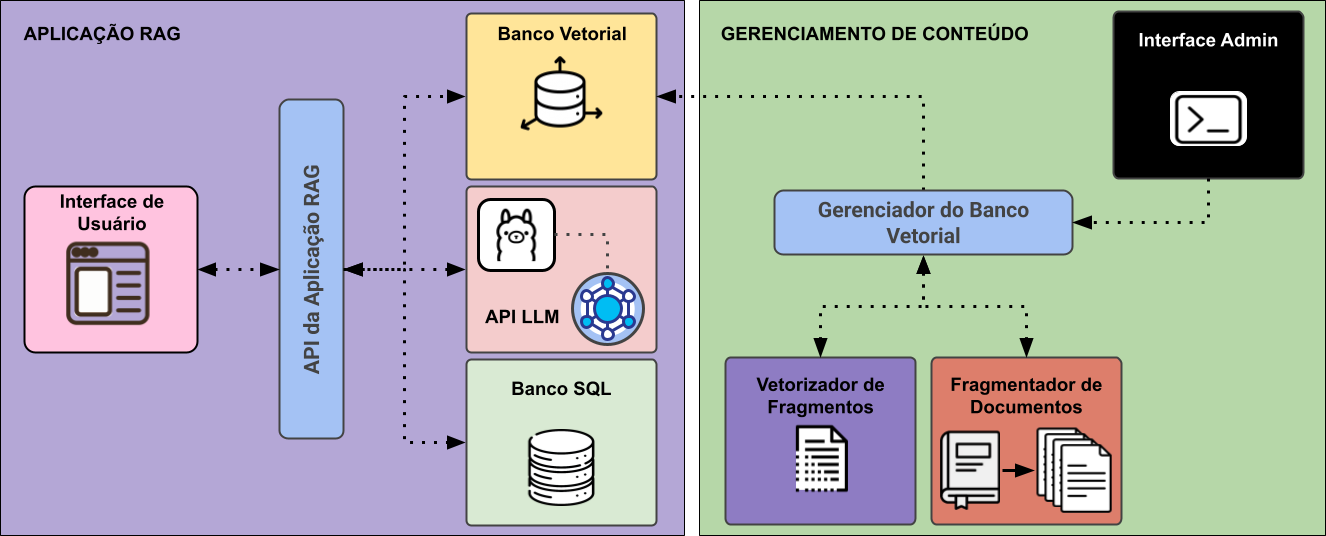
\includegraphics[width=1\linewidth]{Imagens/arquitetura.png}
    \caption{Arquitetura do Assistente de Buscas} 
    \label{fig:arq-assist-busca}
\end{figure}

% AFAZER: Alterar figura

\section{Banco Vetorial}
\label{sec:Assistente.1}
\subsection{Chroma DB}
\label{subsec:Assistente.1.1}

Conforme descrito pelos seus desenvolvedores e mantenedores \cite{Chroma:1}, o Chroma DB é um projeto concebido e mantido por uma equipe dedicada de especialistas da empresa Chroma, se tratando de um banco de dados vetorial de código aberto, cujo desenvolvimento tem foco na garantia de integração nativa com aplicações de inteligência artificial. A arquitetura do Chroma DB foi projetada para simplificar e agilizar o desenvolvimento de aplicações baseadas em \ac{LLM}s, fornecendo mecanismos que permitem a modularização de conjuntos de dados, informações e documentos, facilitando sua integração com \ac{LLM}s. O Chroma DB disponibiliza ferramentas robustas para o armazenamento e gerenciamento de documentos e seus metadados, assim como a criação e persistência de sua representação por \textit{embeddings}, possibilitando a realização de buscas de similaridade semântica sobre os dados de forma otimizada.

Entre os pontos fortes do Chroma DB estão a facilidade de implantação e utilização, assim como a priorização da produtividade dos desenvolvedores, sem comprometer a eficiência e a rapidez das operações por ele realizadas. O banco vetorial funciona como um serviço de servidor e vem acompanhado de SDKs de alta qualidade, escritos em Python e JavaScript/TypeScript, os quais fornecem todo o ferramental necessário a uma integração fluida em diversos tipos de projetos. Ademais, apresenta compatibilidade com ambientes de desenvolvimento interativos, como os populares notebooks Jupyter e IPython, promovendo uma experiência mais colaborativa e ágil para desenvolvedores e cientistas de dados.

O núcleo organizacional do Chroma DB são as coleções (\textit{collections}), sendo estruturas nas quais \textit{embeddings}, documentos e metadados relacionados são armazenados e por meio das quais são gerenciados. Sua utilização se dá de forma simples e direta, sendo necessário apenas lhe atribuir um nome e iniciar a inserção dos documentos, visto que o banco vetorial já se encarrega automaticamente da geração dos \textit{embeddings} e da indexação correspondente. Embora, por padrão, o banco já tenha definidas uma função de geração de \textit{embeddings} e uma métrica de similaridade padrão (o modelo \textit{all-MiniLM-L6-v2}, do \textit{Sentence Transformers}, e distância euclidiana, respectivamente), para cenários que exigem maior flexibilidade, a plataforma permite o fornecimento de uma função de geração de \textit{embeddings} personalizada, possibilitando a utilização de modelos específicos, que atendam às particularidades e características de comportamento desejadas. Analogamente, é possível configurar a medida de similaridade, de forma que ela utilize outras métricas, em vez da padrão, como, por exemplo, a distância do cosseno, reconhecidamente eficaz para medida de distância de vetores de \textit{embeddings}.

Uma vez processado, o documento, juntamente com seu  id, \textit{embeddings} e metadados são armazenados na coleção, sendo sua representação vetorial indexada para dar suporte à busca por similaridade de forma eficiente. O Chroma DB faz uso de estruturas otimizadas, como grafos do tipo HNSW (\textit{Hierarchical Navigable Small World}) ou algoritmos de \textit{approximate nearest neighbor} (ANN) para recuperação de documentos com \textit{embeddings} mais semelhantes de forma mais rápida e com bom desempenho.

As consultas em uma coleção são realizadas por meio de se informar listas de textos de entrada, a partir dos quais o banco de vetores retorna uma quantidade definida e ajustável de resultados semanticamente mais semelhantes aos termos informados. Os resultados da consulta incluem, além do conteúdo e metadados dos documentos retornados, o valor  da distância semântica entre cada um deles e o texto de entrada, permitindo uma análise com maior granularidade e a validação da relevância dos conteúdos. Essa capacidade de análise de similaridade de forma intuitiva permite posterior processamento intermediário dos resultados (como, por exemplo, a possibilidade de filtragem dos resultados e o estabelecimento de um limiar de exclusão de resultados com base em uma similaridade mínima desejada), oferecendo mais flexibilidade para o processo como um todo.

Quando da realização de uma consulta ao banco vetorial, em uma coleção específica, a mesma função de geração de \textit{embeddings} utilizada para gerar as representações vetoriais armazenadas é executada sobre o texto/documento fornecido como critério de busca, resultando, similarmente, em uma representação em formato de vetor de alta dimensionalidade. O Chroma DB, então, realiza a busca dentre os documentos vetorizados já armazenados por instâncias semanticamente mais semelhantes, utilizando a métrica de similaridade definida na criação da coleção, recuperando os documentos resultantes da busca.

\subsection{Modelo da função de \textit{embeddings}}
\label{subsec:Assistente.1.2}

Considerando a possibilidade oferecida pelo banco vetorial de se fornecer uma função de geração de \textit{embeddings} personalizada, sopesamos a utilização de diferentes modelos, levando em conta seu desempenho para fins de cálculo de similaridade -- levando em conta, especificamente, os resultados sobre a amostra de dados utilizada neste estudo. Dentre os modelos avaliados, a opção feita foi pelo INSTRUCTOR-XL. Trata-se de um modelo desenvolvido pela equipe de pesquisa de Processamento de Linguagem Natural (NLP) da Universidade de Hong Kong, incluindo a participação de pesquisadores de outras instituições, como \textit{University of Washington}, Meta AI e \textit{Allen Institute for AI}, publicado em 2023 \cite{Instructor:1}. O modelo selecionado pertence à série de modelos INSTRUCTOR, que são projetados para gerar \textit{embeddings} de texto de alta qualidade e se baseiam na arquitetura Transformer, assim como modelos de estado da arte, como \ac{BERT} e \c{GPT}.

No trabalho de  \citeonline{Instructor:2}, os seus publicadores o definem como \textit{“One Embedder [for] Any Task”} e como

\begin{citacao}
    an instruction-finetuned text embedding model that can generate text embeddings tailored to any task (e.g., classification, retrieval, clustering, text evaluation, etc.) and domains (e.g., science, finance, etc.) by simply providing the task instruction, without any finetuning. \footnote{Um modelo de geração de \textit{embeddings} textuais com \textit{fine-tuning} feito a partir de uma instrução, capaz de gerar \textit{embeddings} de texto otimizados para qualquer tarefa (tais como, classificação, recuperação, agrupamento, avaliação de texto, etc.) e quaisquer domínios (quais sejam ciência, finanças, etc.) simplesmente fornecendo a instrução da tarefa, sem necessidade de \textit{fine-tuning} tradicional. (Tradução nossa)}
\end{citacao}

Os INSTRUCTORs são, portanto, modelos de criação de \textit{embeddings} textuais de forma adaptativa, a partir da inclusão de instruções em linguagem natural, as quais atuam como direcionadores de ajuste fino, demonstrando bom desempenho em não somente “compreender” texto em um sentido mais aberto e genérico, sendo capaz de interpretá-lo com uma visão direcionada a aplicações e casos de uso particulares. Desta forma, as representações vetoriais geradas são otimizadas para tarefas específicas (como classificação, recuperação de informações, agrupamento, avaliação semântica, entre outras) e/ou domínios diferentes sem a necessidade de refinamento do modelo nos moldes tradicionais de \textit{finetuning}, tornando-o adaptável e mais relevante para diversas aplicações.
A versão utilizada no Assistente de Busca, especificamente, é a \textit{instructor-xl}, sendo a variante dentre a família de modelos INSTRUCTOR com maior tamanho, otimizada para desempenho e equilíbrio entre precisão e eficiência em aplicações de processamento de linguagem natural.

\section{Geração de Conteúdo}
\label{sec:Assistente.2}

\subsection{LLaMA}
\label{subsec:Assistente.2.1}
O modelo LLaMA (\textit{Large Language Model Meta AI}) ou simplesmente Llama, foi proposto em artigo de fevereiro de 2023 \cite{Llama:1}, havendo sido projetado para pesquisas avançadas em \ac{PLN}. Sua publicação se deu com a intenção da Meta AI, responsável pelo desenvolvimento do modelo, de disponibilizar acesso por parte da comunidade acadêmica e de desenvolvedores a um recurso de alta capacidade, permitindo-lhes explorar aplicações de \ac{IA} e experimentar inovações em grandes modelos de linguagem.

Baseado na arquitetura \textit{Transformers}, similar ao modelo \ac{GPT}, o Llama é otimizado para balancear desempenho e eficiência, estando apto a ser utilizado em tarefas como geração de texto, resumo de documentos, tradução automática, e resposta a perguntas. Tendo várias versões com tamanhos que variam de 7 bilhões (7B) a 65 bilhões (65B) de parâmetros, a  coleção de modelos permite a escolha de uma opção mais adequada, conforme a aplicação desejada e os recursos computacionais disponíveis.

A Meta AI, em sua introdução ao projeto, afirma que o Llama foi projetado como alternativa a outros \ac{LLM}s, como o GPT da OpenAI, com foco em ser mais eficiente em termos de recursos computacionais. Nesse contexto, o modelo é definido como
\begin{citacao}
    a state-of-the-art foundational large language model designed to help researchers advance their work in this subfield of AI. Smaller, more performant models such as LLaMA enable others in the research community who don’t have access to large amounts of infrastructure to study these models, further democratizing access in this important, fast-changing field. \cite{Llama:2} \footnote{um LLM de propósito geral, de última geração, projetado para ajudar pesquisadores a avançarem em seus trabalhos neste subcampo da IA. Modelos menores e mais eficientes, como o LLaMA, permitem que outros na comunidade de pesquisa que não têm acesso a grandes infraestruturas estudem esses modelos, democratizando ainda mais o acesso a este campo importante e em rápida evolução. (Tradução nossa)}
\end{citacao}


Um dos pontos fortes do Llama no contexto dos \ac{LLM}s é precisamente este fato de ele exigir um poder computacional consideravelmente reduzido e recursos mais modestos em comparação com outros modelos de referência à época de seu lançamento, sendo, pela natureza de seu treinamento -- baseado em dados não rotulados -- ideal para ser refinado para uma ampla gama de aplicações e tarefas.

O artigo de publicação do modelo aponta que o treinamento do Llama incluiu um número de \textit{tokens} na ordem de trilhões e utilizou exclusivamente conjuntos de dados publicamente disponíveis, sem contar com dados em bancos de dados proprietários ou de acesso restrito. Quando do lançamento da versão original, a versão do Llama com 13 bilhões de parâmetros ofereceu melhor desempenho que o GPT-3, que utiliza 175 bilhões de parâmetros; assim como o LLaMA65B se mostrou  competitivo com modelos maiores, como Chinchilla-70B e PaLM-540B (com 70 e 540 milhões de parâmetros, respectivamente).

Ao realizar o lançamento do Llama, em fevereiro de 2023, com o intuito de manter a integridade e evitar o potencial mau uso do modelo mediante uma publicação não supervisionada, a Meta AI optou por realizar a disponibilização sob uma licença de uso não-comercial, com foco em aplicações para fins de pesquisa, apenas. O acesso ao modelo, então, era garantido mediante análise caso a caso para acadêmicos, para organizações civis e governamentais, como também para laboratórios da indústria internacional, a qual se seguia à submissão de manifestação de interesse.

No início do semestre seguinte, a Meta disponibilizou mais uma versão do modelo, o Llama 2 \cite{Llama:3}. Nessa nova liberação, foi tornado disponível, sem custos para pesquisas e uso comercial, os pesos e o código de inicialização para a versão pré-treinada e direcionada à conversação. Aprimoramentos foram aplicados por meio do uso de técnicas que consideram \textit{feedback} humano, como \textit{Reinforcement Learning with Human Feedback} (RLHF), coleta de dados sobre preferência nas interações com humanos,  modelagem de recompensa e uma técnica simples para evitar degradação na qualidade no seguimento das instruções dadas ao modelo, chamada \textit{Ghost Attention} (GAtt). \cite{Llama:4}

No ano de 2024, em maio, julho e novembro, a Meta AI fez o lançamento de atualizações do Llama, com suas versões 3, 3.1 e 3.2, respectivamente. Cada uma das versões trouxe avanços significativos em relação às diversas iterações do Llama 2, em especial no número de parâmetros (405 bilhões). O \textit{paper} de lançamento do Llama 3 o descreve como:
\begin{citacao}
    a herd of language models that natively support multilinguality, coding, reasoning, and tool usage, [whose largest version] is a dense Transformer with 405B parameters and a context window of up to 128K tokens [delivering] comparable quality to leading language models such as GPT-4 on a plethora of tasks. \cite{Llama:5} \footnote{um conjunto de modelos de linguagem com suporte nativo a multi-idiomas, codificação, raciocínio e uso de ferramentas, [cuja maior versão] é um Transformer denso com 405 bilhões de parâmetros e uma janela de contexto de até 128 mil tokens, [oferecendo] qualidade comparável a modelos de linguagem de ponta, como o GPT-4, em uma ampla variedade de tarefas. (Tradução nossa)}
\end{citacao}


A versão mais recente até a escrita deste estudo, o Llama 3.2, se intitula como um conjunto de modelos customizáveis com inteligência artificial de ponta e revolucionária, dados os avanços que demonstrou. Além de manter uma versão anterior, Llama 3.1, com o tamanho pleno de 405 bilhões de parâmetros, foram disponibilizadas, com o Llama 3.2, versões mais leves, com 1 e 3 bilhões de parâmetros, as quais apresentam capacidade de geração de texto em múltiplos idiomas, otimizadas para serem leves e realizarem sumarização e reescrita de texto, execução de instruções e tarefas afins localmente, \textit{on-device}. As versões médias, com 11 e 90 bilhões de parâmetros, além das capacidades textuais, suportam usos de caso de compreensão de imagem. Dentre as possibilidades, são citadas

\begin{citacao}
    document-level understanding including charts and graphs, captioning of images, and visual grounding tasks such as directionally pinpointing objects in images based on natural language descriptions. \cite{Llama:6} \footnote{compreensão em nível de documento, incluindo gráficos e tabelas, descrição de imagens e tarefas de correspondência visual, como identificação direcional de objetos em imagens com base em descrições em linguagem natural. (Tradução nossa)}
\end{citacao}

Conforme declarado pela própria Meta AI, o foco do Llama 3.2 se dá sobre a disponibilização de versões mais leves, ao custo de uma quantidade menor de parâmetros (3 milhões, na versão dita padrão, em vez de 405 da versão 3.1). Apesar do tamanho reduzido, o desempenho é ainda muito promissor para diversas tarefas de processamento de linguagem natural.

\subsection{Ollama}
\label{subsec:Assistente.2.2}
O Ollama foi utilizado como ferramenta facilitadora, de forma a fazer uso do Llama3.1 como a etapa final do processo de recuperação da informação com base no texto informado pelo usuário. Trata-se de um \textit{framework} de código aberto e multiplataforma cujo desenvolvimento foi realizado por uma equipe da empresa Ollama Inc., baseado no llama.cpp -- uma biblioteca de alto desempenho escrita em C++ e otimizada para utilização de \ac{LLM}s.

Tal ferramenta foi projetada com fins específicos de simplificar a implementação e operação de \ac{LLM}s sem a necessidade de infraestrutura em nuvem; o que permitiu o acesso e gerenciamento de modelos diversos, tais qual o Llama 3.1 e outras arquiteturas avançadas em máquinas locais. Essa abordagem promove maior privacidade, ao evitar a necessidade de envio dedados a servidores de terceiros, além de reduzir os custos operacionais, eliminando as taxas associadas à inferência baseada em nuvem. \cite{Ollama:1}

A plataforma oferece suporte tanto para hardware de uso comum quanto para equipamentos de alto desempenho, provendo otimização do uso de GPUs durante a utilização de modelos de diferentes níveis de complexidade, incluindo aqueles com bilhões de parâmetros. A interação com o \ac{LLM} em si é mediada pelo Ollama, o qual fornece tanto uma interface de linha de comando -- a qual é executada na máquina em que a ferramenta está instalada -- quanto uma forma de interação programática, por meio de uma API REST, permitindo integração com aplicações de diversos tipos e usos.

Além disso, o Ollama dispõe de uma variedade de modelos que podem ser instalados de forma ágil e simplificada, permitindo acessá-los e utilizá-los de forma rápida e sem empecilhos, tanto para lhes fazer uso tal qual são disponibilizados, quanto para lhes aplicar ajustes específicos, buscando atender a domínios particulares.


\chapter{Metodologia}
\label{cap:Metodologia}

Dado que no Capítulo \ref{cap:Assistente} tratamos de apontar \textit{o que será desenvolvido}, neste capítulo buscamos expor \textit{os meios que usaremos} para alcançar o que nos propomos. Abordaremos, portanto, a definição de todos os elementos componentes da solução proposta, bem como os critérios utilizados nas tomadas de decisão quanto a recortes de dados de entrada e seu tratamento e preparação, modelos utilizados, critérios de avaliação e afins. Começamos, na Seção \ref{sec:Metodologia.1}, apontando a forma de preparação dos dados a serem consultados e usados como base para a geração final das respostas (sua seleção, tratamento, preparação e persistência no banco vetorial). A Seção \ref{sec:Metodologia.2} trata das decisões tomadas para realizar a melhor  configuração para o banco vetorial. As Seções \ref{sec:Metodologia.3} e \ref{sec:Metodologia.4} abordam, respectivamente, (1) a configuração do ambiente de execução do \ac{LLM} e (2) sua integração com os dados recuperados do banco vetorial -- efetivamente definindo a estrutura \ac{RAG}. A exposição da aplicação ao usuário, por meio de uma interface web simples é descrita na Seção \ref{sec:Metodologia.5}, ao passo que as medições dos resultados e avaliações são apresentadas na Seção \ref{sec:Metodologia.6}.

\section{Definição do Conjunto de Dados}
\label{sec:Metodologia.1}

Estabelecida a abordagem a ser utilizada para o desenvolvimento da ferramenta proposta, tornou-se necessário definir quais conjuntos de dados/documentos seriam incluídos no processo de desenho, implementação, testes e validação dos resultados. Dado que, conforme apresentado na Seção \ref{sec:DocAlern.1}, há, no contexto da \ac{Alern}, diferentes conjuntos de documentos com características diversas, tanto mais estáticos quanto extremamente dinâmicos, era necessário começar definindo que tipos de documentos e quais domínios dentre todos seriam significativos.

A escolha dos dados para desenvolvimento foi feita com o intuito de se alcançar dois objetivos específicos. O primeiro seria garantir que o objeto final dessa fase preliminar de desenvolvimento pudesse ser de uso relevante para a Casa Legislativa, tanto em termos de funcionalidade, mas também no sentido de abarcar um conjunto de informações que seja de interesse e relevância aos usuários do público interno ou externo à \ac{Alern}. Além deste, pretende-se assegurar que o domínio em que se enquadre o corpus escolhido coincida com as áreas de conhecimento e atuação dos integrantes do grupo de especialistas que se voluntariaram a avaliar a qualidade das respostas geradas. Com isso, seria potencializado o processo de testes e validação dos resultados da aplicação, tanto pelo volume de pessoas que poderão utilizar na fase de testes -- dado que informações escolhidas de forma estratégica atrairão mais usuários -- quanto pela qualidade do conhecimento dos avaliadores.

O recorte de documentos selecionados para compor o corpus textual sobre o qual esta proposta atuará foi feito sob sugestão e orientação de servidores atuantes nos setores de gestão de pessoas (CDHO - Coordenadoria de Desenvolvimento Humano e Organizacional) e setores envolvidos em diversas fases do processo legislativo -- em especial por serem a gestão de pessoas e o processo legislativo duas áreas da \ac{Alern} em que é comum o surgimento de dúvidas procedimentais, bem como a busca por informações que pautem ou desabonem uma ou outra medida a ser tomada ou ações dos servidores em geral. A coleção de documentos inclui a normatização e regimentação da atuação parlamentar, a regulação de direitos e deveres dos servidores (em especial no que se refere a benefícios/auxílios, cálculo de vencimentos, férias e bonificações), planos de cargos e carreiras, avaliação do servidor em estágio probatório de trabalho, assim como o regime jurídico dos servidores do Rio Grande do Norte (dos quais os servidores da \ac{Alern} são um subconjunto).

Os documentos selecionados têm suas características detalhadas nas Tabelas \ref{tab:descricao-documentos-1} e \ref{tab:descricao-documentos-2}. A Tabela \ref{tab:descricao-documentos-1} contém os quantitativos de \textit{tokens}, palavras e artigos em cada documento. A Tabela \ref{tab:descricao-documentos-2}, por sua vez, caracteriza a distribuição média de palavras e \textit{tokens} por artigo, em cada documento, bem como expõe a quantidade de artigos com mais de 300 palavras e com mais de 500 \textit{tokens} em cada documento -- sendo esse segundo dado algo relevante de se considerar, dado a limitação da quantidade de \textit{tokens} suportada por modelos específicos (ver início da Seção \ref{subsec:Metodologia.1.1} para mais detalhes).

Os documentos descritos nas Tabelas \ref{tab:descricao-documentos-1} e \ref{tab:descricao-documentos-2} -- identificados na primeira coluna de cada uma -- são
os seguintes:

\begin{enumerate}
    \item Lei Complementar Estadual Nº 122/1994
    \item Resolução Nº 031/2021 – Alern
    \item Resolução Nº 075/2024 – Alern
    \item Resolução Nº 078/2024 – Alern
    \item Resolução Nº 106/2018 – Alern
    \item Resolução Nº 2388/2019 – Alern
    \item Resolução Nº 077/2024 – Alern
    \item Resolução Nº 089/2017 – Alern
    \item Resolução Nº 618/2022 – Alern
    \item Resolução Nº 064/2022 – Alern
    \item Resolução Nº 133/2025 – Alern
    \item Manual de Processo Legislativo - Alern
\end{enumerate}

\begin{table}
    \caption{Quantitativos de Palavras/\textit{Tokens}/Artigos por Documento}
    \centering
    \begin{tabular}{ c c c c }
        \hline
        \textbf{Documento} & \textbf{palavras} & \textbf{\textit{tokens}} & \textbf{artigos} \\  
        \hline
        1 & 15.228 & 23.079 & 245 \\
        2 & 43.579 & 65.850 & 376 \\
        3 & 651 & 1.197 & 7 \\
        4 & 1.778 & 2.648 & 21 \\
        5 & 4.735 & 6.903 & 46 \\
        6 & 1.573 & 2.329 & 14 \\
        7 & 511 & 758 & 7 \\
        8 & 4.361 & 6.306 & 41 \\
        9 & 1.024 & 1.546 & 9 \\
        10 & 432 & 651 & 7 \\
        11 & 1.891 & 2.881 & 25 \\
        12 & 19.710 & 30.036 & ** \\
        \hline
    \end{tabular}
    
    \small \textbf{**Nota}: texto não articulado.
    
    Fonte: O autor (2025)
    \label{tab:descricao-documentos-1}
\end{table}

\begin{table}
    \caption{Quantitativos Palavras e \textit{Tokens} por Artigo em cada Documento}
    {
        \centering
        \begin{tabular}{ c c c c c }
            \hline
            \textbf{Documento} & \textbf{pals./art.} & \textbf{tokens/art.} & \textbf{arts. 300+ pals} & \textbf{arts. 500+ tokens} \\  
            \hline
            1 & 62,2 & 94,2 & 2 & 7 \\
            2 & 115,9 & 175,1 & 33 & 58 \\
            3 & 93,0 & 171,0 & 1 & 1 \\
            4 & 84,7 & 126,1 & 1 & 1 \\
            5 & 102,9 & 150,1 & 2 & 6 \\
            6 & 112,4 & 166,4 & 1 & 3 \\
            7 & 73,0 & 108,3 & 0 & 0 \\
            8 & 106,4 & 153,8 & 2 & 6 \\
            9 & 113,8 & 171,8 & 1 & 3 \\
            10 & 61,7 & 93,0 & 0 & 0 \\
            11 & 75,64 & 114,76 & 0 & 0 \\
            12 & ** & ** & ** & ** \\
            \hline
        \end{tabular}
    }

    \small \textbf{**Nota}: texto não articulado.\\
    \small \textbf{pals./art.}: Média do número de palavras por artigo \\
    \small \textbf{tokens/art.}: Média do número de \textit{tokens} por artigo \\
    \small \textbf{arts. 300+ pals}: Número de artigos com mais de 300 palavras \\
    \small \textbf{arts. 500+ tokens}: Número de artigos com mais de 500 \textit{tokens} \\
    
    {\centering
        Fonte: O autor (2025)\par
    }
    \label{tab:descricao-documentos-2}
\end{table}

Ao se analisar os elementos do conjunto de documentos selecionados, é possível perceber que há certo grau de homogeneidade entre os documentos em alguns quesitos. Alguns exemplos de proximidade entre esses componentes são a interrelação entre as temáticas, as suas estruturas semelhantes entre si, seguindo a divisão padrão de textos normativos -- com capítulos, seções, artigos, parágrafos, alíneas, etc. --, o tom do vocabulário e o estilo da escrita característicos de texto legislativo, entre outros. Essa homogeneidade, em especial no que se refere à estrutura, facilita sua manipulação, sua eventual fragmentação e seu processamento, em preparação para sua inclusão no fluxo de atividades do sistema.

Não obstante, também é facilmente perceptível que os exemplares da lista de documentos possuem características distintas entre si: há variação considerável no comprimento dos documentos como um todo, alguns são apenas leis que alteram a redação de outra peça existente no conjunto sem oferecer outros conteúdos, entre outras características que os diferenciam entre si. Também é relevante essa disparidade, visto que, mesmo dentro de um contexto de documentos semi-estruturados, há diversidade suficiente para que seu tratamento seja adequado e aplicável a textos puramente não estruturados.

Uma característica peculiar do conjunto de dados utilizado é a possibilidade de documentos normativos diferentes estabelecerem como fatos informações conflitantes e se contradizerem. Há duas situações, que conseguimos prever, nas quais é possível que haja choque de informações: atualização da regulação e especificidades hierárquicas.

A primeira se dá pelo motivo de que, pela própria dinâmica da atividade legislativa, determinadas leis/normas são atualizadas, modificadas ou criadas com o tempo; de forma que algo que é estabelecido como fato hoje pode ser impactado por um novo ato normativo, por alteração do texto da lei, por sua revogação e afins. De forma a mitigar essa problemática, é necessária a manutenção dos documentos e suas representações vetoriais, garantindo que sua versão mais atualizada (preferencialmente a versão compilada de seu texto) seja a disponibilizada pelo banco vetorial.

A segunda se dá quando uma peça normativa de abrangência maior prevê algo, enquanto um ato normativo de alcance específico preveem, paradoxalmente, coisas distintas. Um caso específico, para fins de demonstração, é o fato de o Regime Jurídico dos servidores públicos civis do Estado do Rio Grande do Norte determina que:

\begin{citacao}
    A gratificação natalina, devida a ocupante de cargo efetivo ou em comissão, corresponde a 1/12 (um doze avos) da remuneração a que fizer jus no mês de dezembro, por mês de exercício no respectivo ano \cite{RegimeJuridico:RN}.
\end{citacao}


Assim, enquanto no âmbito mais amplo do Estado do RN a gratificação natalina é calculada unicamente em função da remuneração base do servidor, a Resolução Nº 77, de 10 de julho de 2024 \cite{RegimentoInterno:ALRN}, que trata da base de cálculo do terço de férias e da gratificação natalina (13º salário) especificamente dos servidores da \ac{Alern} prevê que:
\begin{citacao}
    Fica determinado que os valores percebidos a título de auxílio-alimentação e auxílio de assistência à saúde, por se tratarem de vantagens pecuniárias que compõem a remuneração do servidor, serão incluídos na base de cálculo do terço constitucional de férias e da gratificação natalina (13º salário) dos servidores e, naquilo que couber, dos membros da Assembleia Legislativa do Estado do Rio Grande do Norte.
\end{citacao}

Como ambos os documentos estão disponíveis no banco vetorial, uma busca por ``Os valores recebidos como auxílio-alimentação compõem a base de cálculo para a gratificação natalina?'' pode resultar no retorno de ambos os fragmentos, provendo ao \ac{LLM} informações conflitantes, visto que não foi fornecido um contexto na pergunta. Embora seja possível uma abordagem mais efetiva para a resolução deste problema (como uma organização hierárquica -- em termos de abrangência -- dos documentos), no escopo deste estudo, limitamo-nos a informar ao \ac{LLM}, junto com o texto do fragmento, o seu título e autor, que por si só já delimitam o âmbito em que a peça normativa se aplica.

\subsection{Tratamento dos Dados Selecionados}
\label{subsec:Metodologia.1.1}

Feita a coleta dos arquivos com os textos dos documentos elencados para a composição do conjunto a ser utilizado, foi necessário definir como o texto seria tratado. Os aspectos de particionamento dos documentos e da manutenção do contexto do conteúdo são abordados nas Seções \ref{subsubsec:Metodologia.1.1.1} e \ref{subsubsec:Metodologia.1.1.2}, respectivamente.

\subsubsection{Fragmentação do Conteúdo}
\label{subsubsec:Metodologia.1.1.1}

Um dos aspectos que deve ser levado em consideração é a garantia de que o tamanho de seu conteúdo seja adequado às limitações das ferramentas de geração de representação vetorial do texto. Ignorar essas características de cada modelo pode levar à perda de informação quando da geração dos \textit{embeddings} dos documentos, dado que os modelos truncam parte do conteúdo sobre o qual operarão, nos casos em que o número máximo de \textit{tokens} que conseguem processar é extrapolado. A divisão ou particionamento do conteúdo textual dos documentos é a parte central desse processo.

Considerando que diversos modelos selecionados para avaliação na inclusão das funções de geração de \textit{embeddings} neste trabalho (ver Tabela \ref{tab:num-maximo-tokens} na Seção \ref{subsubsec:Metodologia.2.1.6}) têm uma limitação no número de \textit{tokens} de entrada para geração da representação em vetores (em geral 512 \textit{tokens}), visto que se baseiam na arquitetura \textit{Transformer}, \cite{Instructor:3}, a escolha feita foi pela fragmentação de cada um dos documentos em porções de texto com um número máximo de 300 palavras. Com isso, cada fragmento de um documento seria tratado pelo Chroma DB como um documento por si só, ficando sua relação de pertencimento registrada nos metadados, para casos de eventuais  buscas pelo documento como um todo. Dessa forma, ao serem \textit{tokenizados} os fragmentos dos documentos no conjunto, as representações vetoriais resultantes ficam dimensionadas de forma a respeitar a limitação de tamanho da entrada recebida pelo modelo utilizado, eliminando a necessidade de supressão de informações por truncamento dos \textit{tokens} excedentes.

A fragmentação do volume do texto de fato é desejável e otimiza o processo de recuperação de documentos (fragmentos menores permitem maior granularidade no cálculo da semelhança semântica com o \textit{input} do usuário), além de reduzir o tamanho geral do \textit{prompt} a ser fornecido ao \ac{LLM} para geração do conteúdo sintético a responder a pergunta feita, visto que este incluirá o conteúdo dos fragmentos recuperados. Todavia, a divisão do conteúdo considerando meramente o tamanho de cada fragmento pode implicar em dispersão de contexto, colocando uma parte de uma ideia em um fragmento, isolando-a de sua parte complementar alocada em outro, de forma que a ideia completa se perde no instante da recuperação de documentos, podendo não ser identificada pela busca semântica de similaridade.

\subsubsection{Manutenção do Contexto}
\label{subsubsec:Metodologia.1.1.2}

Considerando o exposto na Seção anterior, é igualmente crucial mitigar a fragmentação e dispersão do contexto dos dados, evitando que informações correlacionadas -- e contíguas, no texto original -- se encontrem espalhadas ao longo de diversos fragmentos ao final do processo de divisão dos documentos em pedaços menores. Para isso é importante compreender que o sentido, o significado e a semântica comunicados residem não somente o conteúdo textual, nas palavras expressas do texto, senão também no que se infere a partir do que os precedeu, seja a nível textual ou estrutural.

Assim, realizar a divisão do documento garantindo que os pontos de quebra aconteçam entre uma frase e outra -- depois de um ponto final/interrogação/exclamação -- garante que ideias não sejam quebradas no nível da frase, reduzindo em parte a fratura de contexto que se realiza considerando meramente o número de palavras/\textit{tokens} do fragmento final. Igualmente, a garantia de que a quebra acontece em um ponto que divide duas unidades com um grau maior de completude de uma ideia avança na direção de se obter fragmentos semanticamente autocontidos, com menor dependência de conteúdo conseguinte ou, ainda mais, precedente. Com efeito, o contexto precedente possui impacto maior sobre a completude de uma partição do documento do que aquele que a sucede.

Além da informação textual que antecede certo excerto, muito sentido é codificado na estrutura do documento em si -- em especial nos casos de documentos formalmente estruturados e/ou organizados de forma hierárquica. 

Considere, por exemplo, o texto seguinte organizado hierarquicamente:

\fbox{%
  \parbox{0.75\linewidth}{%
    \raggedright \sffamily
    \textbf{Preparação do Ambiente} \\
    Como forma de facilitar o processo de adaptação, mudanças e atualização, optamos por adotar um cliente LLM chamado Ollama. Mais informações a respeito em \href{https://ollama.com/}{https://ollama.com/}.

    \vspace{6pt}
    \textbf{Linux} \\

    \textbf{Como instalar o Ollama}
    \begin{itemize}
      \item No terminal, baixe e execute o script de instalação:
      \item \texttt{curl -fsSL https://ollama.com/install.sh | sh}
    \end{itemize}

    \textbf{Como definir as variáveis de ambiente}
    \begin{itemize}
      \item \texttt{export OLLAMA\_MAX\_LOADED\_MODELS=5}
      \item \texttt{export OLLAMA\_DEBUG='true'}
    \end{itemize}

    \vspace{6pt}
    \textbf{Windows} \\

    \textbf{Como instalar o Ollama}
    \begin{itemize}
      \item Acesse a página de download do Ollama no link \href{https://ollama.com/download/windows}{https://ollama.com/download/windows} e faça o download do instalador.
      \item Execute o instalador e siga as instruções em tela.
    \end{itemize}

    \textbf{Como definir as variáveis de ambiente}

    \textbf{Powershell}
    \begin{itemize}
      \item \texttt{\$env:OLLAMA\_MAX\_LOADED\_MODELS=5; \$env:OLLAMA\_DEBUG=`true'}
    \end{itemize}

    \textbf{Prompt}
    \begin{itemize}
      \item \texttt{set OLLAMA\_MAX\_LOADED\_MODELS=5}
      \item \texttt{set OLLAMA\_DEBUG=`true'}
    \end{itemize}
  }
}

Ignorando o comprimento diminuto de cada uma das seções -- tomando-as como mais longas -- vemos que temos duas seções com informações diferentes de como instalar o Ollama. O que as torna coerentes não é o conteúdo de cada uma, mas o ponto da hierarquia da estrutura textual em que ambas se localizam. Destarte, é necessário ``injetar'' no texto dos fragmentos que compõem ambas essas seções informações sobre sua posição na estrutura hierárquica do documento.

O mesmo princípio se aplica a documentos articulados, como peças legislativas, em que as alíneas e parágrafos, por exemplo, só têm coerência semântica quando vinculados com as informações antecedentes, dentro do mesmo artigo.

\subsubsection{Documentos Articulados}
\label{subsubsec:Metodologia.1.1.3}

Diante do exposto, como uma abordagem para minimizar essa dispersão contextual, o processo de segmentação dos documentos se utilizou da estrutura intrínseca de cada um deles (divisão em artigos, parágrafos, alíneas e afins, nos casos de documentos articulados), de forma que os fragmentos ficaram orientados à divisão por artigo, dado que cada artigo é uma unidade autocontida, semanticamente coerente, sendo, no grosso dos exemplos, independente dos outros artigos, salvo quando de citação e referência. Mais claramente, cada documento foi segmentado de tal sorte que cada artigo compõe um fragmento. Apesar disso, conforme se vê na Tabela \ref{tab:descricao-documentos-2}, ainda há, no corpus selecionado, 43 artigos cujo teor textual ultrapassa o número de 300 palavras (via de regra por conter um grande número de parágrafos, incisos e alíneas), incorrendo no mesmo problema que ora é abordado, exceto que em um número muito menor de ocorrências, dada a raridade de artigos longos no conjunto de dados em questão.

Como uma forma de evitar essa situação, a abordagem adotada foi, nos casos de artigos mais extensos, secionar adicionalmente o artigo, em suas partes menores (caput, parágrafos, incisos e alíneas) e agrupá-las de forma que cada um desses agrupamentos consista de uma combinação do caput e parágrafos/incisos/alíneas cujo comprimento total não ultrapasse o limite escolhido de 300 palavras, conforme a Figura \ref{fig:fragmentacao-artigos}. Assim, embora essa fragmentação automatizada -- independente de divisão feita sob análise caso a caso -- não resolva o problema em sua completude, ao se garantir que cada um desses segmentos mantenha o contexto geral do artigo, condensado no caput, mitiga-se uma fragmentação extrema da ideia geral do artigo, obtendo-se uma coesão maior do que haveria no caso da divisão com base somente no número de palavras.

\begin{figure}[H]
    \centering
    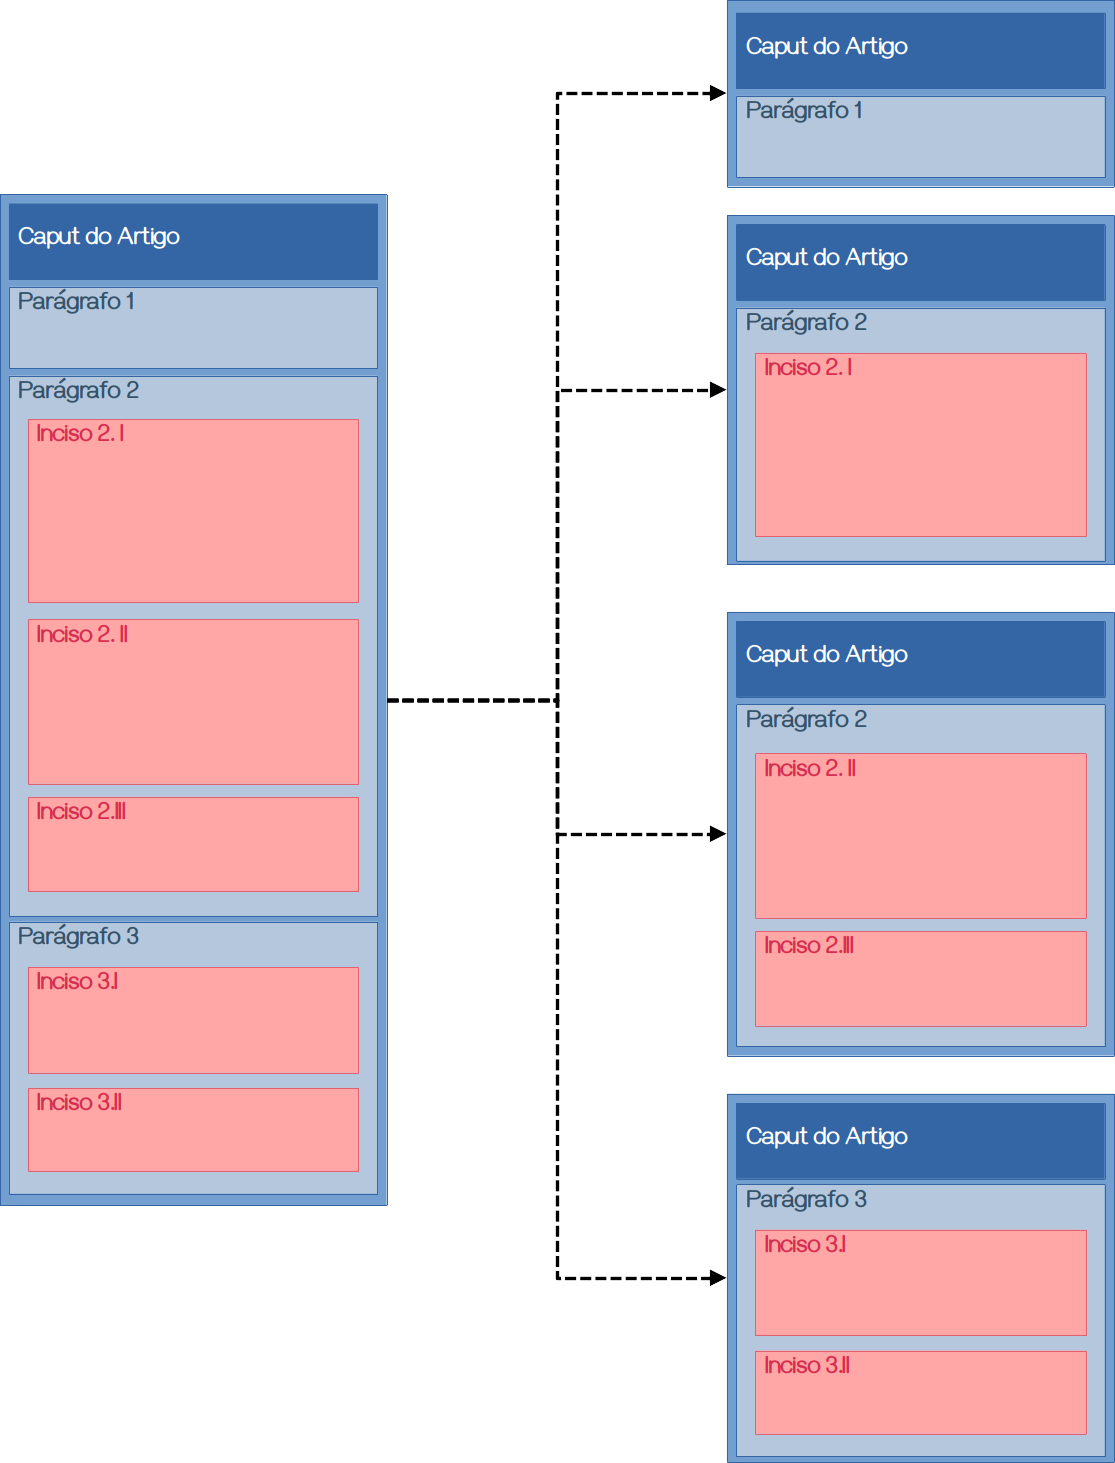
\includegraphics[width=0.5\linewidth]{Imagens/fragmentacao-artigos.png}
    \caption{Estratégia de Fragmentação de Artigos Extensos}
    Fonte: autoria própria
    \label{fig:fragmentacao-artigos}
\end{figure}

O resultado final do quantitativo de fragmentos por documento articulado está descrito na Tabela \ref{tab:descricao-fragmentos-1}.

\begin{table}[H]
    \caption{Quantitativos de artigos e Fragmentos por Documento}
    {
        \centering
        \begin{tabular}{ l c c c }
            \hline
            \textbf{Documento} & \textbf{Artigos} & \textbf{300+} & \textbf{Fragmentos} \\  
            \hline
            1. Lei Complementar Estadual Nº 122/1994 & 245 & 2 & 248 \\
            2. Resolução Nº 031/2021 – Alern & 376 & 33 & 420 \\
            3. Resolução Nº 075/2024 – Alern & 7 & 1 & 8 \\
            4. Resolução Nº 078/2024 – Alern & 21 & 1 & 22 \\
            5. Resolução Nº 106/2018 – Alern & 46 & 2 & 48 \\
            6. Resolução Nº 2388/2019 – Alern & 14 & 1 & 15 \\
            7. Resolução Nº 077/2024 – Alern & 7 & 0 & 7 \\
            8. Resolução Nº 089/2017 – Alern & 41 & 2 & 44 \\
            9. Resolução Nº 618/2022 – Alern & 9 & 1 & 10 \\
            10. Resolução Nº 064/2022 – Alern & 7 & 0 & 7 \\
            11. Resolução Nº 133/2025 - Alern & 25 & 0 & 25 \\
            12. Manual de Processo Legislativo & ** & ** & 244 \\
            \hline
        \end{tabular}
    }

    \small \textbf{**Nota}: O Manual de Processo Legislativo não é articulado (ver Seção \ref{subsubsec:Metodologia.1.1.4}) \\
    \small \textbf{300+}: Número de artigos com mais de 300 palavras \\
    
    {\centering
        Fonte: O autor (2025)\par
    }
    \label{tab:descricao-fragmentos-1}
\end{table}


\subsubsection{Documento Hierárquico}
\label{subsubsec:Metodologia.1.1.4}

Para realizar o particionamento do documento não articulado (O Manual de Processo mencionado e descrito na Seção \ref{sec:Metodologia.1}, mais especificamente nas Tabelas \ref{tab:descricao-documentos-1} e \ref{tab:descricao-documentos-2}), nos apoiamos em sua estrutura hierárquica. Definimos o limite de tamanho do fragmento tal qual no caso de documentos articulados (Seção \ref{subsubsec:Metodologia.1.1.1}) e aplicamos a ideia de autocontenção de conteúdo nos fragmentos, de forma que cada um deles tenha o máximo de autonomia semântica possível (Seção \ref{subsubsec:Metodologia.1.1.2}).

Dado que o documento não é articulado, tomamos como unidade semanticamente atômica o parágrafo. E como forma de injetar informação sobre o contexto hierárquico a que o fragmento pertence, lançamos mão dos cabeçalhos de cada seção/subseção no nível superior ao do fragmento. A Figura \ref{fig:fragmentacao-hierarquico} mostra a estratégia de particionamento de arquivos hierárquico.

\begin{figure}[H]
    \centering
    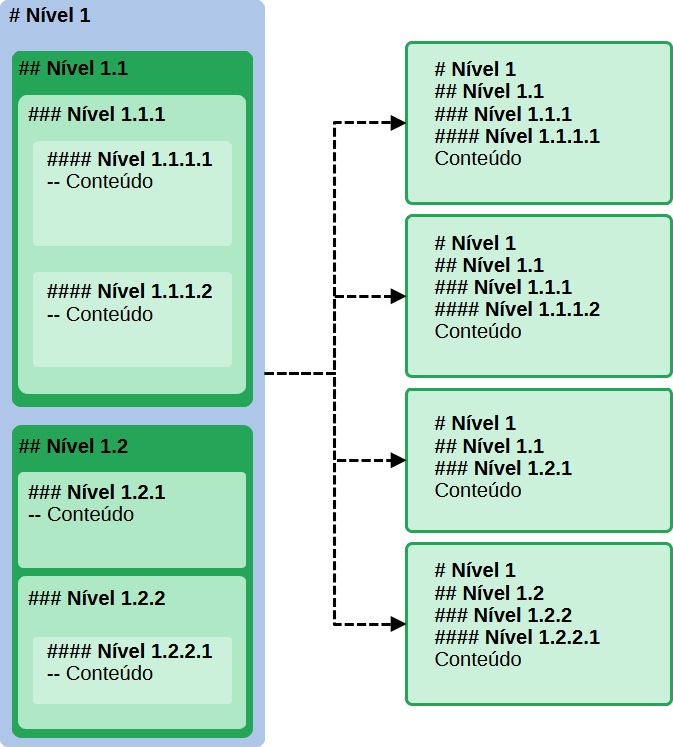
\includegraphics[width=0.5\linewidth]{Imagens/fragmentacao-hierarquico.png}
    \caption{Estratégia de Fragmentação de Arquivos Hierárquicos}
    Fonte: autoria própria
    \label{fig:fragmentacao-hierarquico}
\end{figure}

Assim, se aplicássemos essa abordagem sobre o exemplo de texto hierárquico que usamos anteriormente, o fragmento que contém a segunda seção chamada ``Como instalar o Ollama'' ficaria com o seguinte conteúdo:

    \begin{quote}
    {
        \begin{minipage}{\dimexpr\linewidth-2em}
        \setlength{\rightskip}{0.7em}
        \footnotesize
        \ttfamily
        \raggedright
        \sloppy
        Preparação do Ambiente
        
        Windows
        
        Como instalar o Ollama
        
        - Acesse a página de download do Ollama no link\\
        https://ollama.com/download/windows\\
        e faça o download do instalador.
        - Execute o instalador e siga as instruções em tela
        \end{minipage}
    }
    \end{quote}

Dessa forma, mantivemos indicadores explícitos que sinalizam a posição do fragmento dentro da estrutura geral do documento incorporados ao conteúdo textual da seção, aplicando algum grau de redução da dispersão de informação e perda de dados contextuais.

\section{Definindo o Banco Vetorial}
\label{sec:Metodologia.2}
Havendo sido separados os dados de interesse para a aplicação, era necessário organizar o banco vetorial (Seção \ref{sec:Assistente.1}) em que estes seriam representados, armazenados e disponibilizados às consultas. Dado que a opção feita foi pelo Chroma DB (Seção \ref{subsec:Assistente.1.1}), o qual se trata de um banco vetorial que, com fins de otimização de desempenho, opera ``em memória'', não carecendo de instalação no sentido estrito da palavra -- diferindo dos \ac{SGBD}s tradicionais --, bastando somente instalar a biblioteca Python disponibilizada pela Chroma, visto que utilizaremos essa linguagem de programação para integrar as partes/módulos do assistente (ver Seção \ref{sec:Metodologia.4}). Agora, portanto, tratamos dos aspectos de configuração do banco Chroma DB para, posteriormente, receber os dados que serão servidos nas buscas dos usuários.

\subsection{Escolhendo o modelo de Embeddings}
\label{subsec:Metodologia.2.1}
A Seção \ref{subsec:Assistente.1.2} apresentou a possibilidade de fornecer ao Chroma DB uma função de geração de \textit{embeddings} personalizada, permitindo escolher qual modelo de representação vetorial ser utilizado. Tratamos, nesse ponto do estudo, de definir, dentre um conjunto de modelos candidatos, qual teria o melhor desempenho em termos de recuperação de conteúdo relevante em relação à consulta feita. A seleção de modelos feita incluiu os seguintes modelos: (1) \textit{instructor-xl}, (2) \textit{text-embedding-ada-002} (ao qual nos referiremos como \textit{ada-002}, (3) \textit{text-embedding-3-large} (que nominaremos como \textit{3-large}), (4) \textit{GTE}, (5) \textit{BGE-m3}, (6) \textit{Llama3.1}, (7) \textit{DeepSeek-r1} e (8) \textit{BERT-QA}. Apresentamos, a seguir, cada um deles.

\subsubsection{instructor-xl}
\label{subsubsec:Metodologia.2.1.1}

Dentre os modelos avaliados, o que mais chamou atenção foi o \textit{instructor-xl} dada a sua proposta de flexibilidade. Trata-se de um modelo desenvolvido pela equipe de pesquisa de Processamento de Linguagem Natural (NLP) da Universidade de Hong Kong, incluindo a participação de pesquisadores de outras instituições, como \textit{University of Washington}, Meta AI e \textit{Allen Institute for AI}, publicado em 2023 \cite{Instructor:1}. O modelo selecionado pertence à série de modelos INSTRUCTOR, que são projetados para gerar \textit{embeddings} de texto de alta qualidade e se baseiam na arquitetura \textit{Transformer}, assim como modelos de estado da arte, como \ac{BERT} e \ac{GPT}.

No trabalho de  \citeonline{Instructor:2}, os seus publicadores o definem como \textit{``One Embedder [for] Any Task''} (Um Gerador de \textit{Embeddings} para Qualquer Tarefa) e como

\begin{citacao}
    \textit{an instruction-finetuned text embedding model that can generate text embeddings tailored to any task (e.g., classification, retrieval, clustering, text evaluation, etc.) and domains (e.g., science, finance, etc.) by simply providing the task instruction, without any finetuning.} \footnote{Um modelo de geração de \textit{embeddings} textuais com \textit{fine-tuning} feito a partir de uma instrução, capaz de gerar \textit{embeddings} de texto otimizados para qualquer tarefa (tais como, classificação, recuperação, agrupamento, avaliação de texto, etc.) e quaisquer domínios (quais sejam ciência, finanças, etc.) simplesmente fornecendo a instrução da tarefa, sem necessidade de \textit{fine-tuning} tradicional. (Tradução nossa)}
\end{citacao}

Os INSTRUCTORs são, portanto, modelos de criação de \textit{embeddings} textuais de forma adaptativa. Em vez de gerar \textit{embeddings} baseando-se unicamente nos parâmetros alcançados em seu treinamento, ele lança mão de instruções em linguagem natural fornecidas no momento de sua execução, as quais devem descrever as tarefas em que os \textit{embeddings} serão utilizados. Ao utilizar as instruções como elementos ``direcionadores'' do processo de geração de \textit{embeddings}, pretende-se que o resultado final seja otimizado para as tarefas definidas, fazendo as vezes de um ``ajuste fino''. Essa abordagem demonstra, segundo os seus desenvolvedores, bom desempenho em não somente ``compreender'' texto em um sentido mais aberto e genérico, sendo capaz, também, de interpretá-lo com uma visão direcionada a aplicações e casos de uso particulares.

Desta forma, as representações vetoriais geradas são otimizadas para tarefas específicas (como classificação, recuperação de informações, agrupamento, avaliação semântica, entre outras) e/ou domínios diferentes, sem a necessidade de refinamento do modelo nos moldes tradicionais de \textit{finetuning}, tornando-o adaptável e mais relevante para diversas aplicações.
A versão do modelo que escolhemos testar para possível uso no Assistente de Busca, especificamente, é a \textit{instructor-xl}, sendo a variante dentre a família de modelos INSTRUCTOR com maior tamanho, otimizada para desempenho e equilíbrio entre precisão e eficiência em aplicações de \ac{PLN}, podendo ser utilizada por meio do \textit{framework} \textit{sentence-transformer}, disponibilizado pelo \textit{HuggingFace}, como \textit{hkunlp/instructor-xl}.

\subsubsection{text-embedding-ada-002}
\label{subsubsec:Metodologia.2.1.2}

Outro modelo selecionado por ser promissor foi o \textit{text-embedding-ada-002}, desenvolvido e oferecido como um serviço pela OpenAi desde o final do ano de 2022. A página de apresentação do modelo o descreve como a unificação de cinco modelos anteriores (\textit{text-similarity}, \textit{text-search-query}, \textit{text-search-doc}, \textit{code-search-text} and \textit{code-search-code}) em um único modelo aprimorado, alcançando melhores resultados em busca textual, similaridade de frases e \textit{benchmarking} de busca em código \cite{ADA:1}.

Um dos pontos positivos apontados na página é o fato de utilizar uma forma compacta de representação em \textit{embeddings} (apenas 1.536 dimensões), apresentando melhor custo-benefício para utilização em bancos vetoriais, a despeito do suporte a um contexto maior. A isso adiciona-se o fato de ser menos computacionalmente custoso de se utilizar, dado que o processamento é delegado à API da OpenAI, enviando o texto a ser processado, via requisição HTTP e recebendo os \textit{embeddings} como resposta.

Como ponto negativo há o custo atrelado a cada requisição feita à API, tanto para gerar os \textit{embeddings} dos documentos quanto, posteriormente, para gerar os \textit{embeddings} de cada consulta feita ao banco de vetores, enquanto houver utilização da aplicação.

Embora não seja o modelo mais recente, dado que outros modelos mais eficientes e comparativamente baratos hajam sido lançados pela OpenAi, o posicionamento da empresa é de que o \textit{ada-002} não está sendo declarado como obsoleto (\textit{deprecated}) de forma que, embora recomendem o \textit{text-embedding-3-large}, seu modelo mais novo (ver a Seção \ref{subsubsec:Metodologia.2.1.3}), os clientes podem continuar usando o \textit{ada-002}.\footnote{``We are not deprecating text-embedding-ada-002, so while we recommend the newer model, customers are welcome to continue using the previous generation model'' \cite{3_large:1}.}

\subsubsection{text-embedding-3-large}
\label{subsubsec:Metodologia.2.1.3}

Lançado em janeiro de 2024, o modelo \textit{text-embedding-3-large}, juntamente com o \textit{text-embedding-3-small}, representa uma nova geração de modelos de vetorização textual desenvolvidos pela OpenAI, caracterizando-se por sua maior capacidade e desempenho superior em tarefas de representação semântica. Este modelo é capaz de gerar \textit{embeddings} com até 3.072 dimensões, o que possibilita uma codificação mais rica e detalhada de textos em espaços vetoriais de alta dimensionalidade.

O modelo \textit{text-embedding-3-large} apresenta desempenho substancialmente superior ao \textit{text-embedding-ada-002}, com destaque para os ganhos observados nos \textit{benchmarks} MIRACL (de 31,4\% para 54,9\%) e MTEB (de 61,0\% para 64,6\%), indicando avanços consistentes na qualidade dos \textit{embeddings} em tarefas de recuperação de informações, similaridade semântica, classificação e ranqueamento.

A adoção do \textit{text-embedding-3-large} é, portanto, recomendada para aplicações que exigem representações vetoriais de alta fidelidade, particularmente em contextos multilíngues e domínios que demandam precisão semântica elevada.


\subsubsection{GTE}
\label{subsubsec:Metodologia.2.1.4}
Desenvolvida pela \textit{Aliyun} ou \textit{Alibaba Cloud}, uma das subsidiárias do conglomerado chinês Alibaba Group voltada para o mercado de computação em nuvem, a série de modelos \textit{GTE-Multilingual} (\textit{mGTE}) -- uma reformulação do \textit{General Text Embedding} (\textit{GTE}) -- foi apresentada em novembro de 2024. A empresa aponta que o conjunto de modelos

\begin{citacao}
    \textit{offers high performance, long-context handling, multilingual support, and elastic embedding, significantly improving retrieval and ranking efficiency (...) [being, therefore,] suitable for a wide range of advanced \ac{RAG} applications} \cite{GTE:1}.
    \footnote{oferece um alto desempenho, tratamento de contextos longos, suporte multi-idiomas e \textit{embeddings} com tamanho ajustável, aprimorando significativamente a eficiência na recuperação e re-rankeamento/reclassificação, (...) [sendo, portanto,] adequadas ao uso em uma ampla gama de aplicações avançadas de \ac{RAG}. (Tradução nossa)}
\end{citacao}

O conjunto inclui ``modelos base, modelos de \textit{embeddings} e de \textit{ranking}'' \cite{GTE:1}, com resultados promissores particularmente para tarefas de recuperação de documentos, sendo amplamente utilizados como modelos de referência por organizações como a PostgresML \cite{GTE:2}. Dado que em sua própria documentação e material de divulgação dos modelos o \textit{mGTE} é referido simplesmente como \textit{GTE}, adotaremos aqui a mesma nomenclatura.

Assim como com o \textit{instructor-xl}, também é possível utilizar o \textit{GTE} com o \textit{sentence-transformer}, como \textit{Alibaba-NLP/gte-multilingual-base}.

\subsubsection{BGE-m3}
\label{subsubsec:Metodologia.2.1.5}
O \textit{BGE-m3} é um modelo desenvolvido por pesquisadores da \textit{Beijing Academy of Artificial Intelligence} -- BAAI (uma organização de pesquisa em inteligência artificial, sem fins lucrativos, também conhecida como \textit{Zhiyuan Institute}) e da \textit{University of Science and Technology of China}. Os autores o apontam como um modelo distinto dos demais em termos de versatilidade, considerando três frentes distintas: multilinguística, multifuncionalidade e multigranularidade.

Apontam \citeonline{BGE:1} que o \textit{M3-Embedding} foi capaz de abstrair um ``espaço semântico comum'' a todas as línguas sobre as quais foi feito o processo de treinamento, permitindo-lhe demonstrar competência na recuperação de conteúdo semanticamente semelhante com suporte a mais de 100 idiomas. Adicionalmente, dado que sua representação interna é feita sobre essa camada semântica abstrata compartilhada, é possível realizar recuperação de conteúdo interlinguístico.

No que concerne a multifuncionalidade e multigranularidade,

\begin{citacao}
    \textit{[M3-Embedding] is able to generate versatile embeddings to support different retrieval functionalities, not just dense retrieval, but also sparse retrieval and multivector retrieval. Finally, M3-Embedding is learned to process different input granularities, spanning from short inputs like sentences and passages, to long documents of up to 8,192 input tokens.} \cite{BGE:1}
    \footnote{[O \textit{M3-Embedding}] é capaz de gerar \textit{embeddings} versáteis que viabilizam múltiplas funcionalidades de recuperação da informação, abrangendo não apenas a recuperação densa, mas também a recuperação esparsa e a recuperação por multivetores. Por fim, o \textit{M3-Embedding} é treinado para lidar com diferentes granularidades de entrada, variando desde entradas curtas, como frases e excertos, até documentos extensos, com até 8.192 \textit{tokens} de entrada. (Tradução nossa)}
\end{citacao}

O modelo também é utilizável a partir do \textit{framework} do HuggingFace como \textit{BAAI/BGE-m3}, tornando simples a sua utilização no projeto.

\subsubsection{Outros Modelos}
\label{subsubsec:Metodologia.2.1.6}
Durante o processo de escolha dos modelos a serem usados na função para gerar os \textit{embeddings} a serem utilizados no banco vetorial, apercebemo-nos de que a ferramenta Ollama (abordada na Seção \ref{subsec:Assistente.2.3}, de cujos detalhes de implementação trata a Seção \ref{sec:Metodologia.3}) possui a funcionalidade de utilização de modelos diversos para geração de \textit{embeddings}. Dado que já incluíramos \ac{LLM}s na ferramenta, decidimos incluí-los no conjunto de modelos a serem testados para geração de representações vetoriais na aplicação.

Ademais, quando da análise exploratória de abordagens do problema objeto deste estudo, encontramos modelos treinados especificamente para utilização em aplicações de perguntas e respostas (\textit{Q\&A Systems}), de forma que, na fase de realização de testes de desempenho dos modelos, já estava um deles disponível nos dispositivos de execução do projeto. Sendo esse modelo específico capacitado à geração de \textit{embeddings}, optamos por também incluí-lo no rol de modelos a serem avaliados.

É importante notar, todavia, que os \ac{LLM}s e o modelo com ajuste fino para Q\&A recém mencionados são otimizados para tarefas distintas da geração de representações vetoriais de texto, os \textit{embeddings} necessários para utilização no banco vetorial. Logo, é até esperado que alcancem resultados consideravelmente aquém dos alcançado por modelos como o \textit{ada-002}, o \textit{3-large}, o \textit{instructor-xl}, o \textit{GTE} e o \textit{BGE-m3}, com um foco maior na geração de \textit{embeddings} voltados à recuperação de conteúdo por similaridade semântica. A opção por sua inclusão em meio aos modelos especializados se restringe a fins de comparação e curiosidade.

Temos, portanto, os seguintes modelos adicionais:

\begin{itemize}
    \item \textbf{Llama3.1:latest}: modelo que detalhado na Seção \ref{subsec:Assistente.2.1}, desenvolvido pela Meta AI. Trata-se de um \ac{LLM}, por natureza otimizado para geração de texto. Será utilizado por meio da ferramenta Ollama (Seção \ref{subsec:Assistente.2.3}).
    \item \textbf{DeepSeek-r1:7b}: modelo destilado do \textit{DeepSeek-r1}, da DeepSeek, baseado na arquitetura \textit{qwen2}, detalhado na Seção \ref{subsec:Assistente.2.2} Também se trata de um \ac{LLM}, sendo a geração de texto seu fim principal. Assim como no caso do \textit{Llama3.1}, lançaremos mão da ferramenta Ollama para utilizar o modelo.
    \item \textbf{bert-base-cased-squad-v1.1-portuguese} (\textit{BERT-QA}): baseado no modelo \textit{BERTimbau Base} (uma versão do \textit{BERT} pré-treinada para português do Brasil, desenvolvida pela Neuralmind.ai), este modelo teve um ajuste fino para utilização em aplicações de perguntas e respostas (\textit{Q\&A Systems}) -- para isso utilizando uma versão em português do \textit{Stanford Question Answering Dataset} (\textit{SQuAD}) \cite{BERT_QA:1}.
\end{itemize}

\subsubsection{Limitações de Tamanho de Entrada}
\label{subsubsec:Metodologia.2.1.7}

Modelos de geração de \textit{embeddings} possuem restrições quanto ao número máximo de \textit{tokens} que são capazes de processar por cada entrada de texto a ser vetorizado, uma limitação que afeta diretamente o volume de texto sobre o qual o modelo pode ser aplicado. Conhecer a capacidade de cada modelo é essencial para definir estratégias de segmentação de documentos, especialmente diante da possibilidade de tratamento de textos longos.

A Tabela~\ref{tab:num-maximo-tokens} apresenta o número máximo de \textit{tokens} suportado pelos modelos apresentados na seção anterior. Modelos baseados na arquitetura \textit{BERT} ou variantes similares (como \textit{GTE}, \textit{BGE-m3}, \textit{instructor-xl} e \textit{BERT-QA}) geralmente suportam até 512 \textit{tokens}, o que exige particionamento cuidadoso de textos longos. Por outro lado, modelos mais recentes e robustos, como os da família \textit{Llama} e \textit{DeepSeek}, além dos modelos proprietários da OpenAI (\textit{ada-002} e \textit{3-large}), oferecem suporte para entradas significativamente maiores, com capacidade próxima ou superior a 8.000 \textit{tokens}.

\begin{table}[H]
    \caption{Especificações dos Modelos de \textit{Embeddings}}
    \centering
    \begin{tabular}{ l r r }
        \hline
        \textbf{Modelo} & \textbf{Número Máximo de \textit{Tokens}} & \textbf{Tamanho do Vetor} \\  
        \hline
        \textit{GTE} & 8.192 & 768 \\
        \textit{BGE-m3} & 8.192 & 1.024 \\
        \textit{instructor-xl} & 512 & 768 \\
        \textit{BERT-QA} & 512 & 768 \\
        \textit{Llama3.1} & $\geq 130.000$ & 4.096 \\
        \textit{DeepSeek-r1:7b} & $\approx 32.768$ & 3.584 \\
        \textit{ada-002} (OpenAI) & 8.191 & 1.536 \\
        \textit{3-large} (OpenAI) & 8.191 & 3.072 \\
        \hline
    \end{tabular}
    
    Fonte: O autor (2025)
    \label{tab:num-maximo-tokens}
\end{table}

Além da qualidade das representações geradas pelos modelos, suas limitações quanto à vetorização texto mais extenso sem necessidade de truncamento devem ser levadas em consideração. Como apontado na Seção \ref{subsec:Metodologia.1.1}, considerando que as unidades básicas de informação autocontidas, no contexto de peças legislativas selecionadas, (os artigos), em sua grande maioria, são pequenos o suficiente para respeitar o limite de 512 \textit{tokens}, todos os modelos a serem avaliados têm suporte para realizar a geração de seus \textit{embeddings}.


\subsection{Exploração Inicial da Qualidade dos \textit{Embeddings} Gerados}
\label{subsec:Metodologia.2.2}

Como uma forma de realizar uma exploração inicial da qualidade dos \textit{embeddings} gerados por cada um dos modelos, os utilizaremos para gerar representações vetoriais de um conjunto de documentos textuais de naturezas variadas, cujos \textit{embeddings} nos servirão como recurso para realizar as avaliações.

O conjunto de dados em questão utiliza uma seleção de excertos textuais com conteúdo pertinente a diversas áreas e temas:

\begin{enumerate}
    \item \textbf{\texttt{apocrifo.txt}}: texto da tradução em português do livro apócrifo ``O Evangelho de Judas'';
    \item \textbf{\texttt{cabala.txt}}: texto em português do livro que trata de iniciação à Cabala (``Um Guia à Sabedoria Oculta da Cabala'');
    \item \textbf{\texttt{codigo\_penal.txt}}: texto original do código penal brasileiro;
    \item \textbf{\texttt{comunismo.txt}}: texto do ``Manifesto Comunista'', por Karl Marx e Friedrich Engels;
    \item \textbf{\texttt{culinaria.txt}}: seleção de partes do livro ``Todas as Técnicas de Culinária'', por Jeni Wright e Eric Treuille;
    \item \textbf{\texttt{fisica.txt}}: seleção de partes de um livro de física para o ensino médio;
    \item \textbf{\texttt{historia.txt}}: seleção de partes do texto historiográfico A escravidão no ``Seridó'', por Helder Alexandre Medeiros de Macedo;
    \item \textbf{\texttt{regimento\_alern.txt}}: texto completo do Regimento Interno da Alern.
\end{enumerate}

Os documentos serão fragmentados de forma simples, sendo divididos em conjuntos de orações completas, limitados ao comprimento máximo de 500 palavras, após o que serão vetorizados utilizando cada um dos modelos de geração de \textit{embeddings} apresentados na Seção \ref{subsec:Metodologia.2.1}, sendo o resultado armazenado para realização das análises a que nos propomos. Essa exploração consiste em utilizar os \textit{embeddings} para (1) utilizar como dados de treinamento para um classificador simples -- de forma a considerar a eficiência dos modelos em capturar as especificidades semânticas de cada um dos temas abordados pelos documentos; e (2) realizar particionamento do conjunto de dados em \textit{clusters} -- como forma de avaliar o quão bem cada modelo consegue capturar a similitude/discrepância entre fragmentos de documentos abordando temas diversos.

Adicionalmente, realizaremos a comparação dos \textit{embeddings} gerados em dois contextos, cada um correspondendo a um dos seguintes conjuntos de documentos:

\begin{itemize}
    \item \textbf{Conjunto de documentos 1} — análise de um conjunto de documentos com \textit{estilos, formas e conteúdos distintos}, utilizando os arquivos: \texttt{apocrifo.txt}, \texttt{cabala.txt}, \texttt{comunismo.txt}, \texttt{culinaria.txt}, \texttt{fisica.txt}, \texttt{historia.txt} e \texttt{regimento\_al.txt};
    \item \textbf{Conjunto de documentos 2} — justaposição de documentos com \textit{estilos e formas semelhantes, porém com conteúdo diverso}, utilizando os arquivos: \texttt{regimento\_al.txt} e \texttt{cod\_penal.txt}.
\end{itemize}

Com o objetivo de obter uma intuição visual mais clara acerca da similaridade ou dissimilaridade entre os arquivos utilizados em cada conjunto de dados, realizaremos uma representação gráfica dos \textit{embeddings} gerados por cada modelo. Para isso, aplicaremos uma técnica de redução de dimensionalidade, uma vez que os \textit{embeddings} operam em espaços vetoriais de alta dimensão, o que inviabiliza sua visualização direta. A técnica escolhida foi \textit{\ac{TSNE}} \cite{TSNE}, que preserva, de forma eficaz, tanto a estrutura local quanto a estrutura global dos dados em espaços de menor dimensão. Assim, ao projetarmos os vetores em um espaço bidimensional, conseguimos observar visualmente como os documentos se agrupam ou se separam com base em suas características semânticas. Essa representação imagética permite uma análise exploratória complementar, possibilitando identificar padrões de proximidade, dispersão ou sobreposição entre as diversas representações dos documentos por \textit{embeddings}.

Para a avaliar (somente de forma exploratória, sem intuito de otimização) o comportamento dos modelos sobre dados com estilos distintos com classificação, empregaremos um classificador simples, utilizando o algoritmo \textit{Random Forest} -- por meio da classe \texttt{RandomForestClassifier} disponível na biblioteca \texttt{sklearn.ensemble}, instanciada com seus valores padrão e usando \texttt{n\_estimators=100}. Após o treinamento, a avaliação do desempenho preditivo do classificador será realizada utilizando duas métricas: acurácia e coeficiente de correlação de Matthews (MCC), bem como F1-Score Macro e Ponderado.

De forma a avaliar o comportamento dos modelos sobre textos com mesmo estilo, mas conteúdo diverso usando \textit{clustering} sobre as representações vetoriais geradas, utilizaremos os algoritmos de particionamento \textit{K-Means}, implementado pela função \texttt{KMeans} do módulo \texttt{sklearn.cluster}, e DBSCAN, com implementação por \texttt{sklearn.cluster.DBSCAN}. Neste experimento, como aprioristicamente sabemos a quantidade de partições (documentos com temas bem definidos) o valor de \textit{k} será fixado em \textit{7} para o Conjunto de Documentos 1 e \textit{2} para o Conjunto de Documentos 2.

Para avaliar a qualidade das partições, foram utilizadas duas métricas internas:

\begin{itemize}
    \item \textbf{Índice de Silhueta (\textit{Silhouette})}: mensura o quão próximo cada ponto está posicionado em relação aos outros pontos de sua partição em comparação com os pontos nas partições vizinhas. O valor varia entre \textit{–1} e \textit{1}. Valores próximos de \textit{1} indicam que os pontos estão bem agrupados com os seus semelhantes (alta coesão) e distantes de outras partições (boa separação).

    \item \textbf{Índice de Davies-Bouldin (DB}): avalia a qualidade do particionamento com base na dispersão interna dos pontos de uma partição e na distância entras partições. É calculado como a média das razões entre a dispersão intra-partição e a separação inter-partições. Valores mais baixos indicam \textit{clusters} mais compactos e melhor separados, ou seja, uma clusterização de maior qualidade.
\end{itemize}

Assim, aferindo a coesão intra-partição e a separação inter-partições, é possível comparar de forma objetiva a capacidade de organização semântica dos diferentes modelos de \textit{embedding}. A coesão serve como um indicador representativo do quão bem cada modelo consegue identificar assuntos de um tema específico (similarmente ao que a etapa de classificação realizada anteriormente sugere), ao passo que a separação pode ser usada como uma medida substituta para avaliar o quanto o modelo gera \textit{embeddings} que confundem assuntos distintos como correlatos.

Consideradas essas intuições iniciais sobre os modelos de \textit{embeddings}, serão feitas avaliações sobre seu desempenho no contexto de recuperação de conteúdo por meio das aferições de resultados com outros conjuntos de dados e por meio de outros métodos e métricas. Esse processo será executado conforme disposto na Seção \ref{sec:Metodologia.6}, em especial na Seção \ref{subsec:Metodologia.6.1}, com os resultados expostos na Seção \ref{subsec:Resultados.2.1}.

\subsection{Ingestão de Dados no Banco Vetorial}
\label{subsec:Metodologia.2.3}

A inclusão dos documentos no banco vetorial, o Chroma DB, em forma de seus fragmentos, foi realizada utilizando as ferramentas de manipulação do banco, de forma direta e simples, sem utilização de \textit{frameworks} ou bibliotecas de terceiros. A estrutura de cada fragmento inserido possui, além do conteúdo textual, algumas outras informações que podem ser utilizadas a posteriori.

A estrutura final de cada uma das entradas no Chroma DB se configura como se segue:
\begin{itemize}
    \item \texttt{id}: identificador único da entrada (fragmento)
    \item \texttt{page\_content}: texto original do fragmento
    \item \texttt{metadata}: metadados com informações relevantes a respeito do fragmento, bem como do documento como um todo, incluindo:
    \begin{itemize}
        \item \texttt{título}: O título do documento original
        \item \texttt{subtítulo}: O número do artigo e indicador nos casos de subdivisão de conteúdo
        \item \texttt{autor}: Entidade/sujeito autor do documento
        \item \texttt{fonte}: Link para o arquivo de origem do documento
    \end{itemize}
\end{itemize}

Como uma peculiaridade do Chroma DB, há o fato de que o id de cada entrada inserida é informado no momento da inserção, não sendo algo que o banco vetorial se encarrega de realizar. Semelhantemente, os elementos dos metadados são definidos, tanto em seus campos quanto em seu conteúdo, de forma flexível, ao se inserir um documento (fragmento, no caso presente) em uma coleção. Destarte, é possível incluir campos de controle adicionais, de forma a interligar fragmentos co-dependentes (como no caso de artigos segmentados por terem um tamanho maior que o número máximo de palavras definido).

A etapa principal da inclusão de documentos em um banco vetorial consiste na geração e persistência da representação vetorial de cada documento/fragmento, para o que é necessária a utilização de uma função de geração de \textit{embeddings}. Considerando que é necessário analisar a qualidade dos resultados de consulta utilizando os modelos que optamos por avaliar (ver Seção \ref{subsec:Assistente.1.2}), dentro do mesmo banco vetorial criamos um conjunto de coleções, cada uma das quais utilizando um dos modelos propostos em sua função de geração de vetores de \textit{embeddings} para ser aplicada nos fragmentos. As coleções criadas e os modelos utilizados em cada uma são apresentados na Tabela \ref{tab:colecoes-modelos-embeddings}.

\begin{table}[H]
    \caption{Coleções e Modelos no Banco Vetorial de Testes}
    \centering
    \begin{tabular}{ l l }
        \hline
        \textbf{Coleção} & \textbf{Modelo Utilizado} \\  
        \hline
        \texttt{documentos\_rh\_bge\_m3} & \textit{BAAI/BGE-m3} \\
        \texttt{documentos\_rh\_openai} & \textit{text-embedding-ada-002} \\
        \texttt{documentos\_rh\_alibaba} & \textit{Alibaba-NLP/gte-multilingual-base} \\
        \texttt{documentos\_rh\_instructor} & \textit{hkunlp/instructor-xl} \\
        \texttt{documentos\_rh\_bert\_pt} & \textit{pierreguillou/bert-base-cased-squad-v1.1-portuguese} \\
        \texttt{documentos\_rh\_deepseek} & \textit{deepseek-r1:7b} \\
        \texttt{documentos\_rh\_llama} & \textit{Llama3.1} \\
        \hline
    \end{tabular}   
    
    Fonte: O autor (2025)
    \label{tab:colecoes-modelos-embeddings}
\end{table}

Após a inclusão, os documentos são passíveis de serem recuperados em consultas realizadas junto ao banco vetorial, com base na sua similaridade semântica com uma pergunta ou critério de busca definidos. Assim, as solicitações realizadas ao Chroma DB estão definidas de forma tal a recuperar os \textit{n} documentos mais relevantes, ordenados de forma decrescente pelo grau de similaridade com a pergunta utilizada como critério de consulta.

\section{Configuração do LLM}
\label{sec:Metodologia.3}
A configuração dos modelos geradores de texto a serem testados e comparados, visto que foi feita a opção pelo uso do Ollama como meio de simplificar o processo, se deu de forma direta. Os arquivos de instalação do Ollama foram obtidos e executados diretamente da sua página de download \cite{Ollama:2}. Após a instalação, foi realizada a inclusão dos modelos selecionados (ver Seção \ref{sec:Assistente.2}), propriamente ditos, tornando-os disponíveis para utilização.

Ao considerar as versões disponíveis dos modelos \textit{Llama} e \textit{DeepSeek}, levamos em consideração as limitações de recursos nas máquinas disponíveis, buscando dentre os modelos mais atuais opções robustas o suficiente para oferecer bons resultados, sem, contudo, necessitar de recursos para além dos disponíveis. Com isto, optamos pelas seguintes versões:

\begin{itemize}
    \item \textbf{Llama:} \textit{Llama3.1:8b}
    \item \textbf{DeepSeek:} \textit{DeepSeek-r1:7b} (destilado a partir do DeepSeek-V2.5/V3 sobre o \textit{qwen2})
\end{itemize}

Embora haja as versões mas recentes (\textit{Llama} 3.2 e 3.3) ou mais robustas (\textit{DeepSeek-r1} com 70B), elas são disponibilizadas  ou em tamanhos muito pequenos (tais como o \textit{Llama3.2:1b}), com resultados sub-ótimos para nossos recursos, ou em tamanhos demasiadamente grandes, extrapolando as limitações de \textit{hardware} disponível. 

O Ollama disponibiliza a geração de respostas do modelo por meio de uma API REST, se encarregando de fazer o gerenciamento dos recursos disponíveis para a otimização do processo. As requisições feitas à API apontam o modelo específico a ser utilizado (no caso de nossos testes, o \textit{Llama3.1} ou o \textit{DeepSeek-R1}); uma mensagem de sistema, que se encarrega de estabelecer a forma que o modelo deve seguir para gerar as respostas;  o histórico de mensagens trocadas entre o usuário e a API em interações anteriores; e o \textit{prompt} em si, o qual contém tanto o conteúdo recuperado do banco vetorial, quanto a consulta do usuário. Ademais, acrescenta-se a configuração que determina se a resposta deve ser enviada \textit{token} a \textit{token}, à medida que é gerada, ou de forma inteiriça, com todo o conteúdo gerado sendo disponibilizado quando do término de sua produção pelo \ac{LLM}.

\begin{figure}[H]
    \centering
    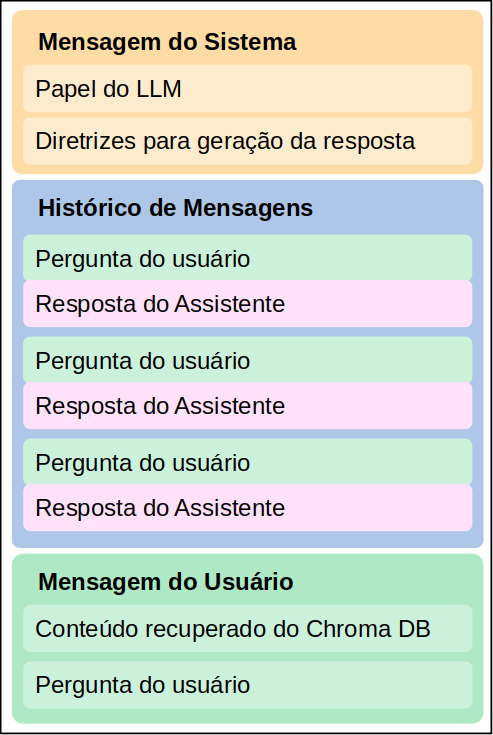
\includegraphics[width=0.5\linewidth]{Imagens/pilha-mensagem-ollama.png}
    \caption{Estrutura da mensagem enviada ao Ollama}
    Fonte: autoria própria
    \label{fig:pilha-mensagem-ollama}
\end{figure}


De forma a direcionar o comportamento dos \ac{LLM}s na geração das respostas, cada requisição feita à API utiliza uma mensagem de sistema fixa, bem como um modelo de \textit{prompt} com uma estrutura pré-definida (ver Figura \ref{fig:pilha-mensagem-ollama}), alterando somente a pergunta feita e o teor dos documentos em que a resposta deve se basear. Assim, os dados enviados à API têm a seguinte estrutura:

\begin{itemize}
    \item \textbf{Papel do \ac{LLM}}: Definição do papel que o modelo deve assumir, cujo teor é  
    \begin{quote}
    {
        \footnotesize
        \ttfamily
        \raggedright
        \sloppy
        ``Alern e ALRN significam Assembleia Legislativa do Estado do Rio Grande do Norte.
        
        Você é um assistente que responde a dúvidas de servidores da Alern sobre o regimento interno da Alern, o regime jurídico dos servidores estaduais do RN, bem como resoluções da Alern.
        
        Assuma um tom formal, porém caloroso, com gentileza nas respostas.
        
        Utilize palavras e termos que sejam claros, autoexplicativos e linguagem simples, próximo do que o cidadão comum utiliza.
        
        Responda utilizando o mesmo idioma em que a pergunta foi feita.'';
    }
    \end{quote}
    \item \textbf{Diretrizes de Geração}: Orientações a serem seguidas pelo \ac{LLM} na geração da resposta, sendo afixado como

        \begin{quote}
        {
        \begin{minipage}{\dimexpr\linewidth-2em}
        \setlength{\rightskip}{0.7em}
        \footnotesize
        \ttfamily
        \raggedright
        \sloppy
        ``Responda utilizando o mesmo idioma que foi usado na pergunta.
        
        Use as informações dos DOCUMENTOS fornecidos para gerar uma resposta clara para a PERGUNTA.
        
        Na resposta, não mencione que foi fornecido documentos de referência.
        
        Cite os nomes dos DOCUMENTOS e números dos artigos em que a resposta se baseia.
        
        A resposta não deve ter saudação, vocativo, nem qualquer tipo de introdução que dê a entender que houve interação anterior.
        
        As respostas dadas devem ser específicas para a pergunta atual, usando o histórico somente para fim de contexto.
        
        Se você não souber a resposta, assuma um tom gentil e diga que não tem \\ informações suficientes para responder.
        
        Caso a pergunta seja sobre temas que não envolvam busca de informação na documentação da Alern, educadamente se recure a responder. Em nenhuma circunstância escreva texto que incite violência ou comportamento criminoso e inadequado.'';
        \end{minipage}
        }
        \end{quote}
    \item \textbf{Histórico}: uma lista com o teor das mensagens trocadas anteriormente entre o usuário e o assistente. Dado que cada \ac{LLM} possui uma limitação no número máximo de \textit{tokens} dos \textit{prompts} por eles processados, apenas uma fração do conteúdo recebido pelo \ac{LLM} é incluída no histórico, sendo correspondente às 5 mais recentes interações do usuário com o assistente -- cinco pares pergunta-resposta. Nesse recorte, não estão contidos os conteúdos recuperados do banco vetorial (os quais serviram de base para a geração da resposta do Assistente), de sorte que apenas as perguntas feitas pelos usuários e as respostas dadas pela ferramenta são mantidas no histórico.
    
    \item \textbf{\textit{Prompt} do usuário}: texto formado pelo conteúdo dos documentos a serem utilizados para a geração da resposta e pela pergunta a ser respondida pelo \ac{LLM}. A Figura \ref{fig:prompt-usuario} mostra um exemplo de um \textit{prompt} em seu formato final.
\end{itemize}

\begin{figure}[H]
    \centering
    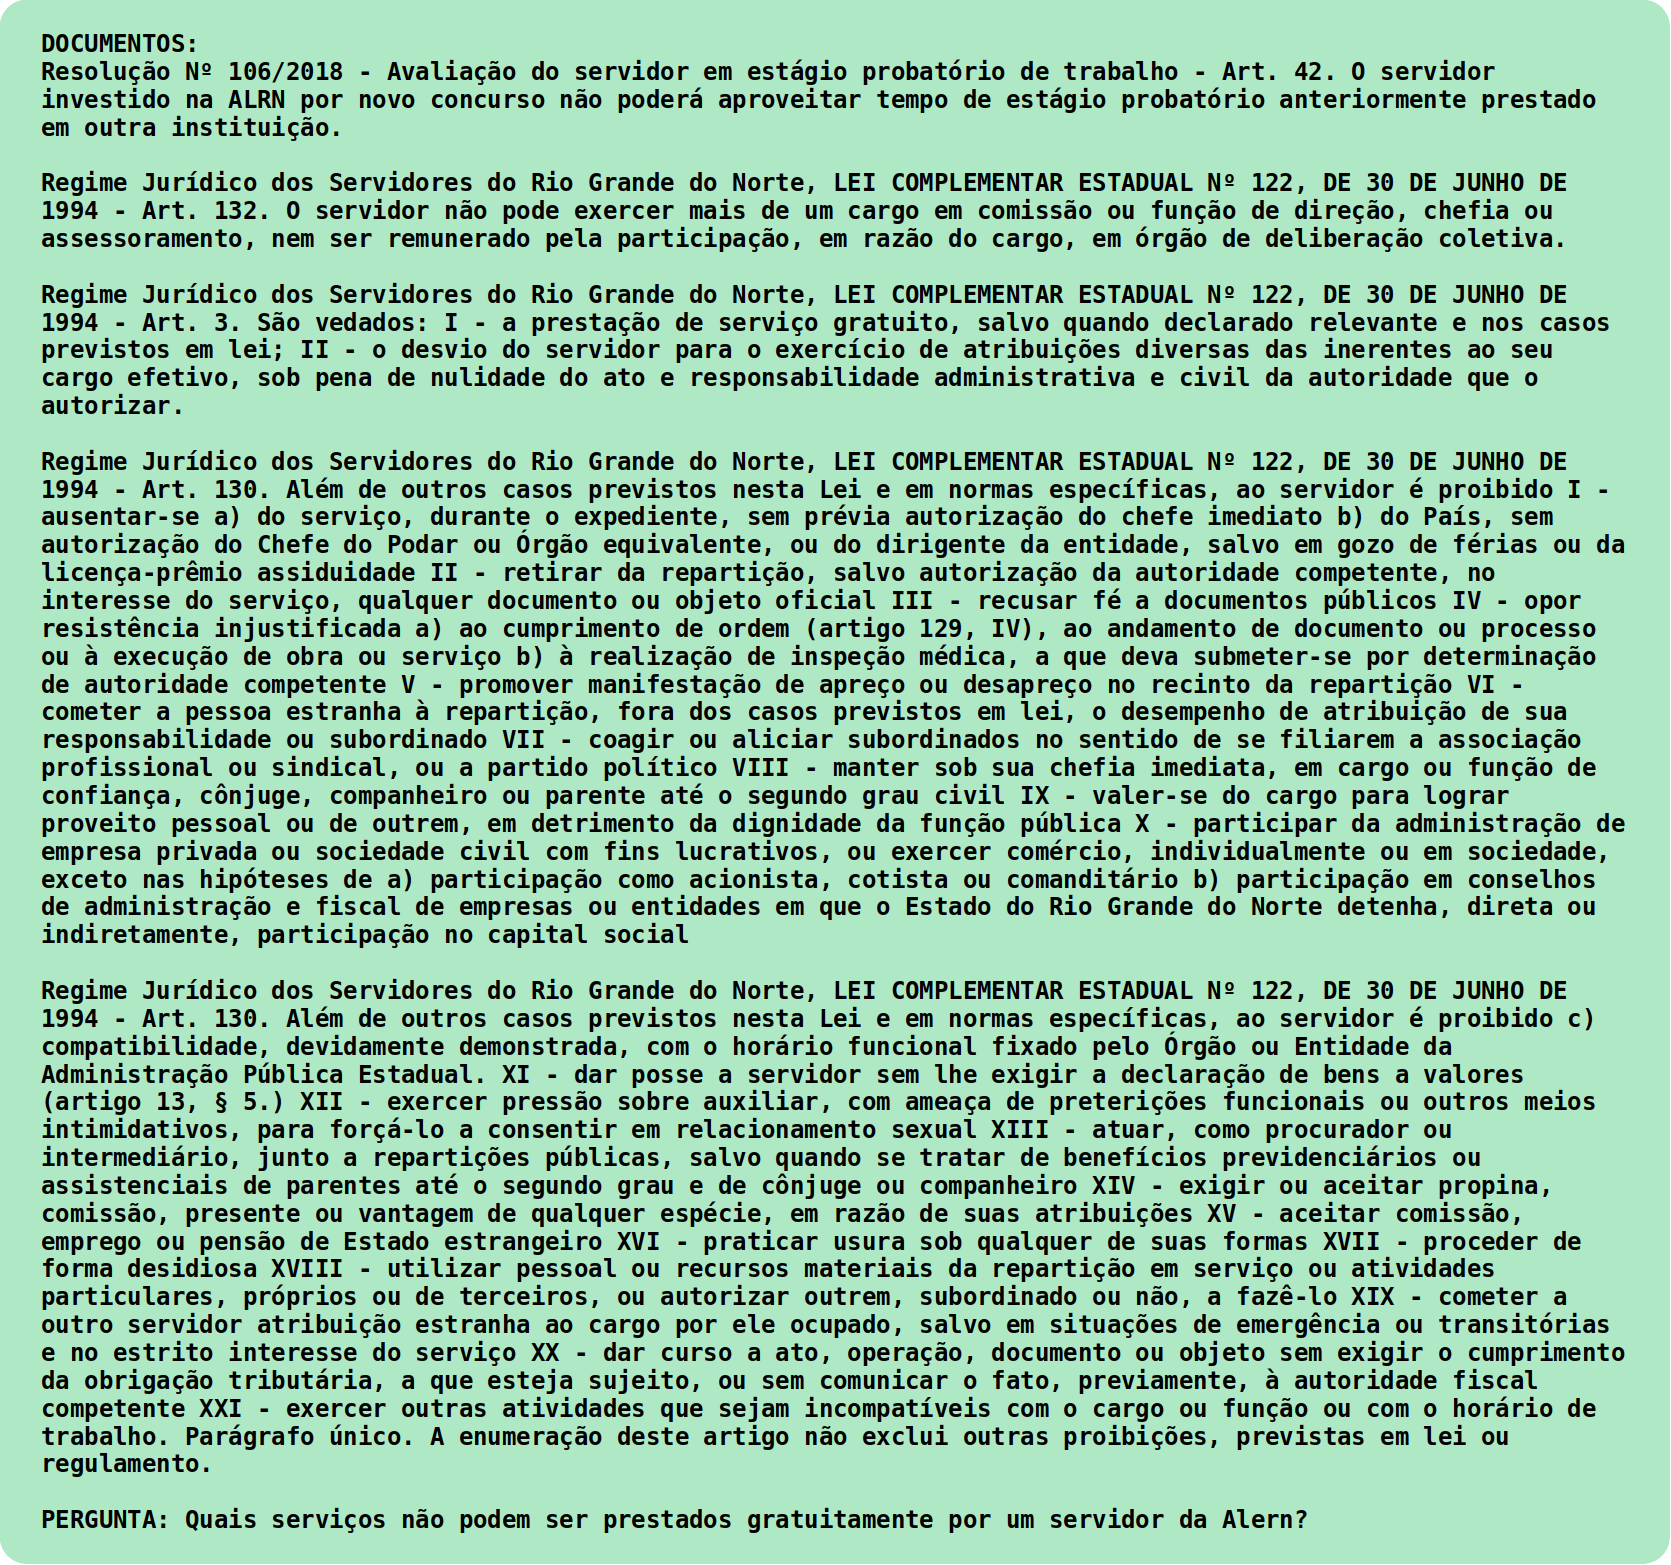
\includegraphics[width=1\linewidth]{Imagens/prompt-usuario.png}
    \caption{Estrutura do \textit{prompt} de usuário}
    Fonte: autoria própria
    \label{fig:prompt-usuario}
\end{figure}

\section{API Gerenciadora de Fluxo}
\label{sec:Metodologia.4}

A integração de todos os serviços oferecidos pelas camadas mencionadas é realizada por uma API gerenciadora de fluxo (utilizando a biblioteca FastAPI, na linguagem Python), que se encarrega de receber requisições de alguma interface de usuário, com as perguntas a serem utilizadas como critérios de consulta e acionar os serviços das outras camadas para a geração da resposta. Após receber os dados resultantes de cada um dos serviços nas fases intermediárias do processo inteiro, eles são formatados e preparados para serem direcionados ao elemento seguinte, até, finalmente, encaminhar à interface de usuário o produto final, na forma de uma resposta, com uma lista de documentos que lhe dão suporte.

A Figura \ref{fig:diag-atividade-assist-busca} demonstra o fluxo inteiro do processo como um todo.

\begin{figure}[H]
    \centering
    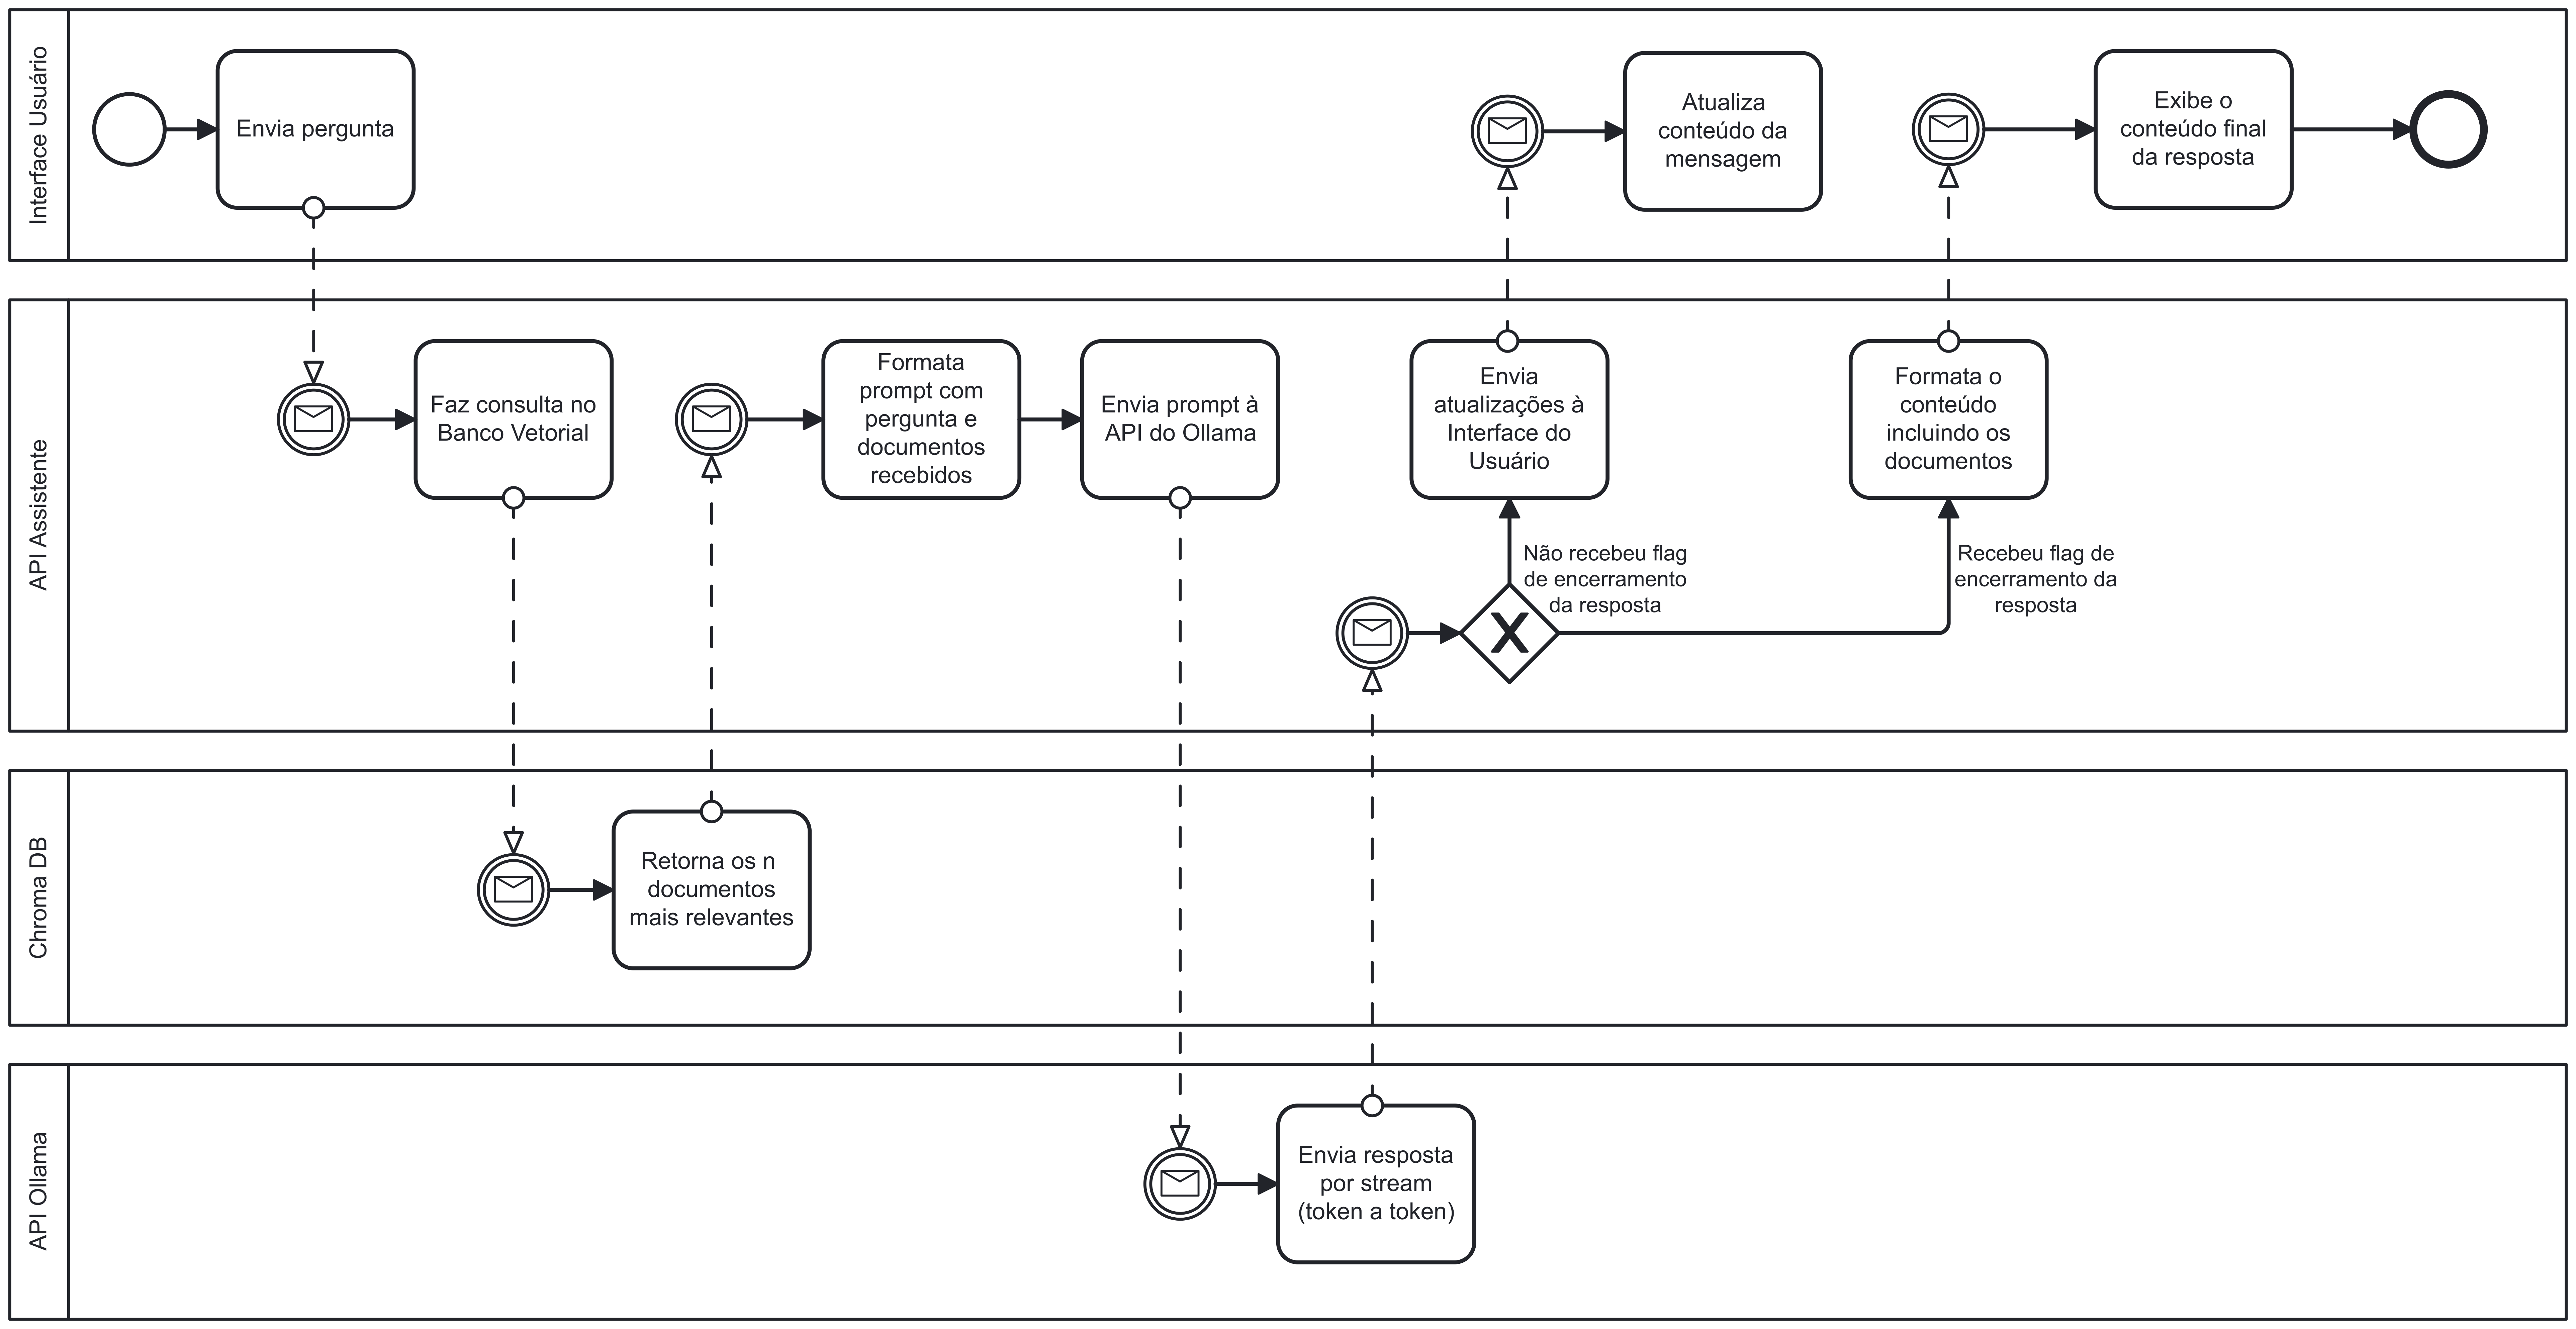
\includegraphics[width=1\linewidth]{Imagens/diagram.png}
    \caption{Diagrama de Atividades do Assistente de Busca}
    Fonte: autoria própria
    \label{fig:diag-atividade-assist-busca}
\end{figure}

Além de incluir a pergunta, a resposta e o conjunto de documentos que foram utilizados na composição do \textit{prompt} enviado ao \ac{LLM}, a API Gerenciadora de Fluxo coleta dados a respeito do processo como um todo (tempo levado na execução de cada etapa, métricas utilizadas, dentre outros) e os inclui na resposta devolvida ao usuário. Também cabe a esse elemento garantir persistência de dados sobre cada uma das interações realizadas, permitindo que, a posteriori, sejam analisados e utilizados para refinamento do processo e da estrutura proposta. Por conveniência e compatibilidade com as estruturas de armazenamento já existentes na Alern, os dados das interações serão salvos em bancos Relacionais.

\section{Interface de Usuário}
\label{sec:Metodologia.5}

Dado o objetivo deste estudo, foi definida uma página \textit{web} como interface de usuário -- considerando sua simplicidade de desenvolvimento e implementação -- nos moldes de uma aplicação de envio/recebimento de mensagens de texto, como é o mais comum ao se desenhar uma ferramenta de \textit{chatbot}, conforme visto na Figura \ref{fig:interface-assist-busca}.

\begin{figure}[H]
    \centering
    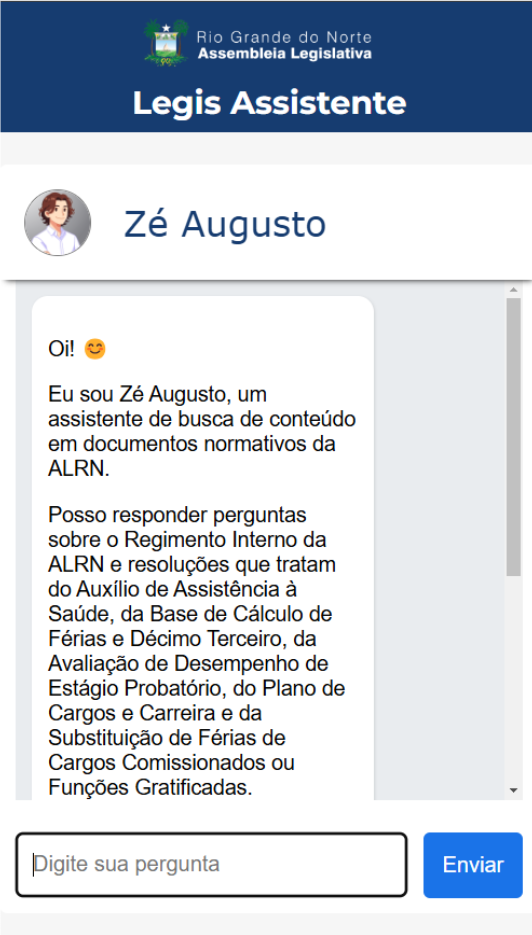
\includegraphics[width=0.5\linewidth]{Imagens/interface_usuario.png}
    \caption{Interface de Usuário Inicial do Assistente de Busca}
    Fonte: autoria própria
    \label{fig:interface-assist-busca}
\end{figure}

A opção foi feita por manter uma interface limpa e minimalista, restringindo-se somente ao campo de envio de mensagens do usuário, bem como uma área superior com a exibição das mensagens enviadas e recebidas. Para isso, utilizamos uma página HTML simples, sem utilização de qualquer \textit{framework} ou tecnologia mais elaborada, valendo-se de Javascript para estabelecer comunicação com a API, receber os resultados e alterar elementos na interface em si, à medida que o usuário interage com a ferramenta.

Quando cada resposta é recebida, o usuário pode escolher avaliar a resposta recebida como satisfatória, como uma resposta ruim, ou ainda reportar a resposta como contendo conteúdo indevido -- mostrado na Figura \ref{fig:interface-assist-busca-resposta}. As avaliações dos usuários serão utilizadas para análise e como recursos para, eventualmente, criar um conjunto de dados que permita futuro refinamento dos modelos utilizados.

\begin{figure}[H]
    \centering
    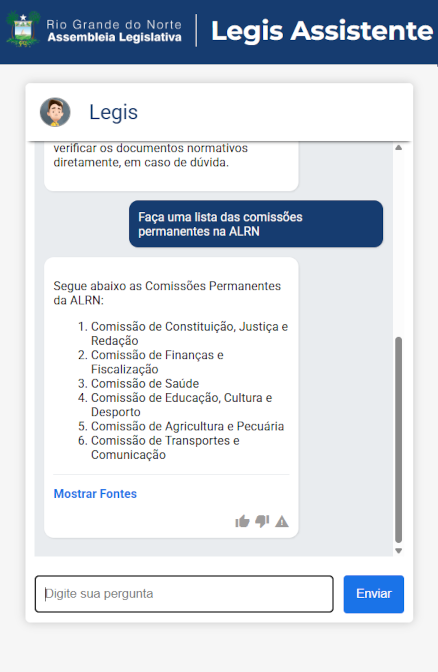
\includegraphics[width=0.5\linewidth]{Imagens/interface_usuario_resposta.png}
    \caption{Interface de Usuário do Assistente de Busca com Resposta}
    Fonte: autoria própria
    \label{fig:interface-assist-busca-resposta}
\end{figure}

Optamos, para fins de simplicidade, manter uma abordagem em que as perguntas e respostas do usuário são voláteis, de forma que, para o usuário, não há continuidade entre as sessões de uso. Cada sessão (marcada pelo carregamento da página de \textit{chat}) se inicia com um histórico limpo de interações, de forma que a persistência dos dados das interações é feita e mantida somente para fins de avaliação, sem ser retomada pelo usuário em qualquer momento futuro.

A mecânica de consulta consiste apenas de uma solicitação realizada à API de gerenciamento do fluxo de informações, por meio de requisição HTTP, que envia a pergunta ou frase de consulta a ser utilizada como critérios de busca no banco vetorial, bem como um vetor de \textit{embeddings} contendo os dados das interações mais recentes, o qual será utilizado como informação do contexto, junto ao \ac{LLM}, de forma a manter um senso de continuidade no \textit{chat}.

\section{Medição dos Resultados}
\label{sec:Metodologia.6}
Considerando a natureza da tarefa a que se propõe a aplicação objeto deste estudo (especificamente o resultado final do processo), entende-se que uma avaliação criteriosa feita por um humano seria o adequado para aferir se a resposta dada é satisfatória para a pergunta ou consulta realizada. Em um cenário ideal, esse avaliador também teria conhecimento aprofundado do domínio no qual a aplicação atua, de forma a garantir que não somente a resposta é coerente, mas também se o conhecimento que ela se pretende a suprir está acurado. Esse tipo de avaliação, contudo, por sua própria natureza, demanda tempo -- que acaba por ser ainda mais custoso, por envolver um especialista numa área de domínio -- e se mostra pouco escalável, dado que o volume de amostras a serem avaliadas fica restrito à disponibilidade de avaliadores.

Ainda assim, uma das formas de avaliação do desempenho do Assistente de Busca como um todo a que pretendemos é do tipo qualitativa, baseando-se no parecer dado por especialistas nas matérias de que trata o corpus documental que foi selecionado para o desenvolvimento e testes. O grupo de especialistas inclui, dentre outros, servidores atuantes na \ac{CDHO}, da Assembleia Legislativa do Rio Grande do Norte, dado que a prática diária de suas atividades os torna familiarizados com os meandros das Resoluções e definições regimentais contidas na seleção de documentos abordada neste estudo.

Assim, interagiriam os especialistas com a interface de usuário, inserindo perguntas sobre aspectos relevantes cobertos pelos atos normativos no conjunto de documentos selecionados. As interações dos especialistas não serão guiadas ou direcionadas, de forma que as perguntas feitas sejam orgânicas e o mais próximo possível do tipo de uso que o Assistente de Busca terá após sua implementação e disponibilização. Os avaliadores observarão as respostas geradas, aferindo quantitativamente a sua exatidão e fornecendo eles mesmos um texto breve com o teor do que deveria ser a resposta ideal.

Os dados coletados da interação serão armazenados para análise posterior, e, a depender da quantidade de dados coletados, utilizados para eventual refinamento e ajuste fino dos modelos que servem de base para as camadas da ferramenta.

Não obstante, há um aspecto relevante a ser considerado, o qual potencialmente emergirá das condições de avaliação propostas. Dado que os especialistas farão perguntas sem direcionamento, é improvável que o conjunto total de perguntas submetidas ao Assistente de Busca tenha uma variedade grande o suficiente para abordar toda a amplitude de matérias presentes nos documentos. Perguntas repetidas, aspectos sobre os quais não lhes ocorrerá perguntar, assuntos cuja natureza seja considerada demasiadamente óbvia para questionamento, entre outros, são alguns dos problemas cuja ocorrência pode ser prevista com algum grau de confiança.

No que concerne à avaliação realizada pelos especialistas, além da possível falta de cobertura das perguntas feitas, há outro ponto delicado cuja abordagem é relevante. Dado que a avaliação dos especialistas em relação ao Assistente, da forma como descrita, se debruça somente sobre o resultado final do processo -- a resposta -- a identificação de possíveis elementos responsáveis pela qualidade aquém da esperada se torna menos efetiva, posto que são perdidas informações dos processos intermediários da geração da resposta. Nessas condições, embora seja possível a identificação de respostas inadequadas, os dados não são suficientes para determinar se a falha ocorreu na recuperação dos documentos junto ao banco vetorial ou se a resposta gerada pelo \textit{Llama} foi incorreta, mesmo com as informações adequadas disponíveis.

Com o fim de mitigar esses dois problemas apontados, serão feitas avaliações utilizando uma abordagem diferente, buscando garantir cobertura tanto da totalidade do conteúdo no banco vetorial quanto a verificação de resultados intermediários que são elementos base para a geração da resposta final. Analisaremos o seguinte:

\begin{itemize}
    \item o quanto os resultados das buscas no banco vetorial são pertinentes às perguntas, comparando os modelos (avaliação automatizada quantitativa);
    \item o tempo de execução/latência nas buscas no banco vetorial (avaliação automatizada quantitativa);
    \item a qualidade da resposta final gerada pelo Assistente (avaliações humana qualitativa e automatizada quantitativa).
\end{itemize}

De forma a alcançar esse objetivo, com base no conteúdo existente no banco vetorial, geraremos sinteticamente um conjunto de dados que permitirá explorar cada uma das etapas do processo de geração de respostas, possibilitando avaliar os resultados intermediários e finais da aplicação. Especificamente, esse conjunto terá, para cada um dos fragmentos inclusos no banco vetorial, o seguinte:

\begin{enumerate}
    \item uma lista de perguntas baseadas no conteúdo do fragmento;
    \item uma lista de respostas de referência para cada uma dessas perguntas, compostas por trechos do respectivo fragmento;
    \item um conjunto com os 10 fragmentos com maior similaridade semântica com a pergunta, obtidos do banco vetorial;
    \item uma resposta final para a pergunta, gerada pelo Assistente.
\end{enumerate}

A abordagem, portanto, para avaliar o grau de eficácia dos modelos de \textit{embeddings} consiste em, dado que sabemos qual o fragmento original que foi utilizado para geração de cada uma das perguntas, analisar seu respectivo conjunto de fragmentos de documentos recuperados do banco vetorial e observar se o fragmento original é um de seus elementos. No que concerne à validação da resposta final gerada, pode ser utilizada a métrica \textit{BERTScore} de similaridade entre a resposta final e a resposta de referência.

Como meio de automação da tarefa de geração do conteúdo base, tomamos a decisão de utilizar um segundo \ac{LLM} parametrizado com o objetivo específico de gerar tanto o conjunto de perguntas quanto o de respostas. Com a ciência de que, na prática, teremos um conteúdo gerado por um \ac{LLM} (a resposta final) sendo avaliado com base em um conteúdo também gerado por um \ac{LLM} (a resposta de referência), definimos, como forma de prover um mínimo de independência, que utilizaríamos modelos diferentes para a execução de cada uma das tarefas. Uma vez que optamos pelo \textit{Llama3.1} como \ac{LLM} a integrar a arquitetura do Assistente de Busca, adotamos o \textit{GPT-4o} \cite{GPT4o:1} para a geração das perguntas e respostas -- tanto por ser não relacionado com os modelos sendo avaliados (\textit{Llama3.1} e \textit{DeepSeek-r1}), como também pela reconhecida qualidade de conteúdo gerado.


\subsection{Processo de Geração dos Dados de Teste}
\label{subsec:Metodologia.6.1}


Para a efetiva geração dos dados a serem utilizados com testes e avaliações, cada um dos fragmentos documentais foi utilizado em um \textit{prompt} de geração de conteúdo a ser processado por uma instância do modelo \textit{GPT-4o}, da OpenAI (por meio da API fornecida pela OpenAI, para consulta externa). O teor do \textit{prompt} é como segue:

\begin{quote}
{
    \footnotesize
    \ttfamily
    \raggedright
    \sloppy
    Considere o texto a seguir, que é um artigo de uma lei:
    
    \{artigo\}
    
    Agora extraia as informações do artigo e gere perguntas que possam ser respondidas com base no conteúdo textual do artigo.
    
    Além disso, formule a resposta com base no artigo e em nenhuma outra fonte. As perguntas e respostas serão utilizadas para treinamento e \textit{finetuning} de um LLM. Siga as seguintes diretrizes para gerar as perguntas e respostas:

    Considere o texto recebido e identifique informações significativas;
    
    Com base nas informações, crie pelo menos 3 perguntas que possam ser respondidas com base no conteúdo do texto;
    
    Caso o texto fornecido não tenha informação a partir da qual seja possível criar perguntas relevantes, deve ser retornado um objeto vazio;
    
    As perguntas devem ser claras, diretas, e específicas;
    
    As perguntas podem ter sinônimos ou termos aproximados do texto base, mas devem ser possível de ser respondidas pelo texto fornecido;
    
    Para cada pergunta, formule uma resposta usando como base o conteúdo do artigo, sem utilizar qualquer outro conhecimento que você disponha.

    Cada pergunta será aceitável somente se:

    * Estiver relacionada aos assuntos pertinentes ao artigo apresentado
    
    * For uma pergunta relevante, semelhante ao que seria perguntado por uma pessoa com dúvida
    
    * Puder ser respondida usando o fragmento apresentado

    O resultado deve ser em formato estruturado, em formato JSON, sendo uma lista de objetos assim:
    
    [\{``pergunta'': ``texto da pergunta'', ``resposta'':``texto da resposta''\},
    
     \{``pergunta'': ``texto da pergunta'', ``resposta'':``texto da resposta''\}]
    
    Não deve haver nenhum outro texto, apenas a lista.

    Um exemplo de como devem ser geradas as perguntas:

    Exemplo de texto base:
    
    ``Art. 1º A Assembleia Legislativa é composta de Deputados, representantes do povo norte-rio-grandense, eleitos, na forma da lei, para mandato de 4 (quatro) anos.''

    Resultado aceitável:
    
        [\{``pergunta'': ``A Assembleia Legislativa é formada pelo que?'', ``resposta'': ``A Assembleia Legislativa é composta por Deputados, que são eleitos pelo do povo norte-rio-grandense e os representam.'',\},
            
        \{``pergunta": ``O que é um Deputado?",``resposta": ``Um Deputado é um representante eleito do povo, possuindo mandato de quatro anos.''\},
        \{``pergunta'': ``Quanto tempo dura um mandato?'',``resposta'': ``Um mandato dura pelo período de quatro anos.''\}]

    Caso o texto não tenha conteúdo relevante, o resultado deve ser um objeto vazio \{\}.

    Vamos começar?
}
\end{quote}

O resultado gerado pelo \textit{GPT-4o} foi analisado com fins de assegurar sua correção em termos de formato JSON, para garantir que o arquivo estivesse válido e pudesse ser usado no processo de avaliação. Dessa forma, cada fragmento no banco vetorial recebeu um conjunto de perguntas, acompanhado de suas respectivas respostas, geradas com base no texto do próprio fragmento, sendo, portanto, ambas diretamente relacionadas ao conteúdo que lhes deu origem. Essas respostas para as perguntas elaboradas serão utilizadas como resposta de referência ao se avaliar a qualidade do conteúdo das respostas finais geradas pelo \ac{LLM} integrante do Assistente de Busca, por meio do \textit{BERTScore}, conforme descrito na Seção \ref{subsec:Resultados.2.2}. A Figura \ref{fig:geracao-perguntas} resume o processo de geração das perguntas e respostas.

\begin{figure}[H]
    \centering
    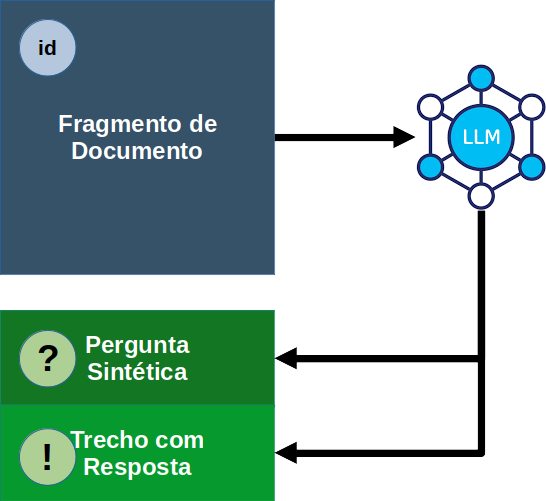
\includegraphics[width=0.5\linewidth]{Imagens/geracao-perguntas.png}
    \caption{Geração de pares pergunta-resposta por meio de LLM}
    Fonte: autoria própria
    \label{fig:geracao-perguntas}
\end{figure}

Após a geração do conjunto de perguntas ``sintéticas'' para cada fragmento, cada pergunta foi usada para realizar buscas no banco vetorial com o objetivo de identificar documentos semanticamente semelhantes. Como resultado, para cada pergunta associada a um fragmento, foi gerado um conjunto de documentos considerados semanticamente próximos (ver Figura \ref{fig:recuperacao-fragmentos}).

\begin{figure}[H]
    \centering
    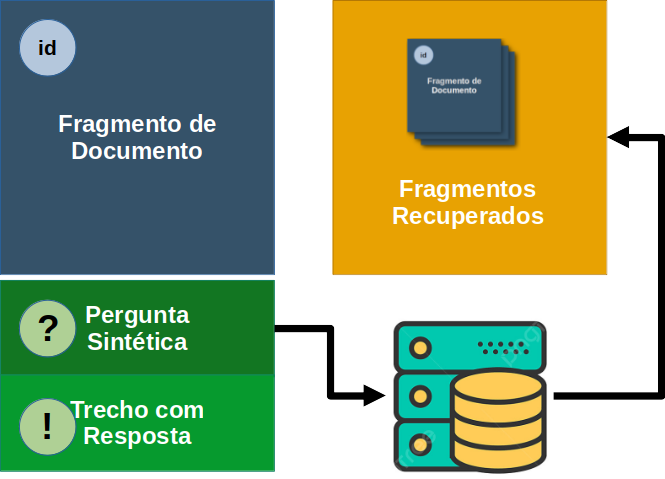
\includegraphics[width=0.5\linewidth]{Imagens/recuperacao-fragmentos.png}
    \caption{Recuperação de documentos do Banco Vetorial}
    Fonte: autoria própria
    \label{fig:recuperacao-fragmentos}
\end{figure}

Com as perguntas e seus correspondentes conjuntos de documentos relevantes, foi possível utilizar esses materiais, conforme detalhado na Seção \ref{sec:Metodologia.3}, para criar um \textit{prompt} e solicitar ao \textit{Llama} que gerasse uma resposta completa baseada na seleção de documentos. Esse processo emula a dinâmica seguida pelo Assistente de Busca durante seu uso comum pelos usuários, simulando uma interação que visa fornecer respostas completas e relevantes a partir de consultas realizadas (Figura \ref{fig:geracao-respostas}).

\begin{figure}[H]
    \centering
    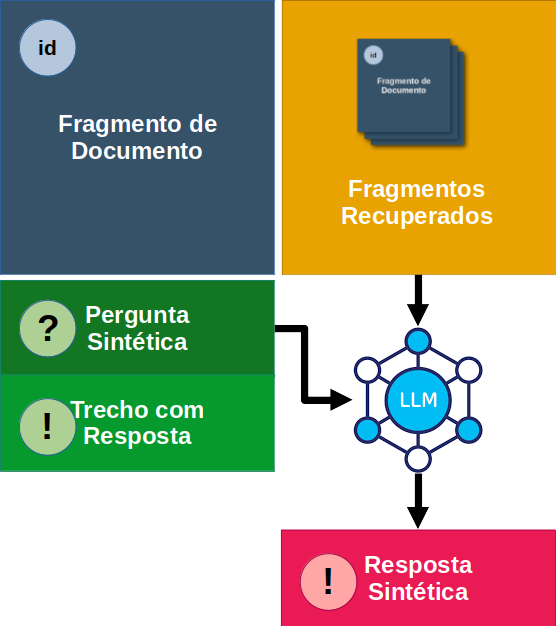
\includegraphics[width=0.5\linewidth]{Imagens/geracao-respostas.png}
    \caption{Recuperação de documentos do Banco Vetorial}
    Fonte: autoria própria
    \label{fig:geracao-respostas}
\end{figure}

Havendo sido concluídas todas essas etapas, foi possível obter, para cada pergunta gerada sinteticamente, uma estrutura de dados como a apresentada na Tabela \ref{tab:dados-sinteticos}. Esses dados gerados possibilitam não somente a abordagem de mitigação dos problemas apontados, como também a realização de uma avaliação preliminar também automatizada, com foco nas duas etapas de geração das respostas: a recuperação de documentos por similaridade, junto ao banco vetorial, e a elaboração do texto final da resposta feita pelo \textit{Llama}, com base no teor dos documentos selecionados.

\begin{table}[H]
    \caption{Estrutura dos dados sintéticos gerados para cada fragmento}
    \centering
    \begin{tabular}{ l p{10cm} }
         \hline
         \textbf{Informação} & \textbf{Descrição} \\  
         \hline
         Id & Identificador do fragmento usado para gerar a pergunta \\
         Pergunta & Pergunta gerada pelo \textit{GPT-4} com base no fragmento \\
         Resposta & Proposta de resposta do \textit{GPT-4} para a pergunta gerada \\
         Fragmentos & Lista de fragmentos relevantes recuperados do banco de vetores \\
         Resposta \textit{Llama} & Resposta gerada pelo \textit{Llama} com base na pergunta e nos fragmentos relevantes \\
         \hline
    \end{tabular}
    
    Fonte: O autor (2024)
    \label{tab:dados-sinteticos}
\end{table}

\subsection{Avaliação da Recuperação de Conteúdo (\textit{Retrieval})}
\label{subsec:Metodologia.6.2}
Como forma de avaliar a recuperação dos fragmentos realizada pelo banco de vetores, é possível lançar mão de dois campos presentes na estrutura de dados apresentada na Tabela \ref{tab:dados-sinteticos}, a saber: Id (que contém o identificador do fragmento utilizado para gerar a pergunta) e Fragmentos (que contém os fragmentos recuperados do banco vetorial). Consideremos que cada pergunta foi gerada com base no conteúdo de um fragmento específico de documento. A partir disso, é possível assumir que é natural que exista uma similaridade entre o teor da pergunta e o do fragmento original. Pelos mesmos motivos, também é esperado que, entre os fragmento recuperados na avaliação de semelhança semântica, esteja incluído o próprio fragmento que serviu de base para a criação da pergunta.

Adicionalmente, considerando que é possível recuperar o conteúdo do fragmento base -- gerador da pergunta -- bem como obter o texto dos fragmentos retornados pelo banco vetorial, existe uma abordagem alternativa à verificação do grau de similaridade entre a pergunta e os fragmentos retornados. Em vez de se lançar mão da pergunta, utiliza-se como parâmetro de avaliação a similaridade entre o conteúdo do fragmento base com os textos dos fragmentos retornados.

Em suma, para cada pergunta sintética utilizada, avaliaremos se o id do fragmento original, utilizado para gerar a pergunta, figura entre os ids do conjunto de fragmentos retornados do banco vetorial. Consideraremos bem sucedida a execução do processo caso haja a presença do id alvo no conjunto de fragmentos recuperados.

Dentro do conjunto textual, os documentos articulados correspondem a textos normativos sobre temas específicos, de forma que há muito pouco de sobreposição de temas entre eles. O documento não articulado (Manual de Processo Legislativo -- listado como documento 12 nas Tabelas \ref{tab:descricao-documentos-1} e \ref{tab:descricao-documentos-1}), contudo, aborda muito do que é tratado na Resolução Nº 031/2021 (O Regimento Interno da Alern, presente nas Tabelas \ref{tab:descricao-documentos-1} e \ref{tab:descricao-documentos-1} como documento 2), detalhando os meandros do processo legislativo. Portanto, é natural que haja uma grande interseção de assuntos neles presentes.

Como forma de averiguar o desempenho dos modelos diante de variados cenários de documentos, realizaremos os testes com três configurações distintas, em termos de diversidade das temáticas abordadas pelos documentos, bem como de suas estruturas. 

\begin{itemize}
    \item Recuperação dos fragmentos \textit{somente dos documentos articulados}, cada um deles referente a um assunto exclusivo, não majoritariamente abordado por outros documentos;
    \item Recuperação dos fragmentos de documentos articulados e do documento estruturado (Manual de Processo Legislativo) -- o que inclui uma quantidade considerável de sobreposição de conteúdo entre os elementos; e
    \item Recuperação de fragmentos de um conjunto de dados textuais sem qualquer restrição de sobreposição temática, utilizando o conteúdo publicado na página de notícias da Alern, mantida pela Coordenadoria de Comunicação da Casa, para fins de comparação de performance.
\end{itemize} 


O conjunto de textos da terceira abordagem é composto por mais de mil notícias relacionadas especificamente a sessões ordinárias e reuniões de comissões, as quais tratam de sumarizar os pontos mais relevantes das discussões travadas e das propostas apresentadas pelos parlamentares. São textos lineares e não possuem qualquer tipo de estrutura ou hierarquia definida -- salvo pela existência de um título, que dá um indicativo do seu conteúdo. Então como estratégia de particionamento, nos limitamos a dividir as notícias por parágrafo, para ser o conjunto de fragmentos e prepusemos o texto do título da notícia, como forma de lhes garantir um mínimo de contexto. A Tabela \ref{tab:descricao-noticias} descreve os aspectos da do conjunto de dados.

\begin{table}[H]
    \caption{Descrição do dataset de notícias}
    \centering
    \begin{tabular}{ l r }
        \hline
        \bfseries Característica & \bfseries Valor \\
        \hline
        Media de Fragmentos por notícia & 5,6 \\
        Media de Tamanho & 299,8 \\
        Quantidade de Notícias & 1.436 \\
        Quantidade de Fragmentos & 8.044 \\
        \hline
    \end{tabular}
    
    Fonte: O autor (2025)
    \label{tab:descricao-noticias}
\end{table}

\subsection{Avaliação das Respostas Geradas pelo LLM}
\label{subsec:Metodologia.6.3}
A avaliação da qualidade das respostas geradas pelo \ac{LLM} é um aspecto fundamental para garantir a eficácia e a confiabilidade das respostas geradas com base nos documentos recuperados. Uma avaliação eficaz não deve se limitar a quantificar a similaridade entre a resposta gerada e a pergunta original. Em vez disso, foca na capacidade de a resposta satisfazer as expectativas informacionais do usuário. Essa abordagem assegura que as respostas não apenas sejam relevantes em um sentido superficial, mas que realmente atendam aos critérios de completude e precisão em relação ao corpus documental utilizado.

Embora a similaridade entre a pergunta e a resposta seja uma métrica viável, demonstra-se insuficiente para avaliar a qualidade da resposta em um nível mais profundo. A análise de proximidade semântica da resposta em relação à pergunta não garante que a resposta abranja de forma adequada o contexto e o conteúdo desejado pelo próprio fato de que uma resposta, por definição, deve conter informações inexistentes na pergunta. Portanto, a avaliação deve ir além da correspondência superficial e considerar o quão bem a resposta aborda e resolve a questão apresentada.

\subsubsection{Avaliação Automatizada}
\label{subsubsec:Metodologia.6.3.1}
Para avaliar a qualidade das respostas em termos de satisfação da pergunta, ferramentas como o BERTScore, proposto por \citeonline{BERTScore:1}, abordado na Seção \ref{sec:Teorico.7}, se mostram úteis. Sua aplicação em sistemas de \ac{RAG} oferece uma maneira objetiva de quantificar o desempenho dos \ac{LLM}s no que tange à satisfatoriedade de suas respostas às perguntas. Essa métrica considera a semelhança semântica e permite identificar se uma resposta contém informações relevantes e está alinhada com o que foi solicitado pela pergunta. Assim, como métrica de avaliação da resposta final gerada utilizamos o BERTScore sobre a resposta, gerada para cada uma das perguntas sintéticas disponíveis, em relação à sua respectiva resposta de referência (ver Seção \ref{subsec:Metodologia.6.1}), dado que este contribui para a validação da qualidade da resposta gerada, não apenas em termos de similaridade de palavras, mas em relação à precisão e completude, características essenciais para a construção de sistemas de perguntas e respostas de alta qualidade. Como resultado, se alcança uma medida mais robusta de como a resposta aborda de maneira contextualizada a pergunta, indo além da análise de correspondência lexical.

Cabe pontuar, contudo, que o BERTScore servirá tão somente como uma ferramenta quantitativa de avaliação das respostas, motivo pelo qual utilizaremos avaliação humana para dar conta de aspectos mais qualitativos das respostas.

\subsubsection{Avaliação Humana}
\label{subsubsec:Metodologia.6.3.2}
A avaliação humana da qualidade das respostas geradas se debruçará sobre dois aspectos do produto final da aplicação \ac{RAG}: as características estruturais do texto gerado e o conteúdo gerado, em si.

Inicialmente, será conduzida uma investigação exploratória sobre o material produzido pelos modelos, com o objetivo de obter uma visão panorâmica e destacar eventuais irregularidades evidentes, perceptíveis sem necessidade de exame detalhado. Entre esses aspectos, serão observados o comprimento das respostas, a lógica de suas construções textuais, a uniformidade no uso do idioma, bem como outras possíveis anomalias que possam surgir no decorrer da análise.

Após isso, uma análise mais estruturada e sistemática será feita das respostas, baseando-se em perguntas orgânicas -- feitas por avaliadores humanos, em vez de perguntas sintéticas. Para isso, contaremos com a ajuda de servidores da \ac{Alern}, aos quais será solicitado que elaborem perguntas que possam ser respondidas através de conteúdo presente nos documentos integrantes do nosso conjunto de dados, juntamente com suas respectivas respostas. As perguntas serão utilizadas para gerar respostas, seguindo todo o fluxo da aplicação \ac{RAG} (recuperação de documentos, formatação do conteúdo, injeção do resultado para criação de um \textit{prompt} e sua submissão à API da ferramenta de execução de \ac{LLM}s, para geração da resposta). Ao todo, 4 servidores colaborarão para esta parte do processo, gerando um total de 20 perguntas.

Após isso, as respostas serão apresentadas aos avaliadores, os quais receberão direcionamento para avaliar as respostas sob os seguintes critérios:

\begin{itemize}
    \item Corretude: avalia o quão correta a resposta está, tanto em termos de não apresentar informações falsas, quanto em termos de responder a pergunta;
    \item Coerência: avalia o quanto o teor da resposta (correta ou não) está escrito de forma coerente -- apresenta sentido coerente, incluindo mostrar consistência no idioma utilizado;
    \item Gramática e Ortografia: avalia se as palavras utilizadas estão corretamente grafadas e se as frases têm escrita gramaticalmente correta;
    \item Adequação: avalia se o nível de escrita apresenta vocabulário adequado à compreensão do usuário comum, conforme definido nas diretrizes passadas via \textit{prompt}.
\end{itemize}

Para cada um dos critérios, o avaliador deverá atribuir um valor de 0 nos casos em que a pergunta gerada tiver um desempenho ``ruim'', 1 para um desempenho ``aceitável'' ou 2 para um desempenho ``bom'' / plenamente satisfatório. Para cada um dos modelos utilizados, será calculado o somatório dos pontos em cada um dos critérios e a porcentagem da pontuação máxima possível de ser alcançada.

Os resultados das avaliações humanas serão, após o processo, compilados e quantificados, de forma a permitir uma melhor compreensão da qualidade dos resultados gerados pela ferramenta.


\subsection{Nota Sobre a Estrutura Utilizada para os Experimentos}
\label{subsec:Metodologia.6.4}

Os experimentos de testes descritos neste estudo foram implementados por meio de \textit{scripts} desenvolvidos na linguagem de programação Python e armazenados em um \href{https://github.com/saintclairlima/assistente-busca}{repositório público no GitHub} \cite{REPOSITORIO:1}, tanto para fins de transparência, quanto para fins de agilizar e simplificar o processo de execução, independente do local e da máquina utilizada. Devido à indisponibilidade de \textit{hardware} local adequado para a execução dos testes -- especialmente considerando a alta demanda computacional associada à utilização de modelos de \ac{LLM}s em execução paralela com uma instância do Ollama com o \textit{Llama3.1:8b} e o \textit{DeepSeek-r1:7b} -- optou-se por clonar o repositório em instâncias do Google Colab para a condução dos experimentos. Essa abordagem garantiu acesso a recursos computacionais menos limitados, mitigando as restrições do ambiente local.

O ambiente de execução no Google Colab foi configurado com uma GPU NVIDIA Tesla T4, que dispõe de 16 GB de memória dedicada, sendo a configuração padrão de utilização gratuita da plataforma \cite{HARDWARE:1, HARDWARE:2}. Essa arquitetura foi fundamental para permitir a execução eficiente de modelos pesados, assegurando um desempenho adequado tanto para o processo de recuperação de documentos do banco vetorial, quanto para a execução do modelo \textit{Llama} para gerar as respostas. A integração entre os recursos oferecidos pelo Google Colab e as capacidades do Ollama foi configurada de forma a maximizar a compatibilidade e o desempenho dos experimentos.

Por meio dessa infraestrutura, foi possível realizar os testes necessários sem comprometer a validade dos resultados, assegurando que a execução dos experimentos fosse realizada de maneira confiável e reprodutível. Adicionalmente, a utilização do repositório GitHub \cite{REPOSITORIO:1} como plataforma para versionamento e controle do código contribuiu para a transparência e rastreabilidade das implementações, elementos essenciais em um contexto de pesquisa científica.

% ----------------------------------------------------------
% Finaliza a parte (textual) no bookmark do PDF
% para que se inicie o bookmark na raiz
% e adiciona espaço de parte no Sumário
% ----------------------------------------------------------
\phantompart

% ----------------------------------------------------------
% ELEMENTOS PÓS-TEXTUAIS
% ----------------------------------------------------------
\postextual

% ----------------------------------------------------------
% Referências bibliográficas
% ----------------------------------------------------------
\bibliography{referencias}

% ----------------------------------------------------------
% Apêndices
% ----------------------------------------------------------
% ---
% Inicia os apêndices
% ---
\begin{apendicesenv}

% Imprime uma página indicando o início dos apêndices
\partapendices
% ----------------------------------------------------------
\chapter{Conteúdos da Avaliação do Texto das Respostas}
\label{apendice:apendice1}
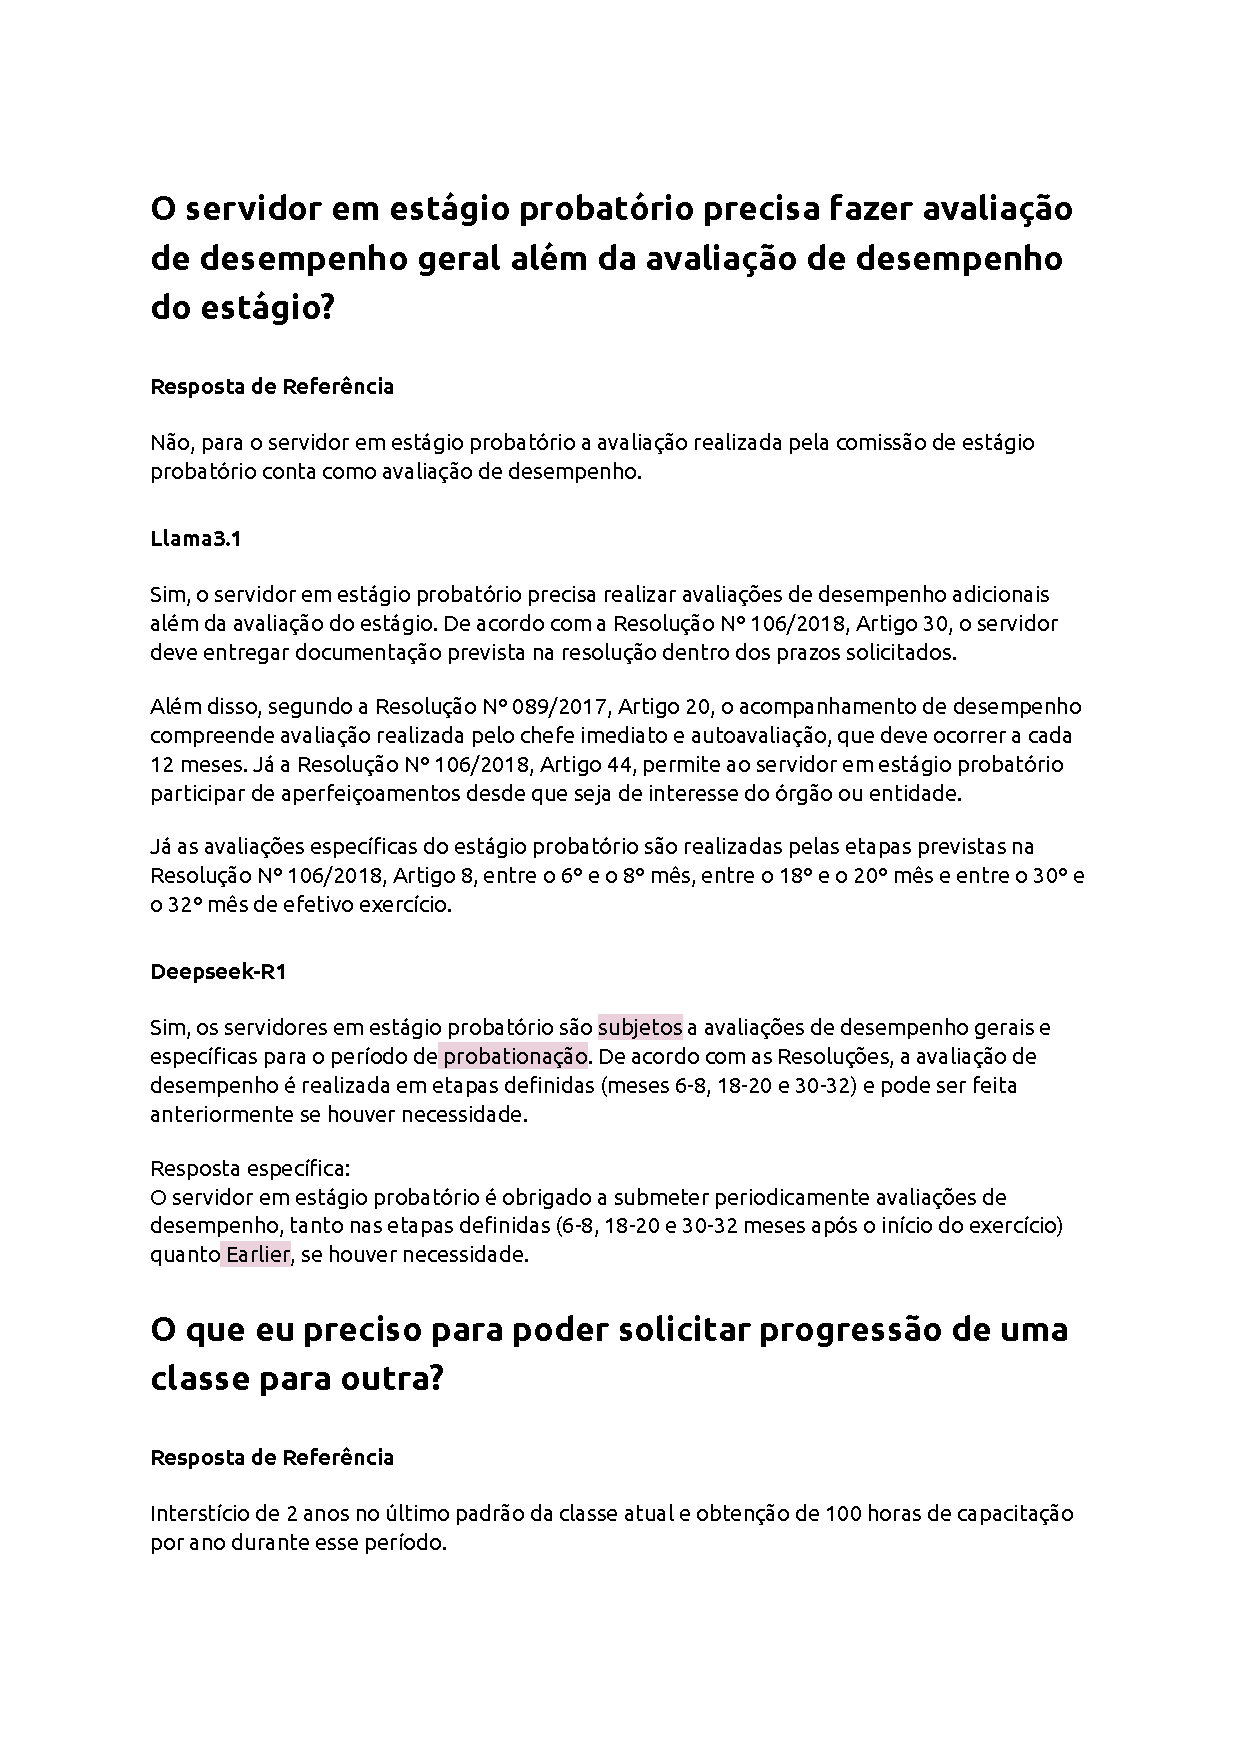
\includepdf[pages=-]{Anexos/comparativo-respostas.pdf}
\end{apendicesenv}

% ----------------------------------------------------------
% Anexos
% ----------------------------------------------------------
\input{Includes/Anexos.tex}

%---------------------------------------------------------------------
% INDICE REMISSIVO
%---------------------------------------------------------------------

\phantompart
\printindex
%---------------------------------------------------------------------

\end{document}
